%----------------------------------------------------------------------------------------
%	PACKAGES AND OTHER DOCUMENT CONFIGURATIONS
%----------------------------------------------------------------------------------------

\documentclass[
11pt, % The default document font size, options: 10pt, 11pt, 12pt
%oneside, % Two side (alternating margins) for binding by default, uncomment to switch to one side
english, % ngerman for German
singlespacing, % Single line spacing, alternatives: onehalfspacing or doublespacing
%draft, % Uncomment to enable draft mode (no pictures, no links, overfull hboxes indicated)
%nolistspacing, % If the document is onehalfspacing or doublespacing, uncomment this to set spacing in lists to single
%liststotoc, % Uncomment to add the list of figures/tables/etc to the table of contents
%toctotoc, % Uncomment to add the main table of contents to the table of contents
%parskip, % Uncomment to add space between paragraphs
%nohyperref, % Uncomment to not load the hyperref package
headsepline, % Uncomment to get a line under the header
%chapterinoneline, % Uncomment to place the chapter title next to the number on one line
%consistentlayout, % Uncomment to change the layout of the declaration, abstract and acknowledgements pages to match the default layout
]{MastersDoctoralThesis_updated} % The class file specifying the document structure

\usepackage[utf8]{inputenc} % Required for inputting international characters
\usepackage[T1]{fontenc} % Output font encoding for international characters

\usepackage{palatino} % Use the Palatino font by default

\usepackage[backend=biber,style=authoryear,natbib=true,maxbibnames=10]{biblatex} % Use the bibtex backend with the authoryear citation style (which resembles APA)

\addbibresource{zotero_sorted.bib} % The filename of the bibliography

\usepackage[autostyle=true]{csquotes} % Required to generate language-dependent quotes in the bibliography

\usepackage{gensymb}

% https://tex.stackexchange.com/questions/142148/typeset-one-citation-with-all-authors
\makeatletter
\newcommand{\tempmaxup}[1]{\def\blx@maxcitenames{\blx@maxbibnames}#1}
\makeatother

\DeclareCiteCommand{\longfullcite}[\tempmaxup]
  {\usebibmacro{prenote}}
  {\usedriver
     {\DeclareNameAlias{sortname}{default}}
     {\thefield{entrytype}}}
  {\multicitedelim}
  {\usebibmacro{postnote}}

%\DeclareDelimFormat[cbx@textcite]{nameyeardelim}{\addspace}

\usepackage{siunitx}

%----------------------------------------------------------------------------------------
%	MARGIN SETTINGS
%----------------------------------------------------------------------------------------

\geometry{
	paper=a4paper, % Change to letterpaper for US letter
	inner=2.5cm, % Inner margin
	outer=3.8cm, % Outer margin
	bindingoffset=.5cm, % Binding offset
	top=1.5cm, % Top margin
	bottom=1.5cm, % Bottom margin
	%showframe, % Uncomment to show how the type block is set on the page
}

%----------------------------------------------------------------------------------------
%	THESIS INFORMATION
%----------------------------------------------------------------------------------------

\thesistitle{Brain functional connectivity and~its~aberrations in mouse models of~autism} % \ttitle
\supervisor{Alessandro \textsc{Gozzi}} % \supname
\examiner{} % Your examiner's name, this is not currently used anywhere in the template, print it elsewhere with \examname
\degreen{Doctor of Philosophy} % \degreename
\author{Adam \textsc{Liska}} % \authorname
\addresses{} % Your address, this is not currently used anywhere in the template, print it elsewhere with \addressname

\subject{Biological Sciences} % Your subject area, this is not currently used anywhere in the template, print it elsewhere with \subjectname
\keywords{} % Keywords for your thesis, this is not currently used anywhere in the template, print it elsewhere with \keywordnames
\university{University of Trento} % \univname
\department{Doctoral School in Cognitive and Brain Sciences, University of Trento} % \deptname
\group{Center for Neuroscience and Cognitive Systems, Istituto Italiano di Tecnologia} % \groupname
\faculty{\href{http://faculty.university.com}{Faculty AAA Name}} % Your faculty's name and URL, this is used in the title page and abstract, print it elsewhere with \facname

\AtBeginDocument{
\hypersetup{pdftitle=\ttitle} % Set the PDF's title to your title
\hypersetup{pdfauthor=\authorname} % Set the PDF's author to your name
\hypersetup{pdfkeywords=\keywordnames} % Set the PDF's keywords to your keywords
}

\begin{document}

\frontmatter % Use roman page numbering style (i, ii, iii, iv...) for the pre-content pages

\pagestyle{plain} % Default to the plain heading style until the thesis style is called for the body content

%----------------------------------------------------------------------------------------
%	TITLE PAGE
%----------------------------------------------------------------------------------------

\begin{titlepage}
\begin{center}

\vspace*{.06\textheight}
{\scshape\LARGE \univname\par}\vspace{1.5cm} % University name
\textsc{\Large Doctoral Thesis}\\[0.5cm] % Thesis type

\HRule \\[0.4cm] % Horizontal line
{\huge \bfseries \ttitle\par}\vspace{0.4cm} % Thesis title
\HRule \\[1.5cm] % Horizontal line
 
\begin{minipage}[t]{0.4\textwidth}
\begin{flushleft} \large
\emph{Author:}\\
\authorname
\end{flushleft}
\end{minipage}
\begin{minipage}[t]{0.4\textwidth}
\begin{flushright} \large
\emph{Supervisor:} \\
\supname  
\end{flushright}
\end{minipage}\\[3cm]
 
\vfill

\large \textit{A thesis submitted in fulfillment of the requirements\\ for the degree of \degreename}\\[0.3cm] % University requirement text
\textit{in the}\\[0.4cm]
\deptname\\\groupname\\[2cm]
 
\vfill

{\large \today}\\[4cm] % Date
%\includegraphics{Logo} % University/department logo - uncomment to place it
 
\vfill
\end{center}
\end{titlepage}

%----------------------------------------------------------------------------------------
%	ABSTRACT PAGE
%----------------------------------------------------------------------------------------

\begin{abstract}
    \addchaptertocentry{\abstractname}
    Functional Magnetic Resonance Imaging (fMRI) has consistently highlighted
aberrant functional connectivity across brain regions of autism spectrum
disorder (ASD) patients. However, the manifestation and neural substrates of
these alterations are highly heterogeneous and often conflicting. Moreover,
their neurobiological underpinnings and etiopathological significance remain
largely unknown. A deeper understanding of the complex pathophysiological
cascade leading to impaired connectivity in ASD can greatly benefit from the use
of model organisms where individual pathophysiological or phenotypic components
of ASD can be recreated and investigated via approaches that are either off
limits or confounded by clinical heterogeneity.

In this work, we first describe the intrinsic organization of the mouse brain at
the macroscale as seen through resting-state fMRI (rsfMRI). The analysis of a
large rsfMRI dataset revealed the presence of six distinct functional modules
related to known brainwide functional partitions, including a homologue of the
human default-mode network (DMN). Consistent with human studies, interconnected
functional hubs were identified in several sub-regions of the DMN, in the
thalamus, and in small foci within integrative cortical structures such as the
insular and temporal association cortices.

We then study the effects of mutations in \textit{contactin associated
protein-like 2} (\textit{Cntnap2}), a neurexin-related cell-adhesion protein, on
functional connectivity.  Homozygous mutations in this gene are strongly linked
to autism and epilepsy in humans, and using rsfMRI, we showed that homozygous
mice lacking \textit{Cntnap2} exhibit aberrant functional connectivity in
prefrontal and midline functional hubs, an effect that was associated with
reduced social investigation, a core “autism trait” in mice.  Notably, viral
tracing revealed reduced frequency of prefrontal-projecting neural clusters in
the cingulate cortex of \textit{Cntnap2}$^{-/-}$ mutants, suggesting a possible
contribution of defective mesoscale axonal wiring to the observed functional
impairments.  Macroscale cortico-cortical white-matter organization appeared to
be otherwise preserved in these animals. These findings revealed a key
contribution of ASD-associated gene CNTNAP2 in modulating macroscale functional
connectivity, and suggest that homozygous loss-of-function mutations in this
gene may predispose to neurodevelopmental disorders and autism through a
selective dysregulation of connectivity in integrative prefrontal areas.

Finally, we discuss the role mouse models could play in generating and testing
mechanistic hypotheses about the elusive origin and significance of connectional
aberrations observed in autism and recent progress towards this goal.

\end{abstract}

%----------------------------------------------------------------------------------------
%	ACKNOWLEDGEMENTS
%----------------------------------------------------------------------------------------

\begin{acknowledgements}
    \addchaptertocentry{\acknowledgementname}
    The work presented in this thesis would not have been possible without the large
contribution of many people around me. First of all, I would like to thank my
advisor, Alessandro Gozzi, for all the guidance during the past few years.
Working with him has been formative from personal, professional and scientific
perspectives and it has also been a great experience. Moreover, the group of
people that Alessandro brought together in the Functional Neuroimaging Lab will
be difficult to beat elsewhere. Alberto Galbusera, Alessia de Felice, Carola
Canella, Daniel Gutierrez Barragan, Ludovico Coletta and Marco Pagani are great
colleagues and great friends and I really enjoyed working with them. A special
shout-out goes to Alberto for collecting most of the MRI data that I have worked
with. I would also like to thank all past members of the lab and other
collaborators: Alice Bertero, Anna Aksiuto, Gergely David, Manuel Blesa, Nayome
Rey Calvo and Richard Gomolka.

Pursuing a PhD, while stressful and often full of struggle, has also been a lot
of fun, both inside the office and outside. I immensely enjoyed all the trips,
hikes and aperitivi with my colleagues and other friends from CIMeC, IIT and
around: Germ\'{a}n Kruszewski, Georgiana Dinu, Jan B\'{i}m, Nghia The Pham and
many, many others with whom I have been lucky to share the beautiful city of
Rovereto and the mountains around.

Many thanks go to the administration of the Doctoral School and the Center for
Neuroscience and Cognitive Systems, namely to Leah Mercanti, Sara Maistrelli and
Paola Battistoni, for making all the paperwork a (mostly) smooth ride. I would
also like to thank the members of my oversight committee, Stefano Panzeri and
Jorge Jovicich, for all the feedback they provided.

My parents, Hana and Zbyn\v{e}k, and my brothers, Jan and Martin, provided a
great amount of support over the past years. Their visits in Rovereto were
always a source of joy!

Finally and above all, I would like to thank Angeliki, whose encouragements,
laughs and support made the start of our journey extraordinary.

\end{acknowledgements}

%----------------------------------------------------------------------------------------
%	LIST OF CONTENTS/FIGURES/TABLES PAGES
%----------------------------------------------------------------------------------------

\tableofcontents

\listoffigures

%\listoftables

%----------------------------------------------------------------------------------------
%	ABBREVIATIONS
%----------------------------------------------------------------------------------------

% Include a list of abbreviations (a table of two columns)
\begin{abbreviations}{ll} 

Acb &nucleus accumbens\\
Amy &amygdala\\
AO &anterior olfactory nucleus\\
AON &anterior olfactory nucleus\\
BF &basal forebrain module\\
CA1/3 &CA1/3 fields of hippocampus\\
Cg &cingulate cortex\\
CM &central medial nucleus\\
dHc &dorsal hippocampus\\
DMN &default mode network\\
FrA &frontal association cortex\\
Hc &hippocampus/hippocampal module\\
Hypo &hypothalamus\\
Ins &insular cortex\\
LCN &lateral cortical network\\
M1/2 &primary/secondary motor cortex\\
M2 &secondary motor cortex\\
mPFc &medial prefrontal cortex\\
MS &medial septal nucleus\\
OFc &orbitofrontal cortex\\
P &pons\\
PtA &parietal association cortex\\
Rs &retrosplenial cortex\\
S1/2 &primary/secondary somatosensory cortex\\
TeA &temporal association cortex\\
Thal &thalamus module\\
Th &thalamus\\
vHc &ventral hippocampus\\
VM &ventral midbrain module\\
vSub &ventral subiculum\\
VTA &ventral tegmental area


\end{abbreviations}

%----------------------------------------------------------------------------------------
%	DEDICATION
%----------------------------------------------------------------------------------------

%\dedicatory{For/Dedicated to/To my\ldots} 

%----------------------------------------------------------------------------------------
% PREVIOUS PUBLICATIONS (DECLARATION) PAGE
%----------------------------------------------------------------------------------------

\begin{declaration}
\addchaptertocentry{\authorshipname} % Add the declaration to the table of contents
\noindent Parts of this thesis have appeared previously in the following publications:

\begin{itemize} 
  \item \longfullcite{liska2015}
  \item \longfullcite{liska2016}
  \item \longfullcite{liska2017}
\end{itemize}

\end{declaration}

\cleardoublepage

%----------------------------------------------------------------------------------------
%	THESIS CONTENT - CHAPTERS
%----------------------------------------------------------------------------------------

\mainmatter % Begin numeric (1,2,3...) page numbering

\pagestyle{thesis} % Return the page headers back to the "thesis" style

\chapter{Introduction}

\label{Chapter01} % For referencing the chapter elsewhere, use \ref{Chapter1} 

\section{Motivation}

\subsection{What is the brain and why do we study it?}
Humans have been fascinated by their own brains for centuries. The brain is the
seat of our memories, thoughts, and perception; it is within the brain that our
complex behaviours are generated. However, we are still far from understanding
its workings. We know that the brain is composed of a very large number of
specialised cells called neurons, which are interconnected and form a vast
network. We know that neurons process our perceptual inputs and generate
behaviour by passing information through this network, and we know that even a
slight disruption of this network can have profound consequences on our lives
and on the way we experience the world, as pathological conditions as diverse as
Parkinson's disease, aphasia and schizophrenia are caused by specific changes
that occur within the nervous system. Nevertheless, making sense of all of this
knowledge, being able to interpret it and make predictions about future
behaviour using one single model is still far beyond our reach.

Owing to continual technological advances, our knowledge of the brain has
greatly advanced in the last few decades. We are now able to watch, record and
alter the activity of single neurons, identify their interconnections and study
how these relate to behaviour or how they are affected in brain disorders. In
spite of this, treatment possibilities for many disorders remain limited and we
still struggle at devising targeted interventions. There is, nevertheless, a
general feeling among many in the field that we are currently on the cusp of a
new big leap in our understanding of the brain and several large research
initiatives focused on the brain have been recently unveiled to make this leap
possible\footnote{Human Brain Project (\url{https://www.humanbrainproject.eu}),
BRAIN Initiative (\url{https://www.braininitiative.nih.gov}), Brain/MINDS
(\url{http://brainminds.jp/en}), among others.}. These have complementary goals:
Some focus on developing new techniques to study the structure and function of
the brain, other on analytical procedures and data storage or on mapping the
brain of a specific species in great detail.

During my doctoral studies, I focused on studying the activity and structure of
the rodent brain using a medical imaging technique called magnetic resonance
imaging (MRI), and in the following sections I will briefly introduce the type
of questions that I have addressed in my research. 

\subsection{How do we measure brain activity?}

MRI is a medical imaging technique that is capable of producing images of the whole
brain. It does so by making use of magnetic properties of hydrogen nuclei
present throughout the body in the form of water molecules. The technique is
non-invasive and its images have a very good contrast between soft tissues,
such as between a tumour and its surroundings or between grey and white matter
of the brain. These properties have made MRI popular among clinicians and the
technique has become ubiquitous in modern day clinical practice
\parencite{westbrook2011}.

However, neuroscientists are not interested only in the structure of brain; they
are just as much interested in studying its activity and function: Is region~A
activated by a sensory stimulus~B? Is the performance of a subject in task~C
affected when region~D is stimulated or inhibited? Do people with disease~E show
reduced activity in region~F?

A classical approach to measuring the activity of a neuron is to implant a
microelectrode into the brain and take advantage of how changes in the electric
potential across the neuron's membrane encode the state of the neuron
\parencite{hubel1959, adrian1928}. However, this technique is invasive and
records the activity of a single neuron. Another technique called
electroencephalography (EEG) records the combined electrical activity of neurons
at the surface of the skull. While this technique is non-invasive, its spatial
resolution and sensitivity to neurons that are located deeper in the brain are
limited \parencite{jackson2014}. Currently, the most popular technique to study
brain function is based on the following observation: When neurons in a
particular region of the brain are active, the flow of oxygenated blood into
that region increases in order to deliver the fuel required by the active
neurons, and the change in the balance in concentration between oxygenated and
deoxygenated blood results in an increase of the MR signal coming from that
particular area \parencite{ogawa1990}. Therefore, in order to identify regions
of high or low neuronal activity, we need to repeatedly and in short intervals
acquire MR images of a subject's brain and track changes in MR signal across
different brain structures. This approach was further developed and resulted in
the introduction of blood-oxygen-level dependent functional MRI (BOLD fMRI) in
the early 1990s \parencite{bandettini1992,kwong1992}. In fMRI, the brain is
divided into small cubes called voxels and one can infer the activation time
series for each of these voxels individually. The spatial resolution of the
method is therefore better than that of EEG and now reaches submillimeter
values. However, its sampling frequency is relatively low at around one sample
per second, and it can by no means measure the activity of a single neuron: Its
signal is a proxy for the combined activity of all neurons in the selected
voxel convolved with the complex hemodynamic response.

Functional MRI has quickly become popular among neuroscientists, especially
because of its non-invasiveness and whole-brain coverage. A typical fMRI
experimental paradigm aims at identifying associations between sensory
stimulation or task performance and increased neuronal activity in specific
brain regions \parencite{friston1994}. Periods of activity are usually
interleaved with periods of rest during which the subject lies in an MRI scanner
with no overt task or sensory stimulation. By comparing the activity in
individual brain regions in all segments of the acquisition, researchers can
identify those regions that show statistically significant increases when the
subject is performing the task compared to the resting baseline. A large number
evoked activations were studied in this way and a number task- or
sensory-specific networks of co-activating regions have been identified.  These
studies have greatly advanced our knowledge of the functional organization of
the brain \parencite{poldrack2015a}.

\subsection{What does the brain do when we are at rest?}

The type of experiments described in the preceding paragraph paints a very
``reflexive'' picture of the brain: It sits around not doing much unless it is
externally stimulated or unless it is involved in an externally directed task.
However, there are many observations that contradict such a view of brain
function and instead suggest a brain that is constantly buzzing with activity
\parencite{raichle2010}. One of these observations is the relatively high
energy consumption of the brain that only fractionally increases during task
performance \parencite{raichle2015}. Moreover, spontaneous activity is clearly
visible on EEG and fMRI scans acquired during periods of rest and this activity
shows signs of non-random organization across brain regions which goes beyond
simple monosynaptic axonal connectivity \parencite{fox2007}.

If the ``reflexive'' function of the brain constitutes only a small fraction of
its activity, how can we uncover and interpret the intrinsic activity? This has
been the object of research within the fMRI community ever since the first
description of non-random organization of the resting-state fMRI (rsfMRI)
signal within the human motor cortex \parencite{biswal1995}. An important step
in this direction has been the observation that networks of regions whose
activity time series are correlated at rest correspond to networks of
co-activated regions elicited during task performance \parencite{smith2009,
crossley2013}. Several explanations for this phenomenon have been put forward,
including learning consolidation, preparation for task performance and
synchronization based on Hebbian-style reinforcement mechanisms, although the
evidence for the time being remains inconclusive \parencite{power2014}. The
observation of specifically organized brain activity at rest has nevertheless
marked a paradigm shift in neuroimaging and there has been a continual increase
in the application of rsfMRI to the study of brain organization
\parencite{snyder2012}. 

\subsection{What is a connectome? How is it affected in brain disorders? Can it
help us better understand or diagnose these disorders?}

The shift from task-evoked to resting-state fMRI has brought about also a shift
in the way the fMRI signal is analysed. A growing number of studies started to
study brain's intrinsic activity from the perspective of mathematical graphs or
networks: The brain is represented as a network of interconnected functional
regions \parencite{bullmore2009}. The strength of a connection between two
regions can be expressed as the degree to which the intrinsic activity in those
two regions is similar and is commonly referred to as ``functional
connectivity'' \parencite{friston2011}. Such a representation of the brain is
also referred to as the ``connectome'' \parencite{smith2013} and it is useful
both from the data analysis perspective -- the underlying field of network
analysis has burgeoned recently, too, and it provides a large number of useful
analytical tools -- and from the interpretative perspective -- as it is closer
to the actual architecture of the brain.

Recent studies have revealed two defining characteristics of human functional
connectomes. First, their nodes can be reliably partitioned into densely
connected clusters called modules or communities, most of which typically
replicate previously described functional systems of the brain
\parencite{power2011, yeo2011}. Second, there exist a limited set of nodes
called hubs that act as integrators between these systems and that are crucial
for the coordinated involvement of multiple systems in complex behaviors
\parencite{vandenheuvel2013}.

Connectomic studies have not only provided insights into the organization of the
healthy brain, but also led to observations of altered brain connectivity in a
number of brain disorders disorders: deficient connectivity of the prefrontal
cortex in schizophrenia \parencite{anticevic2013a}, widespread over- and
underconnectivity in autism spectrum disorders \parencite{dimartino2014a}, and
many others \parencite{crossley2014,buckner2009}. This area of research, also
referred to as ``pathoconnectomics'' \parencite{rubinov2013}, has seen an
especially large following, with the objective to help diagnosis, devise
measurable biomarkers, and better understand their genetic or environmental
underpinnings \parencite{castellanos2013, khalili-mahani2017}.

However, connectomic approaches to studying and diagnosing brain disorders still
face several challenges before widespread adoption can take place. Moreover,
many of these challenges have been used to argue against the use of
neuroimaging-based findings in clinical practice \parencite{weinberger2016}. For
example, there are inconsistencies across studies in connectivity alterations
observed for a specific disorder. These disparities and potential lack of
replicability may be attributable to several factors, including clinical
heterogeneity of the patient groups, imaging parameters, analytical procedures
and inadequate correction of other confounding factors such as motion or
cross-site differences \parencite{filippi2016, marchitelli2016, power2015}. As
pathoconnectomics is still a nascent field, several of these may come into play
in a single study and therefore it is imperative that the community gives them
full attention. Current developments, such as the use of registered reports
\parencite{chambers2013} and increased data and code sharing
\parencite{poldrack2017}, may help address some of the issues regarding the
general replicability of findings, by allowing the readers to distinguish
\textit{a priori} from \textit{post hoc} analyses and to potentially re-run some
of the analyses, and by allowing the researchers to replicate their results on
comparable datasets acquired elsewhere and to test their new analytical methods
on larger datasets.

\subsection{Autism spectrum disorders}

While many brain disorders -- neurological, psychiatric and developmental --
have been studied using neuroimaging techniques, in this thesis we will focus
specifically on autism spectrum disorders (ASD). Autism is a heterogeneous
syndrome characterised by core behavioural features including deficits in social
communication and interaction, as well as restricted, repetitive patterns of
behaviour, interests and activities \parencite{association2013}. Individuals
with ASD can also present several other commorbidities, such as intellectual
disability and epilepsy \parencite{zafeiriou2007, bauman2010}. While the typical
age of diagnosis used to be around 3-4 years, current efforts aim at a
much earlier diagnosis in order to allow for early intervention
\parencite{lai2014}. Nevertheless, the disorder continues to represent a
considerable burden to affected individuals, their immediate family and public
healthcare systems. 

Although a primary and unitary aetiology for ASD has not been identified, its
high heritability has been consistently documented across a series of twin
studies \parencite{tick2016}, revealing a contribution of complex and highly
heterogeneous genetic mutations \parencite{geschwind2009, geschwind2015,
sanders2015}. Remarkably, although previously identified mutations, genetic
syndromes and de novo copy number variations (CNVs) account for about 10–20 \%
of ASD cases, none of these single known genetic causes accounts for more than
1–2 \% of cases [reviewed in \parencite{abrahams2008}], making heterogeneity a
major hallmark of the disorder \parencite{betancur2011}. Nevertheless, the
advances in identification of autism-risk genes led to renewed interest in
studying the underlying neurobiology of the disorder and several major cellular
pathways have been shown to be affected, including transcription and chromatin
regulation, synapse development, and signal transduction
\parencite{sanders2015b, kleijer2017}. 

Concurrently, the advent of non-invasive brain imaging raised hopes that the
clinical heterogeneity of ASD could be narrowed down to a smaller number of
identifiable ``imaging endophenotypes'' that could help ASD diagnosis, patient
stratification, and possibly provide clues as to the elusive aetiology of this
group of disorders \parencite{geschwind2015, gottesman2003}. While several
initial studies focused on brain overgrowth as a potential early indicator of
autism \parencite{courchesne2002, lange2015, ecker2017}, a large number of
studies have since considered functional connectivity disruptions in individuals
with ASD, following early reports of reduced brain connectivity identified using
positron-emission tomography [PET, \parencite{horwitz1988}], later corroborated
by investigations with task-based \parencite{just2004} and resting-state fMRI
\parencite{assaf2010, cherkassky2006, kennedy2008}. The extensive literature
published to date points at the presence of major functional connectivity
alterations in ASD populations, although the identified regional patterns vary
considerably across studies and patient cohorts \parencite{ameis2015,
bernhardt2016, ecker2014, ecker2015, kana2011, muller2014, vasa2016}. These
results are intriguing as they are consistent with the observation that many
autism-risk genes are involved in synapse development and function: Aberrations
in these genes might lead to perturbations of neural connectivity, which in turn
could result in aberrant large-scale functional connectivity \parencite{ecker2017}. 

\subsection{Can animal research be of any value in pathoconnectomics?}

Do connectivity disruptions cause brain disorders or are they a mere by-product
of brain dysfunction? Can we identify possible genetic contributions to this
phenomenon? What is the neural basis that underpins connectivity disruptions? Is
functional connectivity disruption associated with aberrant structural
connectivity?

Despite intensive human connectomic research, many fundamental questions about
the nature of connectivity disruptions in brain disease remain open. This may be
due to the fact that there currently exists a disconnect between the studies of
large-scale organization of the human brain with techniques such as MRI and EEG,
and the research at the level of genes, neurons and microcircuits performed in
laboratory animals. Let us consider the case of ASD: Despite some obvious
limitations in reliably modeling the full phenotypic spectrum of such a complex
developmental disorder, mouse models have played a central role in advancing our
basic mechanistic and molecular understanding of the disorder
\parencite{silverman2010a, delatorre-ubieta2016}. Therefore, a deeper
understanding of the complex pathophysiological cascade leading to aberrant
connectivity in ASD can greatly benefit from the use of the mouse, where
individual pathophysiological or phenotypic components of the spectrum can be
recreated and investigated via approaches that are either off limits or
confounded by clinical heterogeneity \parencite{nestler2010}. The use of the
mouse may also help us address some of the more technical challenges of human
connectomic research discussed above: motion can be very well controlled and
rs-fMRI measurements can be complemented by other brain activity readouts, such
as by measuring local field potentials (LFP).  Moreover, there is an increasing
number of publicly available resources with rich data about the mouse brain,
including high-resolution gene expression and neural circuitry datasets produced
by the Allen Institute for Brain
Science\footnote{\url{http://www.brain-map.org/}} \parencite{lein2007, oh2014},
which pave the way for multimodal investigations and more refined biological
interpretations of connectomic findings \parencite{konopka2017,
vandenheuvel2016}. Taken together, research in the mouse allows for combined
investigations of microscopic and macroscopic findings, which are currently
called for in the field of autism research \parencite{ecker2017}.

However, while initial rsfMRI experiments in the mouse proved promising
\parencite{sforazzini2014}, before we can readily translate the knowledge across
the two species, we need to learn more about the large-scale organization of the
mouse brain and ascertain that -- at least to some extent -- it does replicate
fundamental features of the human brain connectome, such as the presence of
functional networks and hubs and their impairment in pathological states
\parencite{vandenheuvel2016a}. Similarly, methods that are used in human
research to identify points of disruptions need to be first tested in the mouse
before they can be applied to study disease models. It is these research
questions that formed the basis of my doctoral studies and that are discussed in
the following chapters of this thesis.

\section{Structure and main contributions of the thesis}

\paragraph{Chapter~\ref{Chapter02}} We build upon initial applications of rsfMRI to the
mouse by describing large-scale functional organization of a mouse brain.
Specifically, we apply a fully-weighted network analysis (1) to map
whole-brain intrinsic functional connectivity (i.e., the functional connectome)
at a high-resolution voxel scale and (2), to spatially locate functional
connectivity hubs in the mouse brain. Analysis of this large rsfMRI dataset
revealed the presence of six distinct functional modules related to known
large-scale functional partitions of the brain, including a default-mode network
(DMN). Consistent with human studies, highly-connected functional hubs were
identified in several sub-regions of the DMN, including the anterior and
posterior cingulate and prefrontal cortices, in the thalamus, and in small foci
within well-known integrative cortical structures such as the insular and
temporal association cortices. According to their integrative role, the
identified hubs exhibited mutual preferential interconnections. These findings
highlight the presence of evolutionarily-conserved, mutually-interconnected
functional hubs in the mouse brain, and may guide future investigations of the
biological foundations of aberrant rsfMRI hub connectivity associated with brain
pathological states.

\paragraph{Chapter~\ref{Chapter03}} We apply the methods developed in the
previous study to investigate functional connectivity, its aberrations and their
potential neurobiological underpinnings in mice lacking contactin associated
protein-like 2 (\textit{Cntnap2}). Homozygous mutations in CNTNAP2, a
neurexin-related cell-adhesion protein, are strongly linked to autism and
epilepsy in humans.  Importantly, the mouse model employed in this study
recapitulates not only the high-confidence ASD mutation, but also many
behavioural and neurobiological traits seen in human carriers of the same
mutation. Moreover, common genetic variants in CNTNAP2 were recently described
to be associated with impaired frontal lobe connectivity in humans, allowing
therefore for a direct comparison of our investigations with findings in humans.
Here we used rsfMRI to show that homozygous mice lacking \textit{Cntnap2}
exhibit reduced long-range and local functional connectivity in prefrontal and
midline brain ``connectivity hubs.''Long-range rsfMRI connectivity impairments
affected heteromodal cortical regions and were prominent between
fronto-posterior components of the mouse default-mode network, an effect that
was associated with reduced social investigation, a core ``autism trait'' in
mice. Notably, viral tracing revealed reduced frequency of prefrontal-projecting
neural clusters in the cingulate cortex of \textit{Cntnap2}$^{-/-}$ mutants,
suggesting a possible contribution of defective mesoscale axonal wiring to the
observed functional impairments. Macroscale cortico-cortical white-matter
organization appeared to be otherwise preserved in these animals. These findings
reveal a key contribution of ASD-associated gene CNTNAP2 in modulating
macroscale functional connectivity, and suggest that homozygous loss-of-function
mutations in this gene may predispose to neurodevelopmental disorders and autism
through a selective dysregulation of connectivity in integrative prefrontal
areas.

\paragraph{Chapter~\ref{Chapter04}} We discuss recent progress in mouse brain
connectivity mapping via rsfMRI in the context of autism connectivity research
and show its growing potential to generate and test mechanistic hypotheses about
the elusive origin and significance of connectional aberrations observed in
autism. Furthermore, we describe initial examples of how the approach can be
employed to establish causal links between ASD-related mutations, developmental
processes, and brain connectional architecture.

\paragraph{Chapter~\ref{Chapter05}} In this final chapter we summarize the
findings of this thesis and discuss future directions.

\chapter{Functional connectivity hubs of the mouse brain}

\label{Chapter02}

\begin{quote}
    This chapter has been published as:

    \longfullcite{liska2015}
\end{quote}

%------------------------------------------------------------------------------
%	SECTION 1
%------------------------------------------------------------------------------
\section{Background} 
Resting-state BOLD functional magnetic resonance imaging (rsfMRI) has been
widely employed to investigate the intrinsic functional organization of the
human brain \parencite{bullmore2009}. Graph theory representations of rsfMRI
networks, whereby brain connectivity is conceptualized as a set of nodes
(neuronal elements) and edges (their interconnections), have demonstrated that
the human brain has topological features recapitulating the defining
characteristics of complex networks \parencite{watts1998}, including the
presence of functionally specialised modules encompassing well-characterized
neurofunctional systems \parencite{fair2009, meunier2009, power2011}. In order
to account for the brain’s ability to simultaneously coordinate multiple
networks systems and ensure efficient communication, the presence of functional
hub nodes serving as integrators of distinct neuronal systems has been
hypothesized. Numerous rsfMRI studies have indicated the presence of
highly-connected cortical regions as putative functional hubs for the human
brain, most of which appear to exhibit overlap with sub-regions of the default
mode network (DMN) \parencite{cole2010, tomasi2011, zuo2012}. Importantly, the
integrative role of these hub regions renders them points of potential
vulnerability to dysfunction in brain disorders. Consistent with this notion,
aberrant rsfMRI connectivity profiles have been described for several hub
regions in pathological conditions such as autism, schizophrenia and
neurodegenerative disorders \parencite{buckner2009, vandenheuvel2013}. However,
fundamental issues related to the etiopathological and biological foundations of
these alterations remain to be addressed. For one, the neurophysiological
cellular underpinnings of functional hub derangement observed in
neuropsychiatric disorders remain largely unknown.  It is also unclear whether
these alterations are patho-physiologically relevant, or just epiphenomenal to
underlying brain disorders.

Functional hub identification in preclinical species like the mouse, where
genetic, cellular and molecular underpinnings of several brain disorders can be
reproduced in controlled conditions and manipulated with cellular specificity
\parencite{deisseroth2011}, may offer new critical insight into the
above-mentioned issues. Initial attempts to unravel the rodent’s brain
functional topology have been carried out in rats \parencite{dsouza2014,
liang2011, liang2012} and more recently in mice \parencite{mechling2014,
stafford2014}. By using independent-component analysis (ICA) decomposition of
rsfMRI signals in awake rats, \textcite{liang2011} reported the
presence of three large modules, covering cortical areas, prefrontal and limbic
hippocampal regions and basal forebrain structures, respectively. Using
anatomically-defined labels, \textcite{dsouza2014} identified six
communities in medetomidine sedates rats, including two purely cortical systems
(i.e. frontal and somatosensory) together with four mixed communities involving
hippocampal and peri-hippocampal cortices, basal ganglia, thalamic nuclei and
pons. ICA-based decomposition has also been recently applied to mouse rsfMRI
datasets acquired under isoflurane anaesthesia \parencite{mechling2014}, leading
to the identification of a basal ganglia module plus four other composite
communities which included complex combinations of cortical and subcortical
systems. Two of the above studies also report attempts to identify
inter-connecting hub regions. \textcite{dsouza2014} attributed a putative
integrative function to the hippocampus, striatum plus all cortical subdivision,
with the sole exception of visual, primary motor and parietal cortices. These
latter regions are part of a set of eleven putative hub regions described by
\textcite{mechling2014} in the mouse brain, which also included somatosensory,
frontal as well as subcortical diencephalic structures and the striatum.
Collectively, while these initial studies led to the identification of seemingly
stable functional partitions, substantial heterogeneity exists in their
anatomical composition, as well as in the location of integrative structures, a
finding that may reflect discrepant experimental procedures (e.g. anaesthesia,
preprocessing procedures) and is probably exacerbated by heterogeneity in the
regional parcellation schemes (coarse ICA-based, or anatomical volumes) and
network thresholding strategies employed. Moreover, none of the functional
partitions described so far can be straightforwardly related to known
distributed human networks (e.g.  DMN), which is a limiting factor in the
translation of preclinical research to human condition. 

Employing rigorous control of motion and potential physiological confounds
\parencite{ferrari2012}, we recently demonstrated the presence of robust
distributed rsfMRI networks in the mouse brain \parencite{zhan2014}, including
functional precursors of the human salience and default mode networks
\parencite{sforazzini2014, sforazzini2016}, an observation recently replicated
by an independent group \parencite{stafford2014}. Our datasets offer the
opportunity to spatially locate functional hubs in the mouse brain and relate
them to known network system of the human brain, which greatly enhances the
translational value of this approach. To this purpose, here we applied a
computationally unbiased, fully-weighted network analysis of rsfMRI connectivity
at a voxel scale in a large cohort of adult mice. We show the presence of six
large-scale functional partitions, and anatomically localise mutually
inter-connected hubs in several sub-regions of the DMN as well as in several
cortical association areas of the mouse brain. These bear a strong resemblance
to findings in the human brain, suggesting the presence of evolutionarily
conserved cortical regions serving as integrators of segregated brain systems in
the mouse, and supporting the use of this species to investigate aberrant rsfMRI
hub connectivity associated to brain pathological states.

\section{Materials and methods}
ll in vivo studies were conducted in accordance with the Italian law (DL 116,
1992 Ministero della Sanità, Roma) and the recommendations in the Guide for the
Care and Use of Laboratory Animals of the National Institutes of Health. Animal
research protocols were also reviewed and consented to by the animal care
committee of the Istituto Italiano di Tecnologia (permit 07-2012). All surgical
procedures were performed under anaesthesia.

\subsection{Animal preparation}
MRI experiments were performed on male 20-24 week old C57BL/6J (B6) mice (n=41,
Charles River, Como, Italy). The animal preparation protocol was recently
described in detail \parencite{ferrari2012, sforazzini2014, sforazzini2016,
zhan2014}.  Briefly, mice were anaesthetized with isoflurane (5\% induction),
intubated and artificially ventilated (2\% maintenance). The left femoral artery
was cannulated for continuous blood pressure monitoring and blood sampling. At
the end of surgery, isoflurane was discontinued and substituted with halothane
(0.75\%).  Functional data acquisition commenced 45 min after isoflurane
cessation. Mean arterial blood pressure was recorded throughout the imaging
sessions. Arterial blood gases (paCO2 and paO2) were measured at the end of the
functional time series to exclude non physiological conditions. Mean paCO2 and
paO2 levels recorded were $20\pm5$ and $257\pm33$ mmHg, respectively, well
within the physiological range.  

\subsection{Image data acquisition}
All in vivo experiments were performed using a 7.0 Tesla MRI scanner (Bruker
Biospin, Milan). Transmission and reception were achieved using a 72 mm birdcage
transmit coil and a custom-built saddle-shaped four-channel solenoid coil for
signal reception. Shimming was performed on a 6mm $\times$ 6mm $\times$ 6mm
region, using a FASTMAP protocol. For each session, high-resolution anatomical
images were acquired with a fast spin echo sequence (RARE, hennig1986) with the
following parameters: repetition time (TR)/echo time (TE) 5500/60 ms, matrix 192
$\times$ 192, field of view 2 $\times$ 2 $\text{cm}^2$, 24 coronal slices, slice
thickness 0.50 mm. Co-centred single-shot BOLD rsfMRI time series were acquired
using an echo planar imaging (EPI) sequence with the following parameters: TR/TE
1200/15 ms, flip angle $30\degree$, matrix 100 $\times$ 100, field of view 2
$\times$ 2 $\text{cm}^2$, 24 coronal slices, slice thickness 0.50 mm, 300
volumes and a total rsfMRI acquisition time of 6 min.

\subsection{Image data preprocessing}
Image preprocessing was carried out using tools from FMRIB Software Library
(FSL, v5.0.6; \url{http://fsl.fmrib.ox.ac.uk/fsl/}) \parencite{jenkinson2012}
and AFNI (v2011\_12\_21\_1014; \url{http://afni.nimh.nih.gov/afni/}). RsfMRI
time series were despiked (AFNI/3dDespike), corrected for motion
(AFNI/3dvolreg), and spatially normalized to an in-house C57Bl/6J mouse brain
template \parencite{sforazzini2016} (FSL/FLIRT, 12 degrees of freedom). The
normalized data had a spatial resolution of 0.2 $\times$ 0.2 $\times$ 0.5
$\text{mm}^3$ (99 $\times$ 99 $\times$ 24 matrix). Head motion traces and mean
ventricular signal (averaged fMRI time course within a manually-drawn ventricle
mask) were regressed out of each of the time series (AFNI/3dDeconvolve). To
assess the effect of global signal removal, separate rsfMRI time series with the
whole-brain average time course regressed out were also generated. All rsfMRI
time series were spatially smoothed (AFNI/3dmerge, Gaussian kernel of full width
at half maximum of 0.5 mm) and band-pass filtered to a frequency window of
0.01-0.08 Hz (AFNI/3dBandpass) \parencite{sforazzini2016}.

\subsection{Functional network formation}
Time courses from all voxels in a brain tissue mask associated with the
anatomical template  were extracted and a 16135 $\times$ 16135 connectivity
matrix was calculated for each subject using Pearson product-moment correlation
coefficient as a measure of inter-voxel connectivity \parencite{bullmore2009},
resulting in subject-wise functional connectivity networks. In contrast to the
vast majority of network analyses of rsfMRI data, the connectivity matrix was
not subject to any further arbitrary thresholding and/or binarisation
\parencite{bullmore2009}. Separate connectivity matrices were created for the
rsfMRI dataset with global signal regression.

\subsection{Module detection}
Most of network attributes used to identify functional hubs rely on a prior
detection of modules that accurately describe the topological organization of
brain networks \parencite{sporns2013}. To this purpose, standard approaches in
human and rodent brain analyses employ a modular partition based on a
connectivity network averaged across a large number of subjects
\parencite{dsouza2014, liang2011, liang2012, mechling2014, power2011, power2013,
rubinov2010, yeo2011,  zuo2012}. Accordingly, the subject-wise connectivity
matrices were first transformed to z scores using Fisher’s r-to-z transform,
averaged across all animals and transformed back to r values to create the
average functional network. 

The average functional network was then partitioned into non-overlapping modules
by maximizing the modularity of the final partition \parencite{newman2004} using
the Louvain algorithm \parencite{blondel2008}, as implemented in Brain
Connectivity Toolbox (BCT) \parencite{rubinov2010}. An asymmetric measure of
modularity incorporating both positive and negative weights was employed
\parencite{rubinov2011}. Corresponding average null networks, against which we
compared the resulting modularity value \parencite{guimera2004}, were created
from subject-wise null networks, each matching the covariance structure of a
single subject connectivity matrix \parencite{zalesky2012}.

The robustness of the resulting modules was further assessed by taking advantage
of the non-deterministic nature of the Louvain algorithm \parencite{blondel2008}
and investigating the presence of competing maxima, whose presence is suggestive
of an absence of a clear modular structure \parencite{gfeller2005, karrer2008,
massen2006, wilkinson2004}. To this purpose, we performed 100 independent
iterations of the algorithm, each with a randomized order of nodes on input, and
created iteration stability maps of modules by calculating for each node the
proportion of iterations in which it was assigned to each module. These
iterations yielded a consistent output and, as further analyses required one
single modular structure, a reference partition of the mouse functional network
was created by assigning each voxel to the module to which it belonged in more
than 50 \% of iterations. This procedure was carried out on rsfMRI datasets with
and without global signal regression. 

The two cortical modules identified in our study, the default mode network (DMN)
and lateral cortical network (LCN), have been previously shown to be
anticorrelated in both mice and rats \parencite{schwarz2013a, sforazzini2016}.
To investigate the presence of analogous anticorrelations in the present dataset
upon global signal regression, we extracted the mean signals from the identified
cortical modules and correlated them with all voxels within the brain to obtain
T statistics maps.

To assess inter-subject variability of the modular structure, subject-wise
connectivity matrices were partitioned using the same method and the similarity
of each pair of individual partitions was quantified with the variation of
information (VI) metric \parencite{rubinov2011}, achieving a mean VI value of 0.2412 ($\sigma =
0.0203$). The same procedure was repeated for subject-wise null networks,
constructed as described above, achieving a mean VI value of 0.2889 ($\sigma =
0.0116$). A paired t-test between the corresponding VI values confirmed that the
level of reproducibility is highly statistically significant ($p < 0.00001$).
Moreover, the effect size obtained (2.9) was of similar order of magnitude to a
recent rat study \parencite{dsouza2014}.

In order to assess the impact of spatial smoothing and voxel ''adjacency'' on
the detection of functional modules \parencite{power2011}, we created two
additional functional networks in which we removed connections shorter than 0.5
mm and 1.0 mm, respectively. We then separately identified modules in these two
additional networks for comparisons with original functional partitions.

\subsection{Global and module hub identification}
Functional hubs have commonly been defined as nodes with a high density of
connections across the whole network \parencite{bullmore2009}. However,
consideration of node connectivity distributions within and between the
different component modules allows a more nuanced view of topological function
and node roles within the overall network \parencite{guimera2005,
vandenheuvel2013, zuo2012}. In particular, it allows candidate hubs to be
defined based on high connectivity within the overall network, within their own
module and to nodes in other modules.

Normalized positive connection strength of a node in a weighted network (also
referred to as strength) quantifies the overall density of its connections
across the whole network and is defined as the sum of all positive connections
of the node:

$$s_i =  \frac{\sum_{w_{ij}>0} w_{ij}}{N-1},$$
where $w_{ij}$ is the weight of the connection between nodes $i$ and $j$, and
$N$ is the number of nodes in the network \parencite{rubinov2011}.

Conversely, connection diversity of a node assesses the distribution of its
connections across modules, i.e., whether the node preferentially connects only
to a limited subset of modules (low diversity) or whether its connections are
spread evenly across the whole network (high diversity) \parencite{rubinov2011}.
The values of connection diversity are in the range of $[0,1]$ and the measure
is formally defined as:

$$h_i = - \frac{1}{\log M} s_i(u) \log{s_i(u)},$$
where $M$ is the number of modules and $s_i(u)$ is the strength of node $i$
within module $u$. The diversity parameter captures, for complete weighted
networks, topological functionality analogous to the participation coefficient
in binary networks \parencite{guimera2005}.

The strength of node $i$ within module $u$ is defined as: 

$$s_i(u) = \frac{\sum_{w_{ij}>0} w_{ij} \delta_u(j)}{N-1},$$
where $\delta_u (j)=1$ when $j$ is part of module $u$, and $\delta_u(j) = 0$
otherwise (i.e., only connections of node $i$ to nodes $j$ within module $u$
contribute to the summation) \parencite{rubinov2011}. Within this framework, we
refer to the strength of a node within its own module as the within-module
strength of the node. 

\textcite{guimera2005} elaborated a number of node roles in a
''functional cartography'' of the within- vs. between-module connectivity
landscape of binary networks. While this presents an appealing conceptual
framework, the proposed definitions were based on somewhat arbitrary (although
intuitive) divisions of the parameter space. Analogous parameter-space divisions
for fully weighted networks of functional connectivity have yet to be defined,
and should meaningfully reflect both the network characteristics and underlying
biology. A critical first step in elucidating the connectivity landscape of
these neurobiological networks is to localise and understand the behaviour of
the extreme nodes, i.e. those with maximal connection strength or diversity. 

To identify and characterise extreme nodes, we implemented the statistical ''top
percentage'' threshold approach \parencite{cole2010}, which identifies the
highest strength and diversity regions and at the same time quantifies
inter-subject consistency and avoids arbitrary strength or diversity
thresholding. Briefly, this approach consists in calculating connection
strength, connection diversity and within-module strength maps separately for
each subject, converting them to standard scores and performing a series of
one-tailed one-sample t-tests for each network attribute, comparing the value of
the given attribute at each voxel to zero (its mean value). This results in a
statistical map expressing the probability that the value of a given network
attribute at a given voxel is higher than the average. A statistical threshold
is then selected for each attribute such that only 10 \% of voxels remain. The
reported threshold p-values were corrected using the false discovery rate (FDR)
approach \parencite{genovese2002}; however, as it was already noted in
\parencite{cole2010}, this approach does not suffer from the multiple
comparisons problem as it does not rely on the use of statistical probabilities
for threshold selection and FDR correction is applied in order to remain
statistically conservative.

We identified as global hubs those nodes that exhibited high connection strength
or connection diversity. Furthermore, we identified as module hubs those nodes
that exhibited high within-module strength \parencite{guimera2005}. To enable a
direct comparison of our data with human and primate studies, where module and
hub connectivity maps are typically reported for cortical areas, high connection
diversity nodes in the two cortical modules were mapped separately. 

In order to evaluate the reproducibility of the results with a smaller number of
animals in an unbiased manner, 100 random subsets were created, each with
exactly $N=10$ animals. Hub regions were mapped independently for each group and
we calculated the number of times out of 100 in which each voxel was identified
as a hub of a given type. Furthermore, to assess the impact of higher temporal
signal-to-noise ratio (tSNR) in cortical areas consequent to the use of surface
coils \parencite{kalthoff2011} on the network measure of connection strength,
subject times series were corrupted with random pink noise throughout the brain
such to achieve homogenous tSNR levels ($\approx 25$) equalling values observed
in deep subcortical areas. Average tSNR values in representative regions of
interest before pink noise corruption were as follows: $40.1\pm3.5$ in
somatosensory cortex, $38.9\pm2.9$ in dorsal hippocampus, $35.7\pm2.3$ in
cingulate cortex, $26.8\pm1.8$ in ventral thalamic areas, $23.5\pm2.0$ in
hypothalamus. After pink noise correction, tSNR values were $25.0\pm1.1$ in
somatosensory cortex, $24.7\pm0.4$ in dorsal hippocampus, $24.8\pm0.3$ in
cingulate cortex, $26.8\pm1.5$ in thalamus and $22.8\pm0.8$ in hypothalamus. The
high strength global hub analysis was subsequently repeated for these time
series after applying pre-processing steps described above.

\subsection{Hub connectivity analysis}
To assess whether the identified hubs are preferentially and mutually
interlinked, we analysed their connectivity relationships using representative
single-voxel seeds, each displaying the largest value of the network attribute
in question for the given hub region. We first mapped the strongest connections
(thresholded at 90th percentile) of each candidate hub within each of the
component modules. The presence of overlap between these hub ''seed maps'' and
module hub foci would suggest that the identified hubs exhibit reciprocal and
preferential high strength connections, corroborating a role of these nodes as
functional inter-module integrators. 

The nature of the interconnected hub ``backbone'' of the mouse functional
connectome was then assessed directly by considering the network comprising only
connections between the seeds. Mean hub-hub correlation values were extracted
from the connection weights of the average functional network and the
group-level significance of each connection was assessed using one-sample
t-tests on z-transformed versions of the correlation coefficients. The tests
were corrected for multiple comparisons using the Benjamini-Hochberg method and
a false discovery rate of 0.01. A graph representation of the connections
surviving statistical thresholding was displayed using the graph embedder (GEM)
algorithm \parencite{frick1994}, as implemented in the Network Workbench package
\footnote{\url{http://nwb.cns.iu.edu/}}. The connectivity profile of each candidate hub
was further assessed by computing the proportion of its connection strength into
each module within the network.

\section{Results}

\subsection{The mouse brain can be partitioned into six neurofunctional modules,
including a default-mode cortical network}

The network attributes used to identify functional hubs rely on a prior
detection of modules that accurately describe the topological organization of
brain networks. To map functional connectivity modules of the mouse brain at a
high resolution and high degree of confidence, we computed average inter-voxel
rsfMRI connectivity in 41 male C57Bl/6J mice, and partitioned the resulting
functional network into modules using a modularity-based algorithm
\parencite{blondel2008,rubinov2011}. This approach led to the identification of
five core cortical and sub-cortical functional modules, each manifesting a
remarkably stable anatomical distribution across all repeated runs of the
partitioning algorithm, and a single weaker module, composed of various thalamic
nuclei, which appeared as an autonomous module in 60 \% of iterations and was
split across neighbouring modules in the remaining iterations
(Fig.~\ref{fig:hubs_fig01_modules}). The
mean modularity of the functional network partitions (mean modularity $Q =
0.094729$, $\sigma = 0.000322$) was significantly higher than that of a
corresponding null model (mean modularity $Q = 0.021335$, $\sigma = 0.000137$).
Although we imposed no prior anatomical constraints, all six modules evidenced
bilateral symmetry and strong correspondence with distributed functional and
anatomical systems of the mammal brain. Specifically, the largest cortical
module we identified extended along prefrontal midline structures to include
bilateral posterior parietal and temporal association regions
(Fig.~\ref{fig:hubs_fig01_modules}A, Module
1). In the light of its remarkable similarity to the rodent precursor of the DMN
\parencite{lu2012, schwarz2013, schwarz2012}, a distributed cortical network
recently described also in mice using seed-based correlations
\parencite{sforazzini2016, stafford2014}, this module has been referred to as
''DMN''. A second cortical module, referred to as ''lateral cortical network''
(LCN), and including frontal association, anterior somatosensory, motor and
insular cortices (Fig.~\ref{fig:hubs_fig01_modules}A, Module 2), was identified. A similar network has
been reliably identified in mice and rats using seed-based correlations
\parencite{schwarz2013a, sforazzini2016}, and is topologically reminiscent of
the human central executive network \parencite{menon2011}.  The remaining three
core modules consist mostly of well-characterised subcortical neuro-anatomical
systems of the mammal brain.  The first of these modules encompassed dorsal and
ventral hippocampal regions as well as a minor involvement of ventral
retrosplenial areas (Fig.~\ref{fig:hubs_fig01_modules}A, Module 3).  A ''basal
forebrain'' module was also apparent, including striatal and septal regions, the
nucleus accumbens and anterior olfactory nucleus
(Fig.~\ref{fig:hubs_fig01_modules}A, Module 4). A fifth ''ventral midbrain''
module was identified to comprise several ventral brain regions including the
amygdala, hypothalamus, and ventral tegmental area
(Fig.~\ref{fig:hubs_fig01_modules}A, Module 5).  Finally, thalamic areas emerged
as a clearly defined sixth module, although with lower inter-iteration stability
(Fig.~\ref{fig:hubs_fig01_modules}A, Module 6).  Importantly, the partitioning
of the functional network created from the same rsfMRI dataset upon global
signal regression yielded consistent network modules (mean modularity $Q =
0.278539$, $\sigma = 0.001541$), with an increased stability of the thalamic
module (Fig.~\ref{fig:hubs_figs2_gsr_modules}), corroborating the robustness of
the methodological approach and overall stability of the identified functional
modules. Consistent with human data, the proportion of negative connections in
the functional network upon global signal regression was increased from 13 \% to
52 \% \parencite{murphy2009, weissenbacher2009}. Correlation analysis of  the
mean signals from the two cortical modules (DMN and LCN) in global signal
regressed rsfMRI timeseries highlighted the presence of robust anticorrelations
between these two modules (Fig.~\ref{fig:hubs_figs3_anticorrelations}), thus
providing additional empirical evidence of intrinsic anticorrelations between
the two modules, a finding recently described in both mice and rats
\parencite{schwarz2013a, sforazzini2016}.

\begin{figure}[th]
    \centering
    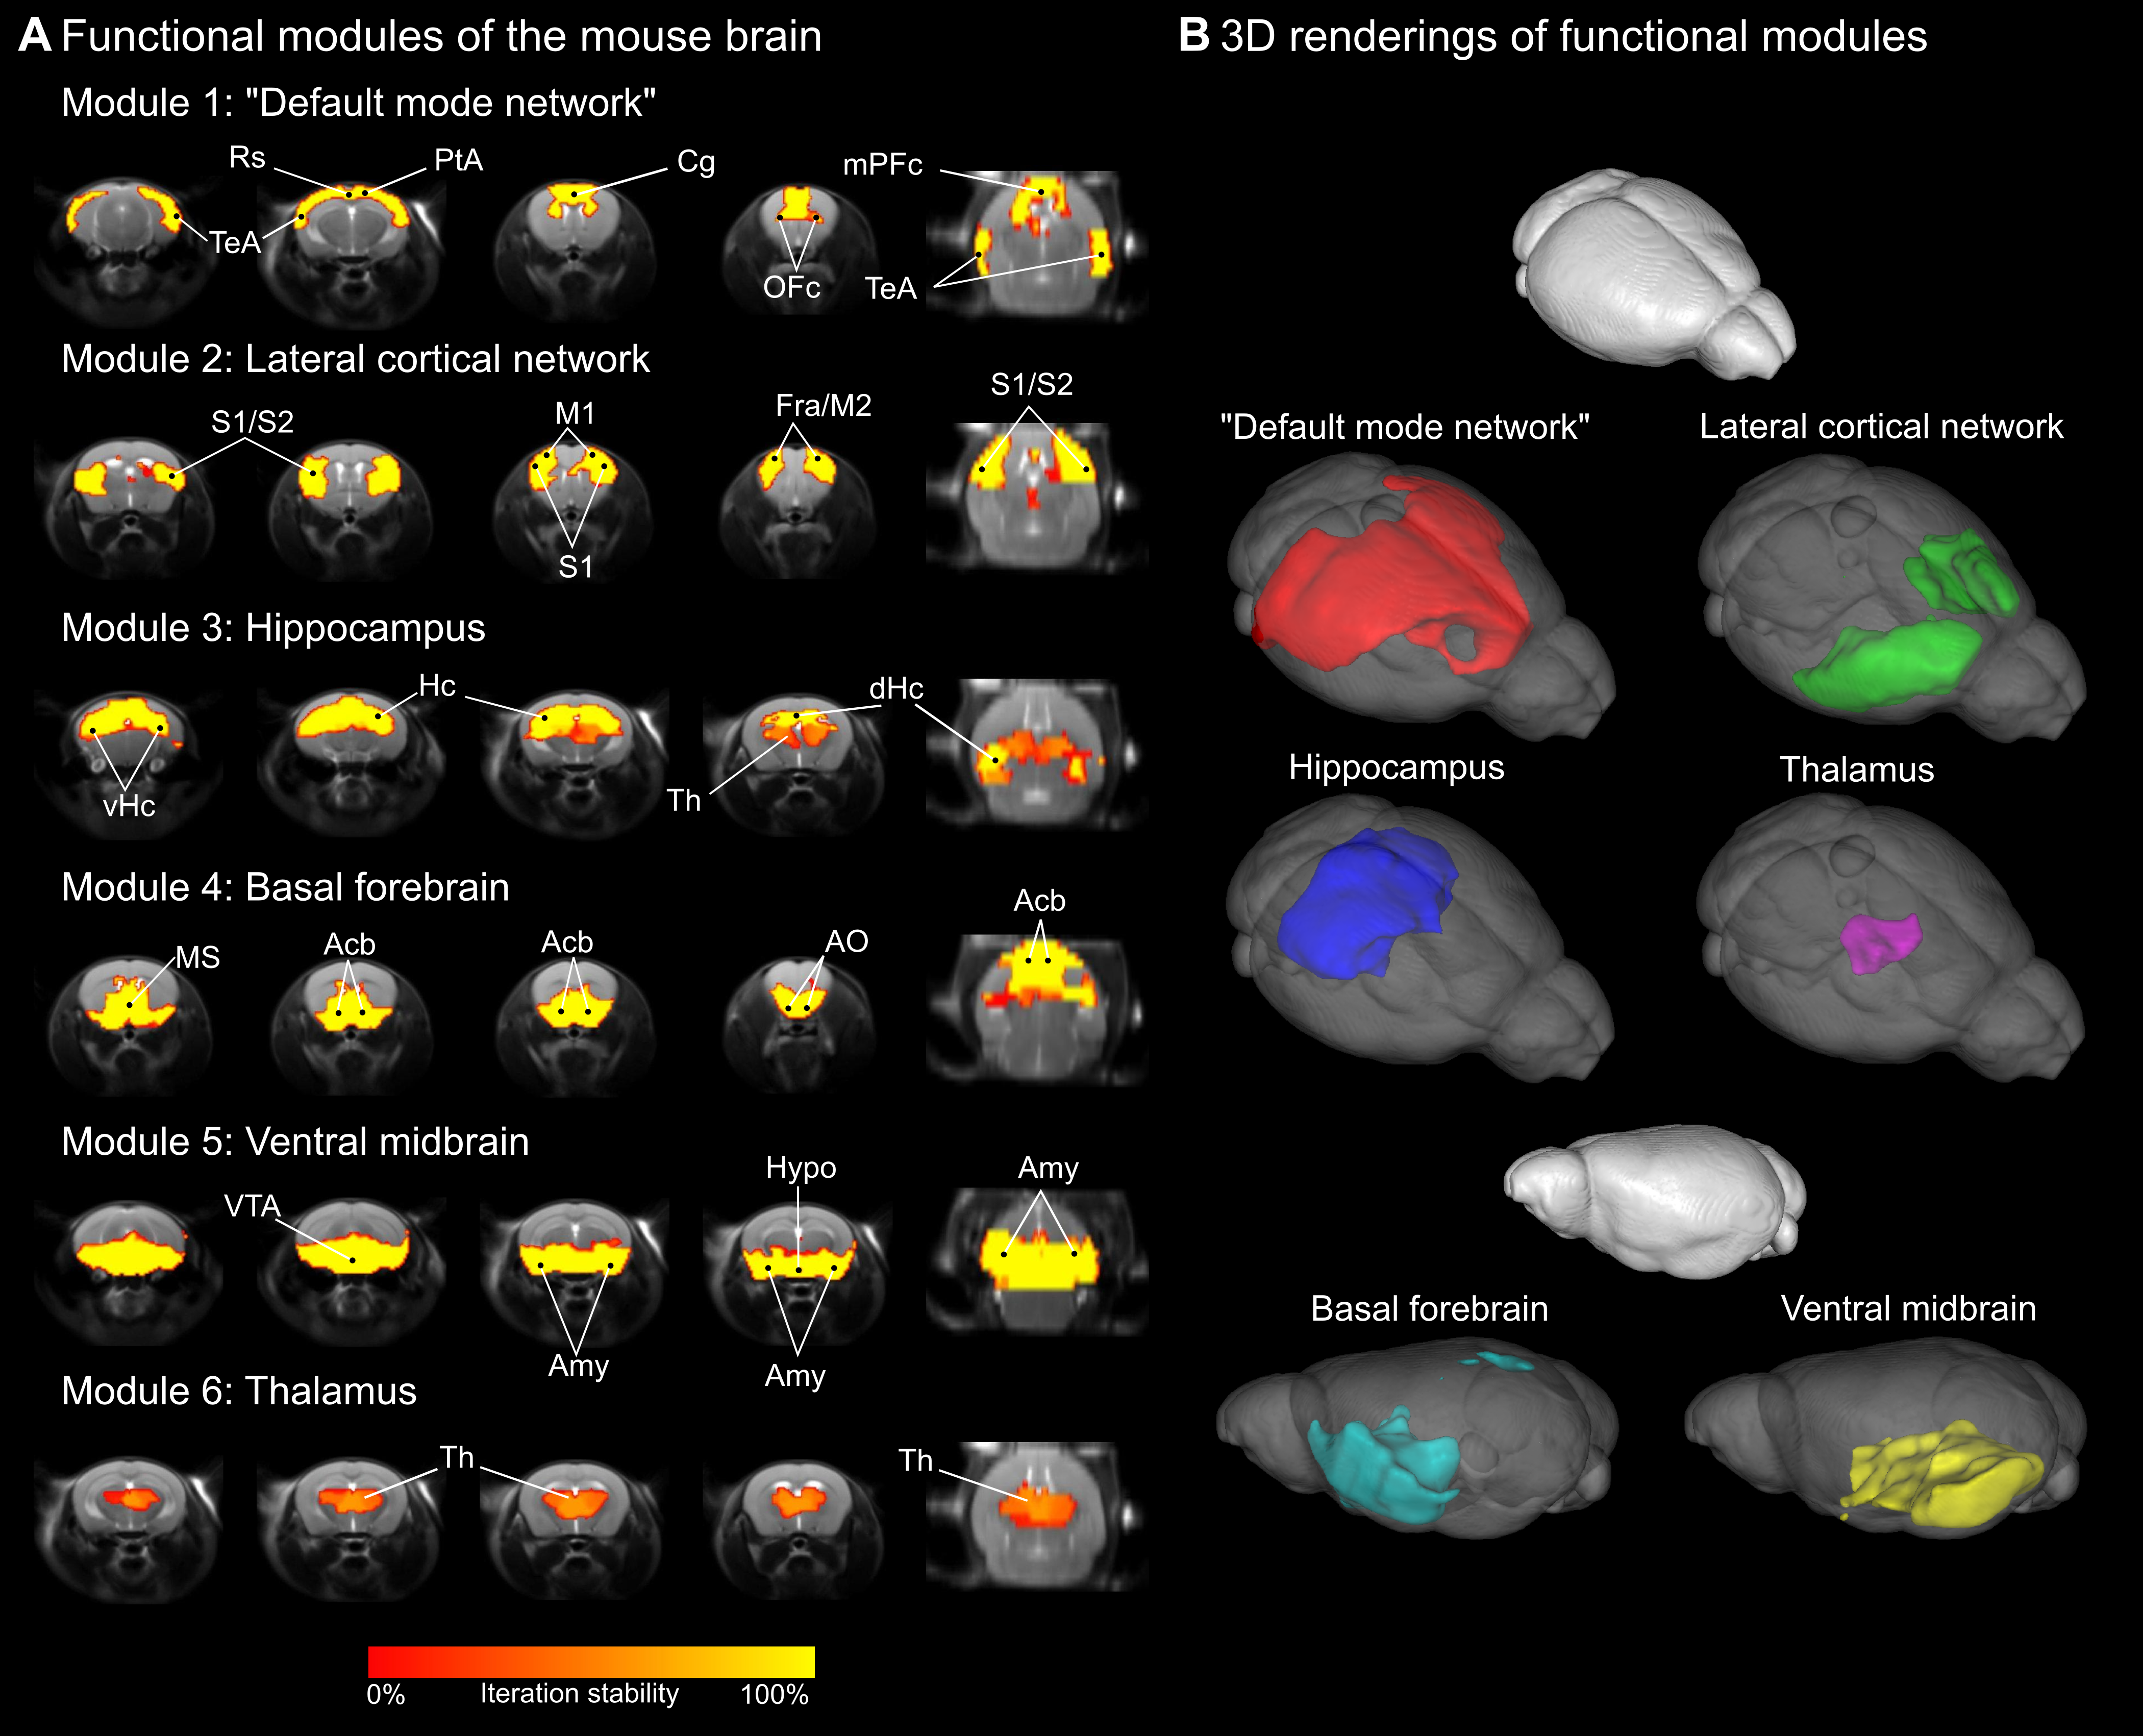
\includegraphics[scale=0.8]{figures/hubs_figure_01_modules_NEW.png}
    \decoRule
    \caption[Functional modules of the mouse brain.]{Functional modules of the
    mouse brain. (\textbf{A}) Module stability maps (100 iterations, N=41
    subjects) overlaid on the anatomical template. For each module, four
    representative coronal slices (left) and one image in the horizontal plane
    (right) are shown. (\textbf{B}) Three-dimensional renderings of the
    reference partition within a transparent brain template. Opaque renderings
    show brain orientation.}
    \label{fig:hubs_fig01_modules}
\end{figure}

\begin{figure}[th]
    \centering
    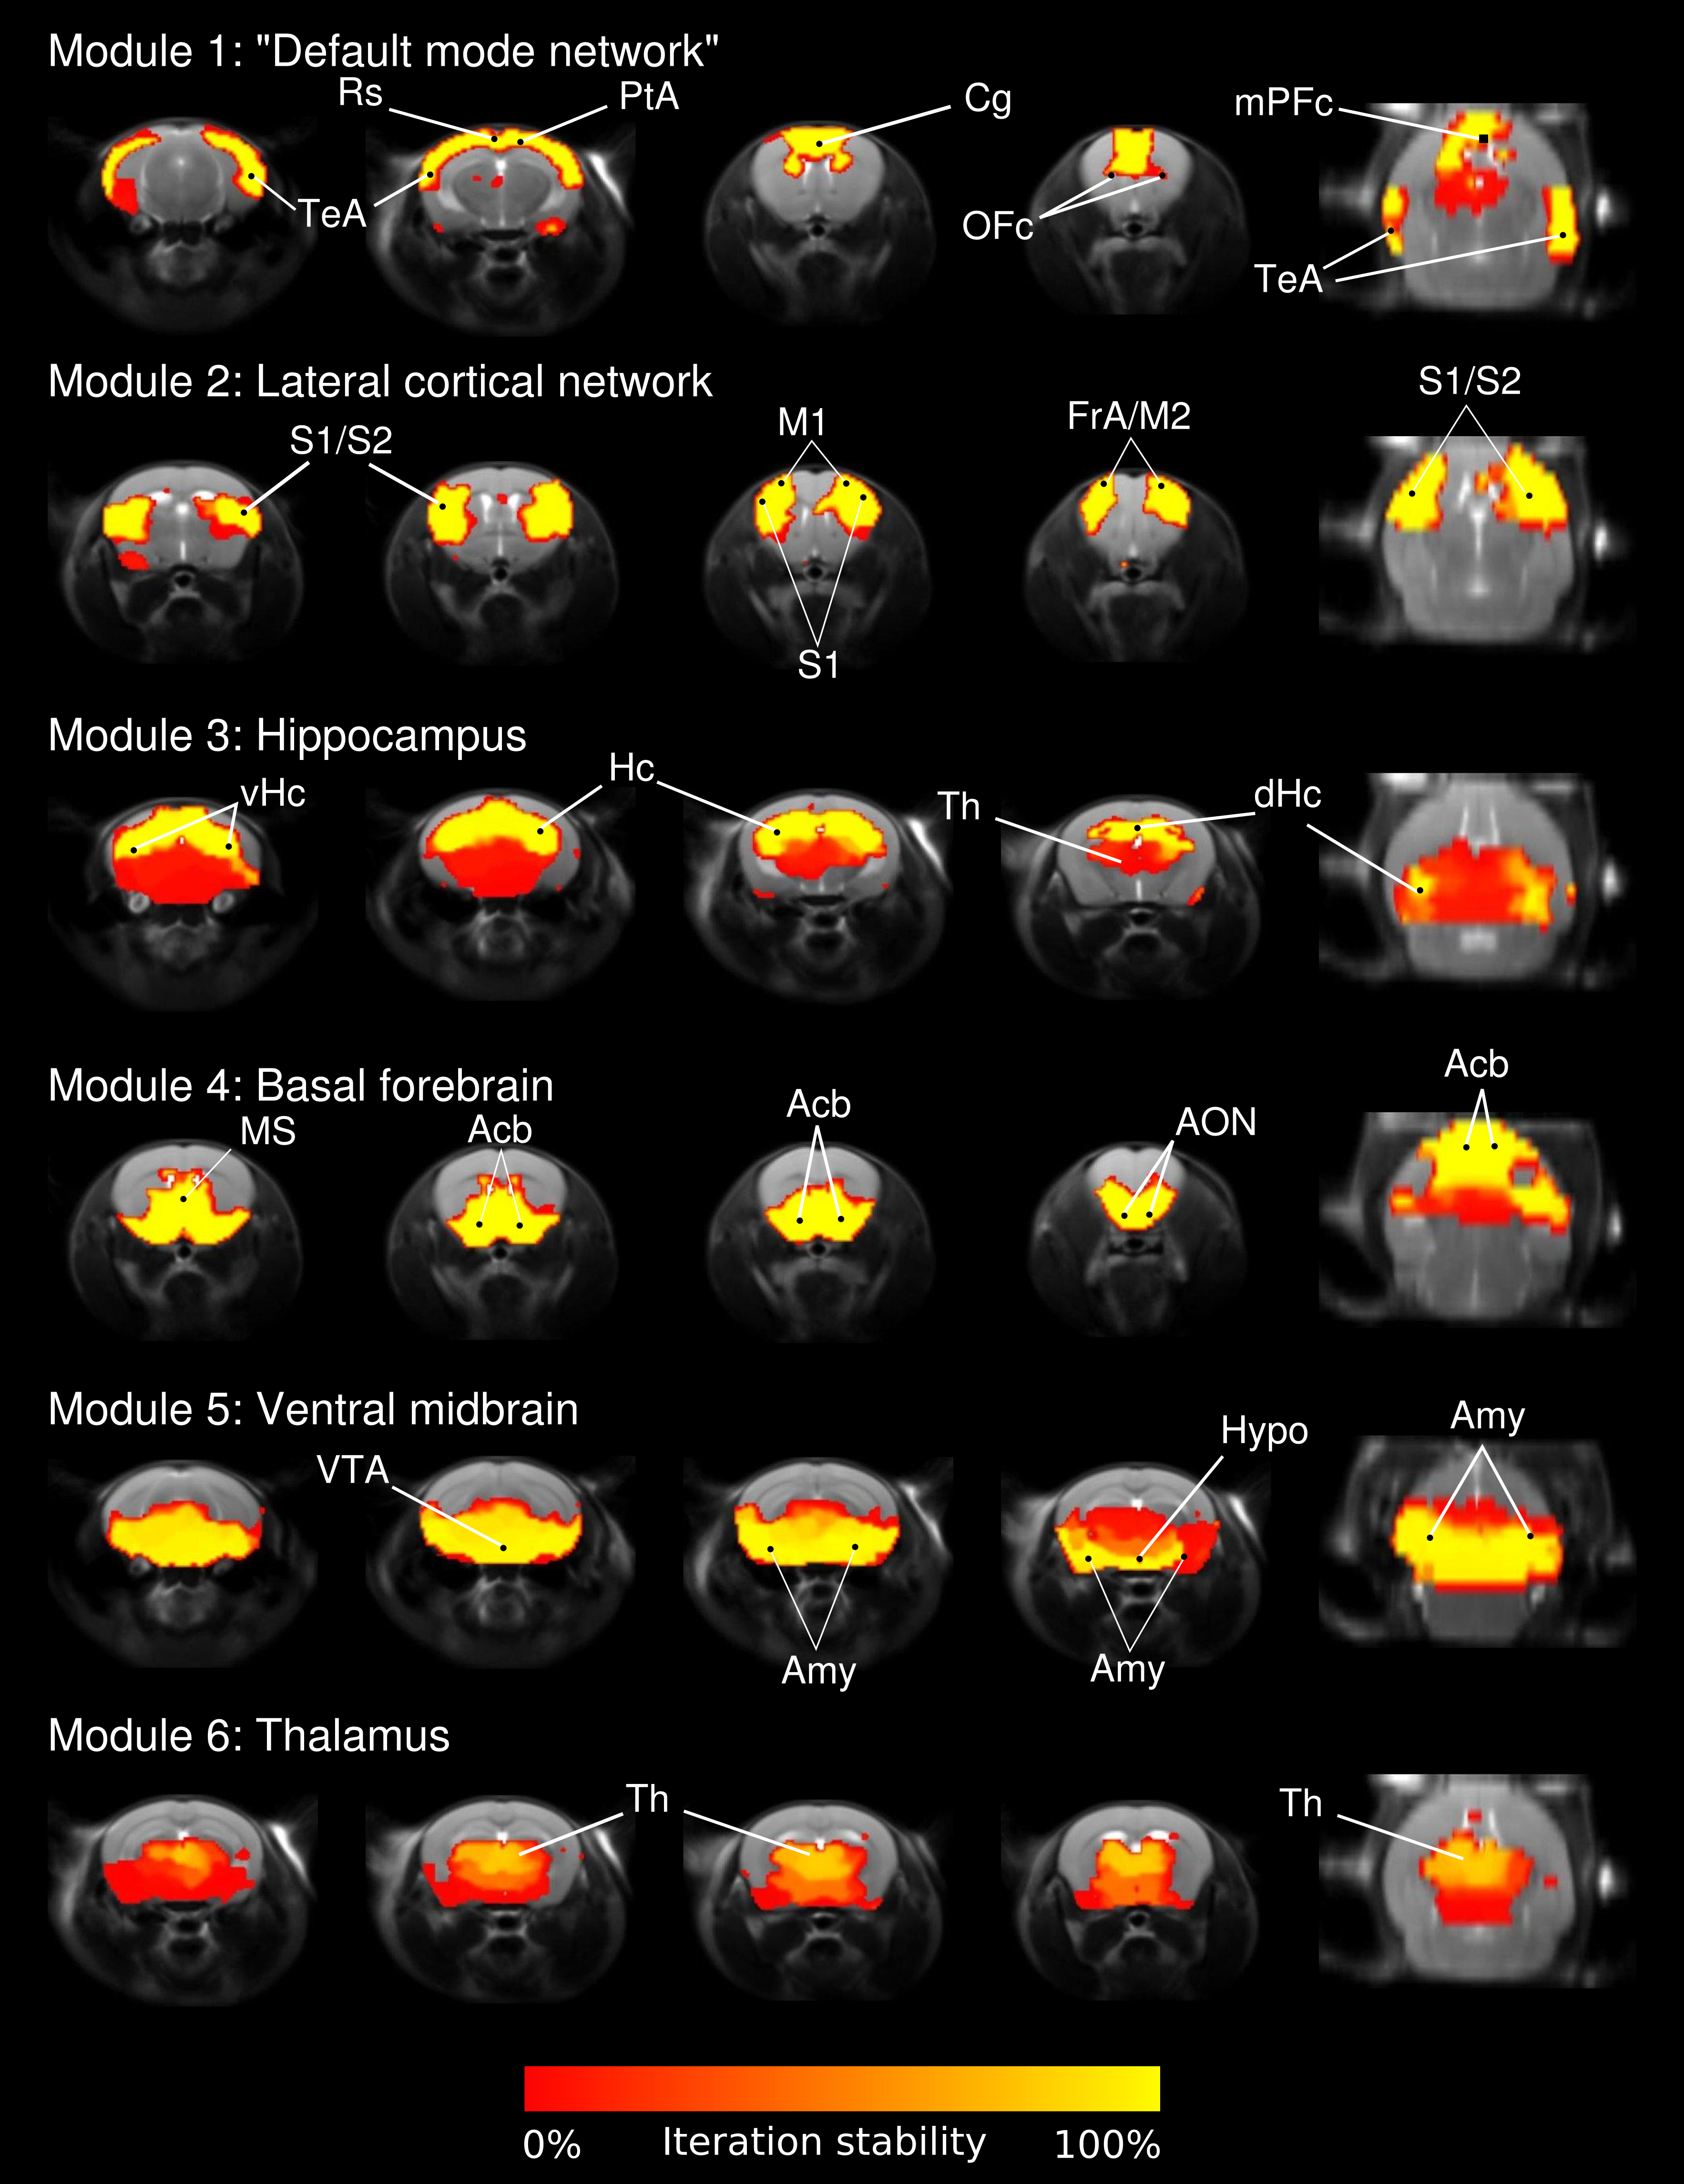
\includegraphics[scale=0.7]{figures/hubs_figure_s2_GSR_modules.png}
    \decoRule
    \caption[Functional modules of the mouse brain computed after global signal
    regression.]{Functional modules of the mouse brain computed after global
    signal regression. Module stability maps (100 iterations, N=41 subjects)
    overlaid on the anatomical template. For each module, four representative
    coronal slices (left) and one image in the horizontal plane (right) are
    shown.}
    \label{fig:hubs_figs2_gsr_modules}
\end{figure}

\begin{figure}[th]
    \centering
    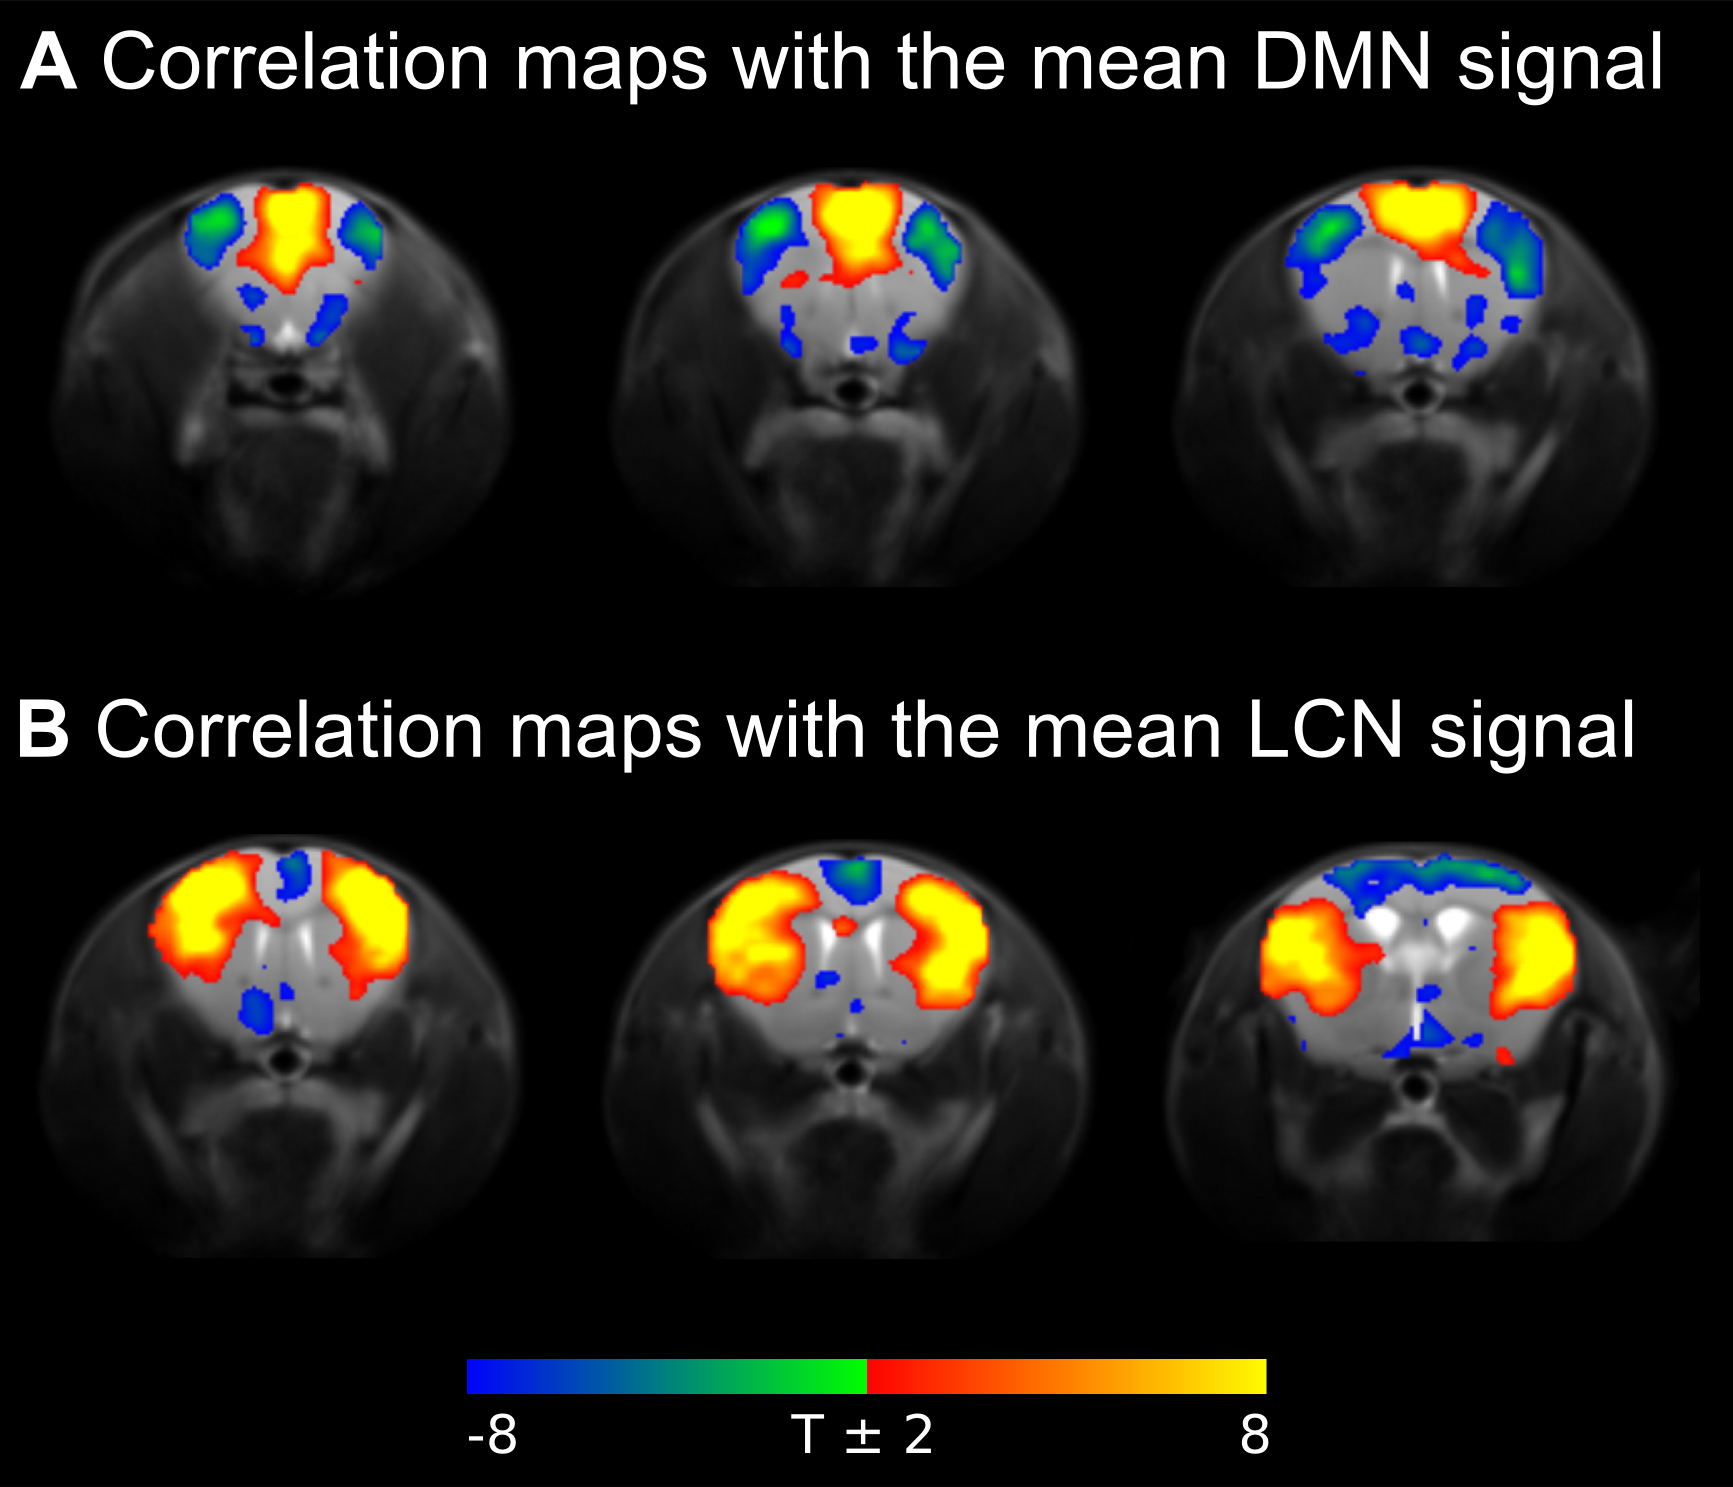
\includegraphics[scale=1]{figures/hubs_figure_s3_dmn_lcn_anticorr.png}
    \decoRule
    \caption[Anticorrelation between the time courses of the default mode and
    lateral cortical networks.]{The two cortical modules identified in the
    study, the default mode network (DMN) and lateral cortical network (LCN),
    are anticorrelated in the dataset with global signal regression.}
    \label{fig:hubs_figs3_anticorrelations}
\end{figure}

To further confirm the robustness of our modular partition, and rule out bias
from spatial smoothing and voxel adjacency artefacts \parencite{power2013} we
carried out a modular partition of functional network in which all connections
shorter than 0.5 mm (approximately 2.5 voxels in plane) were removed, leading to
the identification of a set of modules very consistent with those observed with
full network (Fig.~\ref{fig:hubs_figs4_short_connections}A). With a much more
stringent selection (i.e. removal of connections shorter than 1 mm, ca. 5 voxels
in plane) modular instability was observed for subcortical modules, with
evidence of stable partitioning of the DMN and thalamic modules as a single
joint community (Fig.~\ref{fig:hubs_figs4_short_connections}B). This modular structure is consistent with previous
seed-based rsfMRI studies of the mouse brain, in which thalamic areas appear to
be strongly correlated with cingulate and retrosplenial cingulate cortices
\parencite{sforazzini2016}. The appearance of subcortical modular instability
upon removal of 1 mm connections is not unexpected, because 1 mm long
connections cover the anatomical extension of some of the anatomical structures
that constitute individual functional modules (e.g.  radial hippocampus, or
thalamus) \parencite{paxinos2004}. 

\begin{figure}[th]
    \centering
    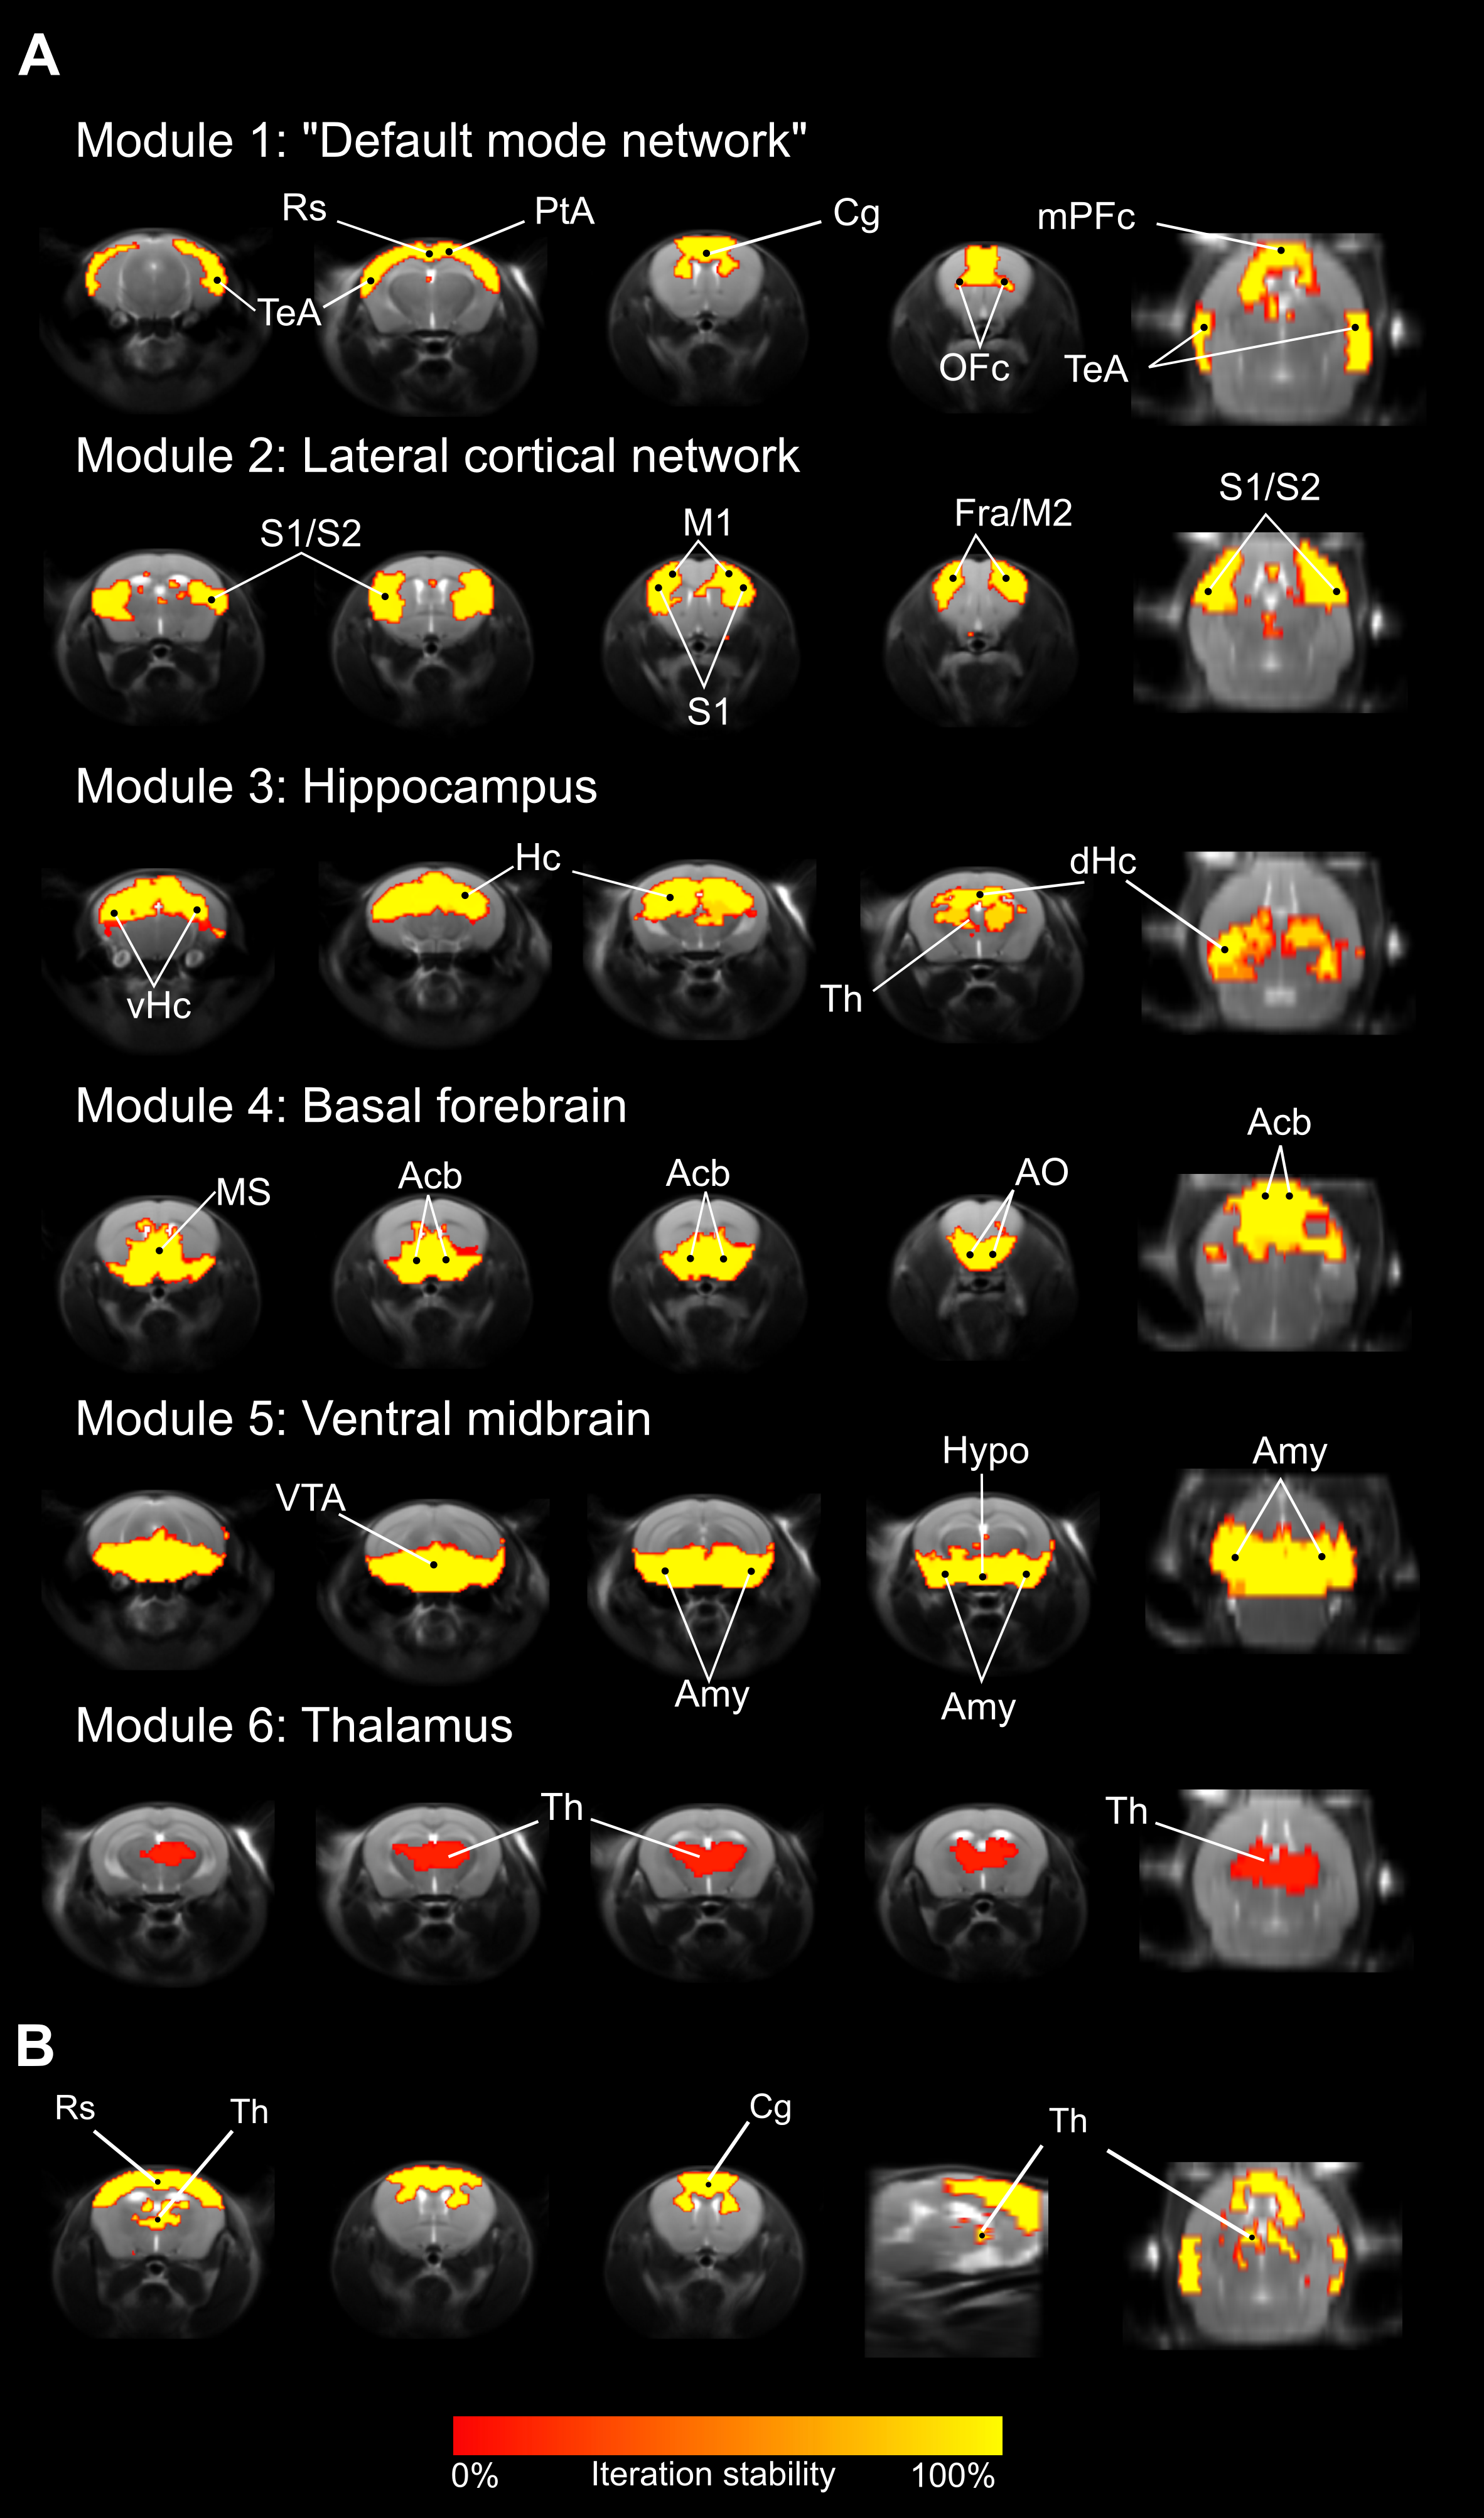
\includegraphics[scale=0.85]{figures/hubs_figure_s4_modules_short_edges_removed.png}
    \decoRule
    \caption[Modules of the mouse brain upon removal of short
    connections.]{Modules of the mouse brain upon removal of short connections.
    (\textbf{A}) Connections shorter than 0.5 mm were removed. (\textbf{B}) DMN
    module in the functional network upon removal of connections shorter than
    1.0 mm. Module stability maps (100 iterations, N=41 subjects) are overlaid
    on the anatomical template.}
    \label{fig:hubs_figs4_short_connections}
\end{figure}


\subsection{Global functional hubs are located in cingulate and prefrontal
cortex}

To identify functional hubs at a voxel scale, we first mapped connection
strength values for all nodes in the functional network \parencite{rubinov2011}.
In agreement with human studies \parencite{tomasi2011}, cortical and subcortical
regions appeared to have distinct connectional profiles, with the former
exhibiting much higher strength overall (Fig.~\ref{fig:hubs_fig2_global_hubs}A).
Anatomical maps of the voxels exhibiting the highest strength ($p < 0.0001$, FDR
corrected) revealed foci of high connection strength in several sub-regions of
the DMN network, including prefrontal, anterior and posterior cingulate cortex
as well as parietal association regions (Fig.~\ref{fig:hubs_fig2_global_hubs}B). 

\begin{figure}[th]
    \centering
    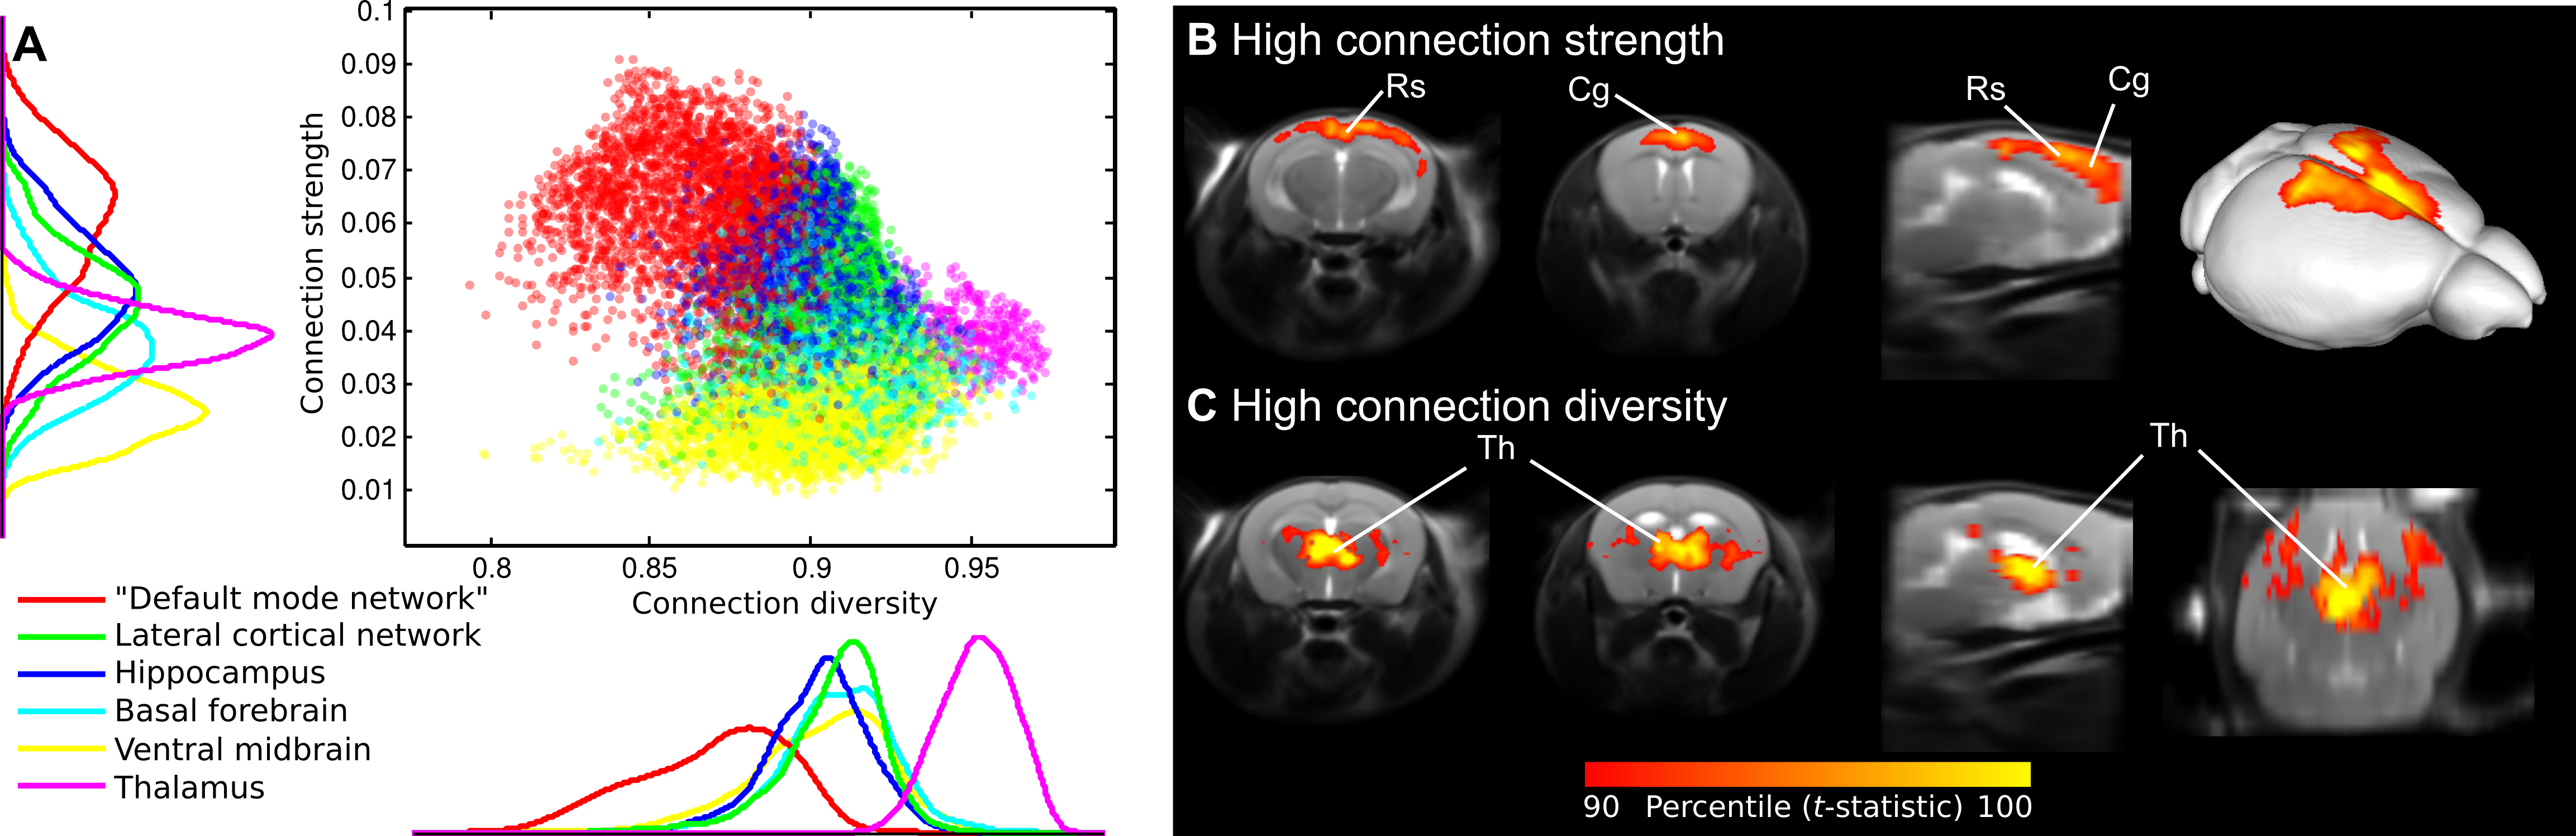
\includegraphics[scale=0.7]{figures/hubs_figure_02_hubs_global_NEW.png}
    \decoRule
    \caption[Global hubs of the mouse brain.]{Global hubs of the mouse brain.
    (\textbf{A}) Connection diversity and connection strength values are plotted
    for all nodes in the average functional network. Nodes are colour-coded
    according to their module. (\textbf{B}) Nodes surviving the top percentage
    threshold for connection strength are shown on two images in the coronal
    view (left), one image in the sagittal view (middle), and on a
    three-dimensional cortical surface rendering. (\textbf{C}) Nodes surviving
    the top percentage threshold for connection diversity are shown on two
    images in the coronal view, one image in the sagittal view (left), one image
    in the sagittal view (middle), and on a three-dimensional cortical surface
    rendering.}
    \label{fig:hubs_fig2_global_hubs}
\end{figure}


To account for potential bias induced by coil-induced regional variation in
temporal signal to noise ratio (tSNR), we performed connection strength mapping
on rsfMRI timeseries corrupted with random pink noise such to achieve homogenous
tSNR levels equalling values observed in deep subcortical areas ($\approx 25$).
The results of this analysis confirmed the original hub locations ($p < 0.0038$,
FDR corrected, Fig.~\ref{fig:hubs_figs5_snr}) thus ruling out a significant
contribution of coil-related bias on high strength connection maps.

\begin{figure}[th]
    \centering
    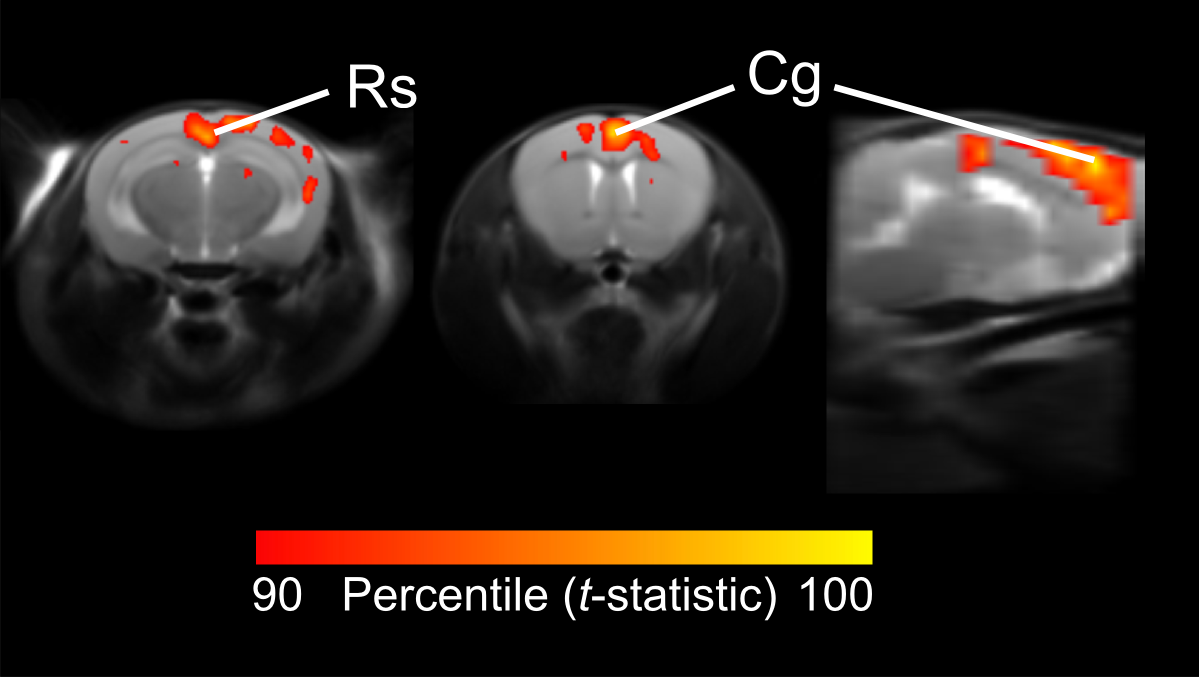
\includegraphics[scale=1.2]{figures/hubs_figure_s5_snr.png}
    \decoRule
    \caption[High-strength nodes in rsfMRI time series after tSNR corruption
    with pink noise.]{High-strength nodes in rsfMRI time series after tSNR
    corruption with pink noise. The final timeseries had tSNR values similar to
    those observed in deep brain areas furthest to the surface coil array
    ($\approx 25$).  In spite of this, cingulate and retrosplenial areas emerged
    as regions with highest global connectivity strength.}
    \label{fig:hubs_figs5_snr}
\end{figure}

\subsection{High connection diversity hubs are located in the thalamus and
associative cortical areas}

Connection diversity is a network attribute used to identify nodes participating
in multiple functional sub-networks \parencite{power2013, rubinov2011}.
Whole-brain mapping of nodes exhibiting high connection diversity ($p < 0.001$,
FDR corrected) revealed a prominent involvement of thalamic areas
(Fig.~\ref{fig:hubs_fig2_global_hubs}A,C), a finding consistent with the
integrative and relay functions subserved by this region
\parencite{draganski2008}. 

To extrapolate and compare our results with human studies, where topological
analyses are typically limited to cortical regions, we also generated a map of
high connection diversity voxels within the identified neocortical modules
(Fig.~\ref{fig:hubs_fig3_cortical_hubs}). As recently described in humans
\parencite{power2011}, nodes within the DMN module exhibited low average
connection diversity, suggesting an extensive internal integration of this
module and its function as a highly efficient “processing” system. Importantly,
the approach also led to the identification of spatially restricted foci of high
connection diversity the temporal association cortex ($p < 0.001$, FDR corrected),
a cortical area serving prominent integrative roles. Consistent with recent
human studies \parencite{power2013}, foci of high connection diversity were also
found in the anterior insular cortex ($p < 0.032$, uncorrected), although in this
region the effect appeared to be less robust and did not survive FDR correction
($p < 0.2905$, FDR corrected).

\begin{figure}[th]
    \centering
    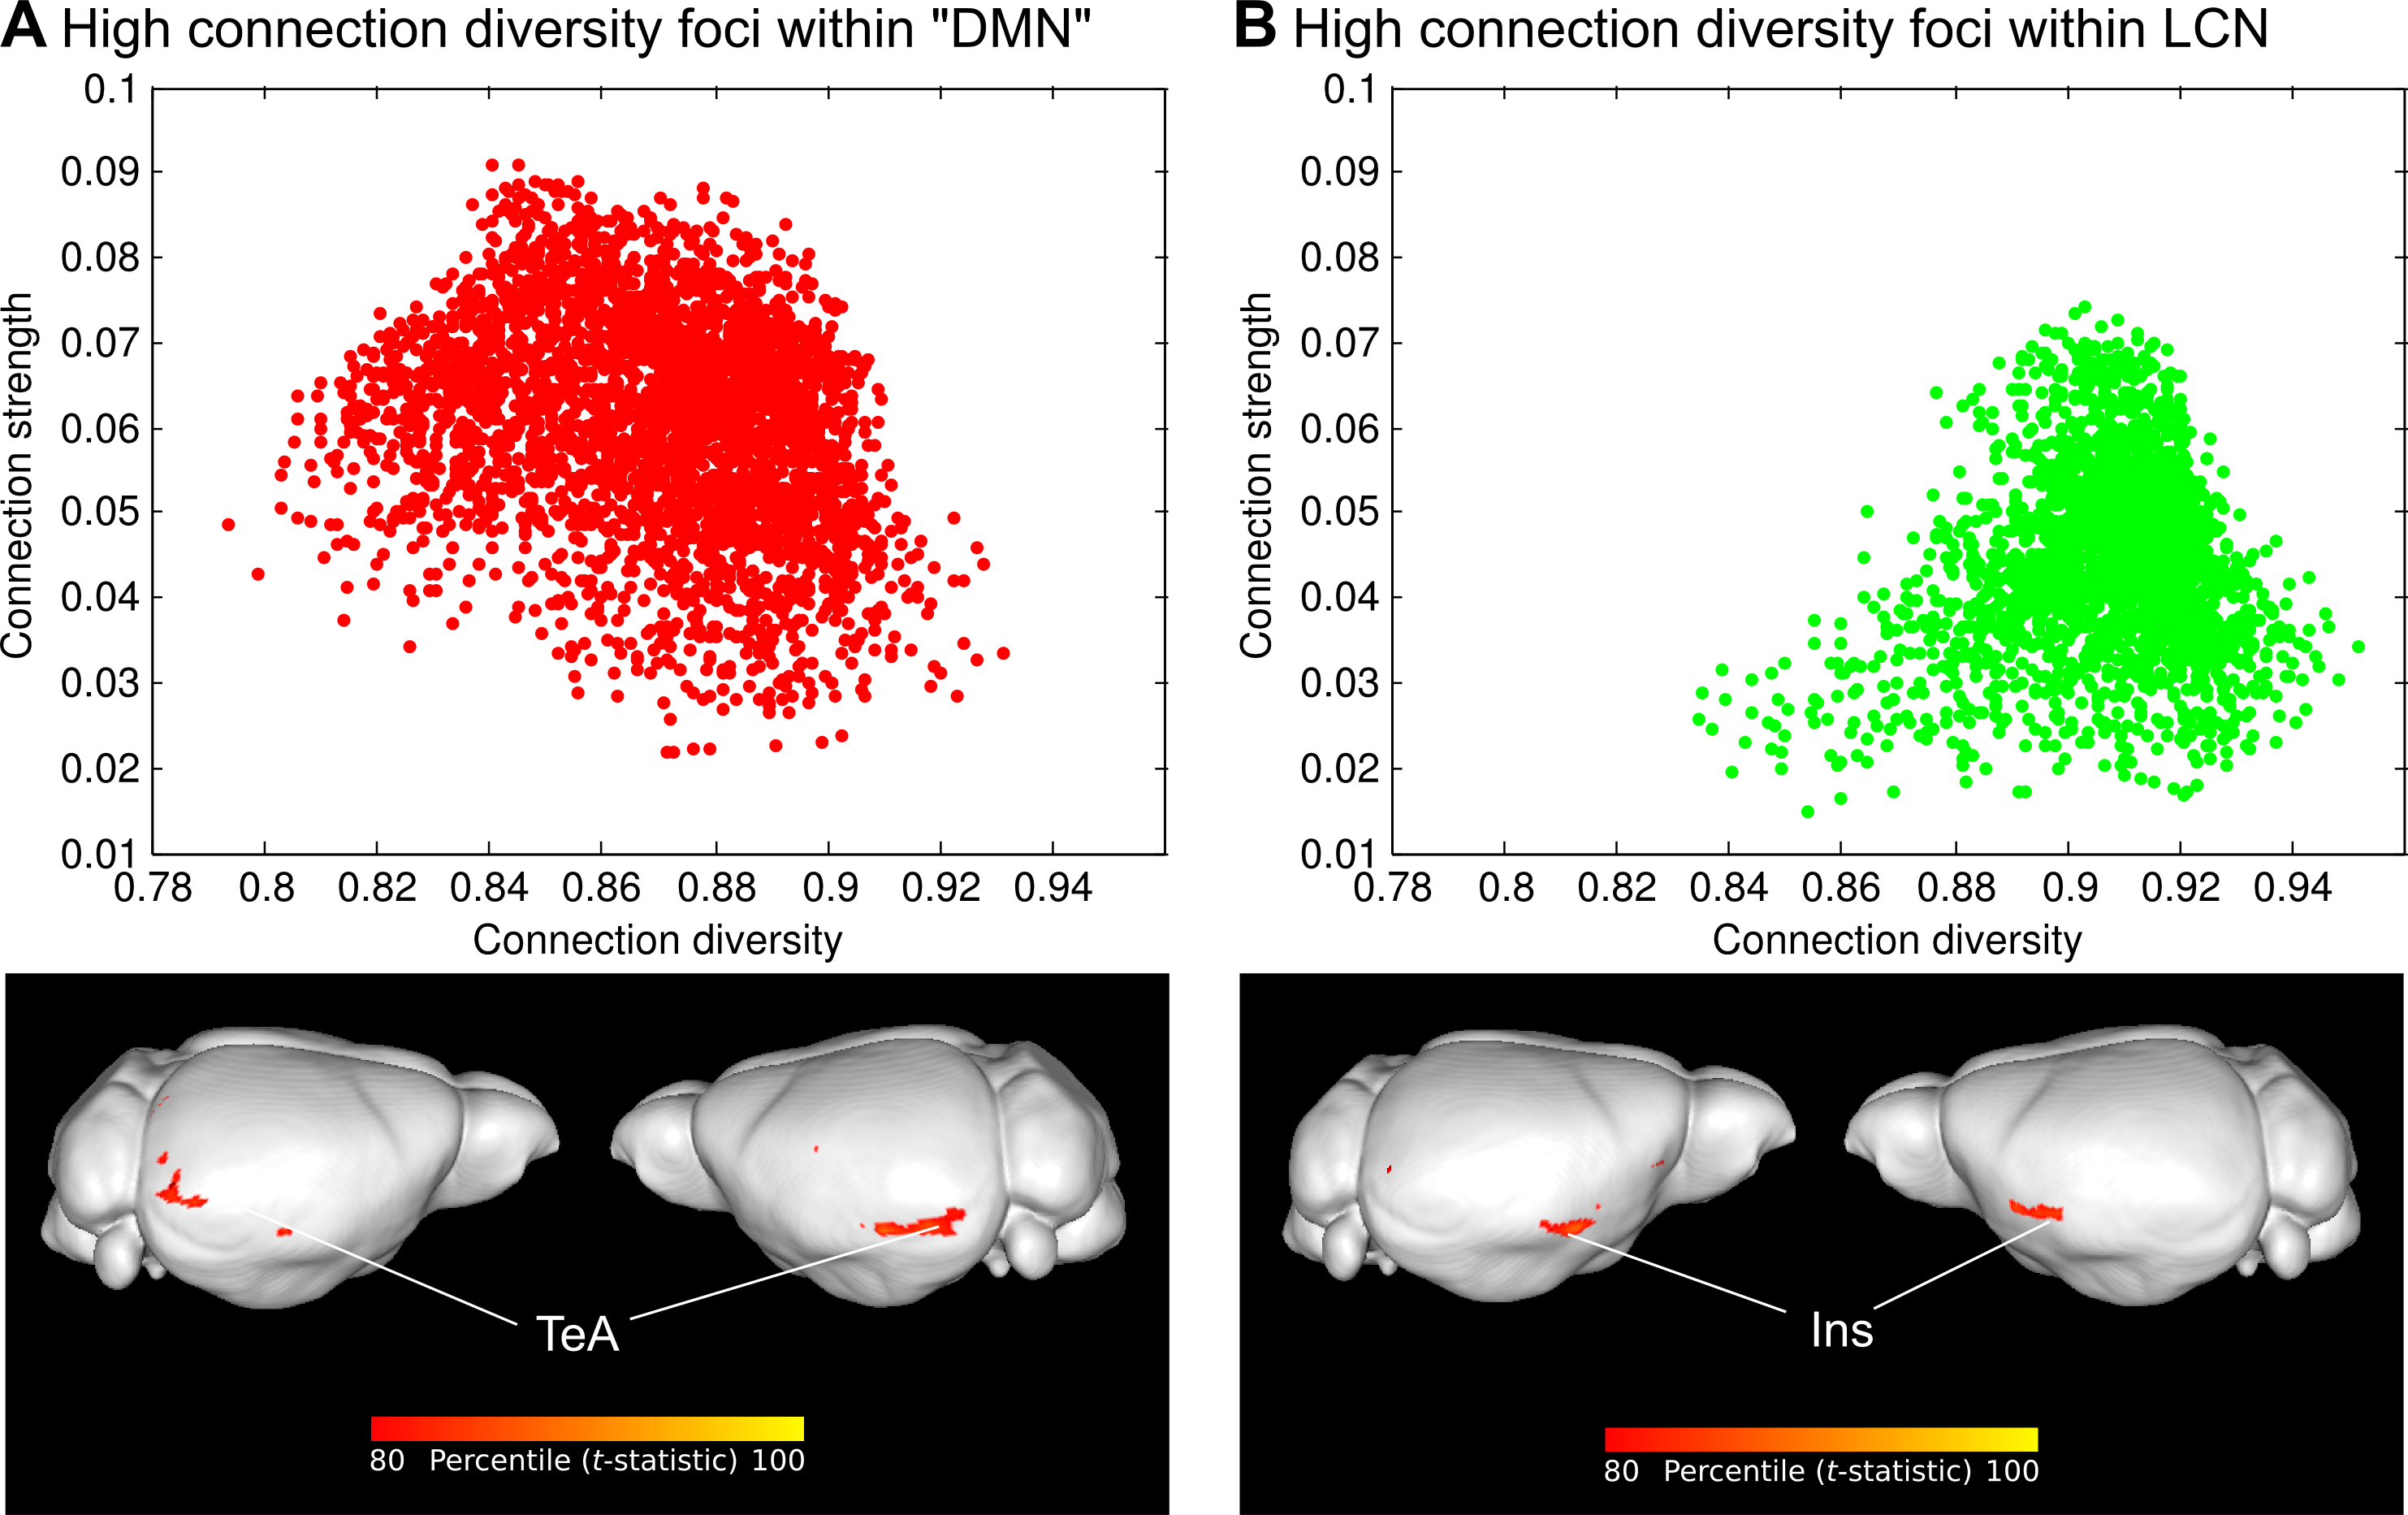
\includegraphics[scale=1.1]{figures/hubs_figure_03_cortical_hubs_NEW.png}
    \decoRule
    \caption[High connection diversity regions within cortical modules.]{High
    connection diversity regions within cortical modules. Connection diversity
    and strength values (calculated in the average functional network) are
    plotted for all nodes in the “default mode network” (\textbf{A}) and the
    lateral cortical network (\textbf{B}). Bottom panels highlight brain nodes
    surviving the top percentage threshold within each of the two cortical. The
    nodes are shown as three dimensional renderings on the cortical surface.}
    \label{fig:hubs_fig3_cortical_hubs}
\end{figure}

\subsection{Intra-module mapping of high connection hubs}

To further investigate the topological organization of the individual
sub-networks, we mapped, for each of the identified modules, voxels
characterised by high within-module connectivity strength, which we refer to as
“module hubs” (Fig.~\ref{fig:hubs_fig4_module_hubs}). The top 10 \% voxels were
statistically highly significant for all the modules, with the exception of the
ventral midbrain module, where the FDR corrected p-value was, however, very
close to significance level (DMN: $p < 0.000011$, LCN: $p < 0.00039$, Hc: $p <
0.0016$, basal forebrain: $p < 0.0068$, ventral midbrain: $p < 0.0572$, thalamus: $p <
0.0000096$, all FDR corrected). Module hub mapping in the DMN and lateral
cortical networks highlighted high within-module strength foci in the anterior
cingulate cortex, and frontal association cortices, respectively. Additional
candidate module hubs were identified in the dorsal hippocampus (hippocampal
module), nucleus accumbens and olfactory nuclei (basal ganglia), pons/ventral
subiculum (ventral midbrain), and centromedial thalamic nuclei (thalamus). 

\begin{figure}[th]
    \centering
    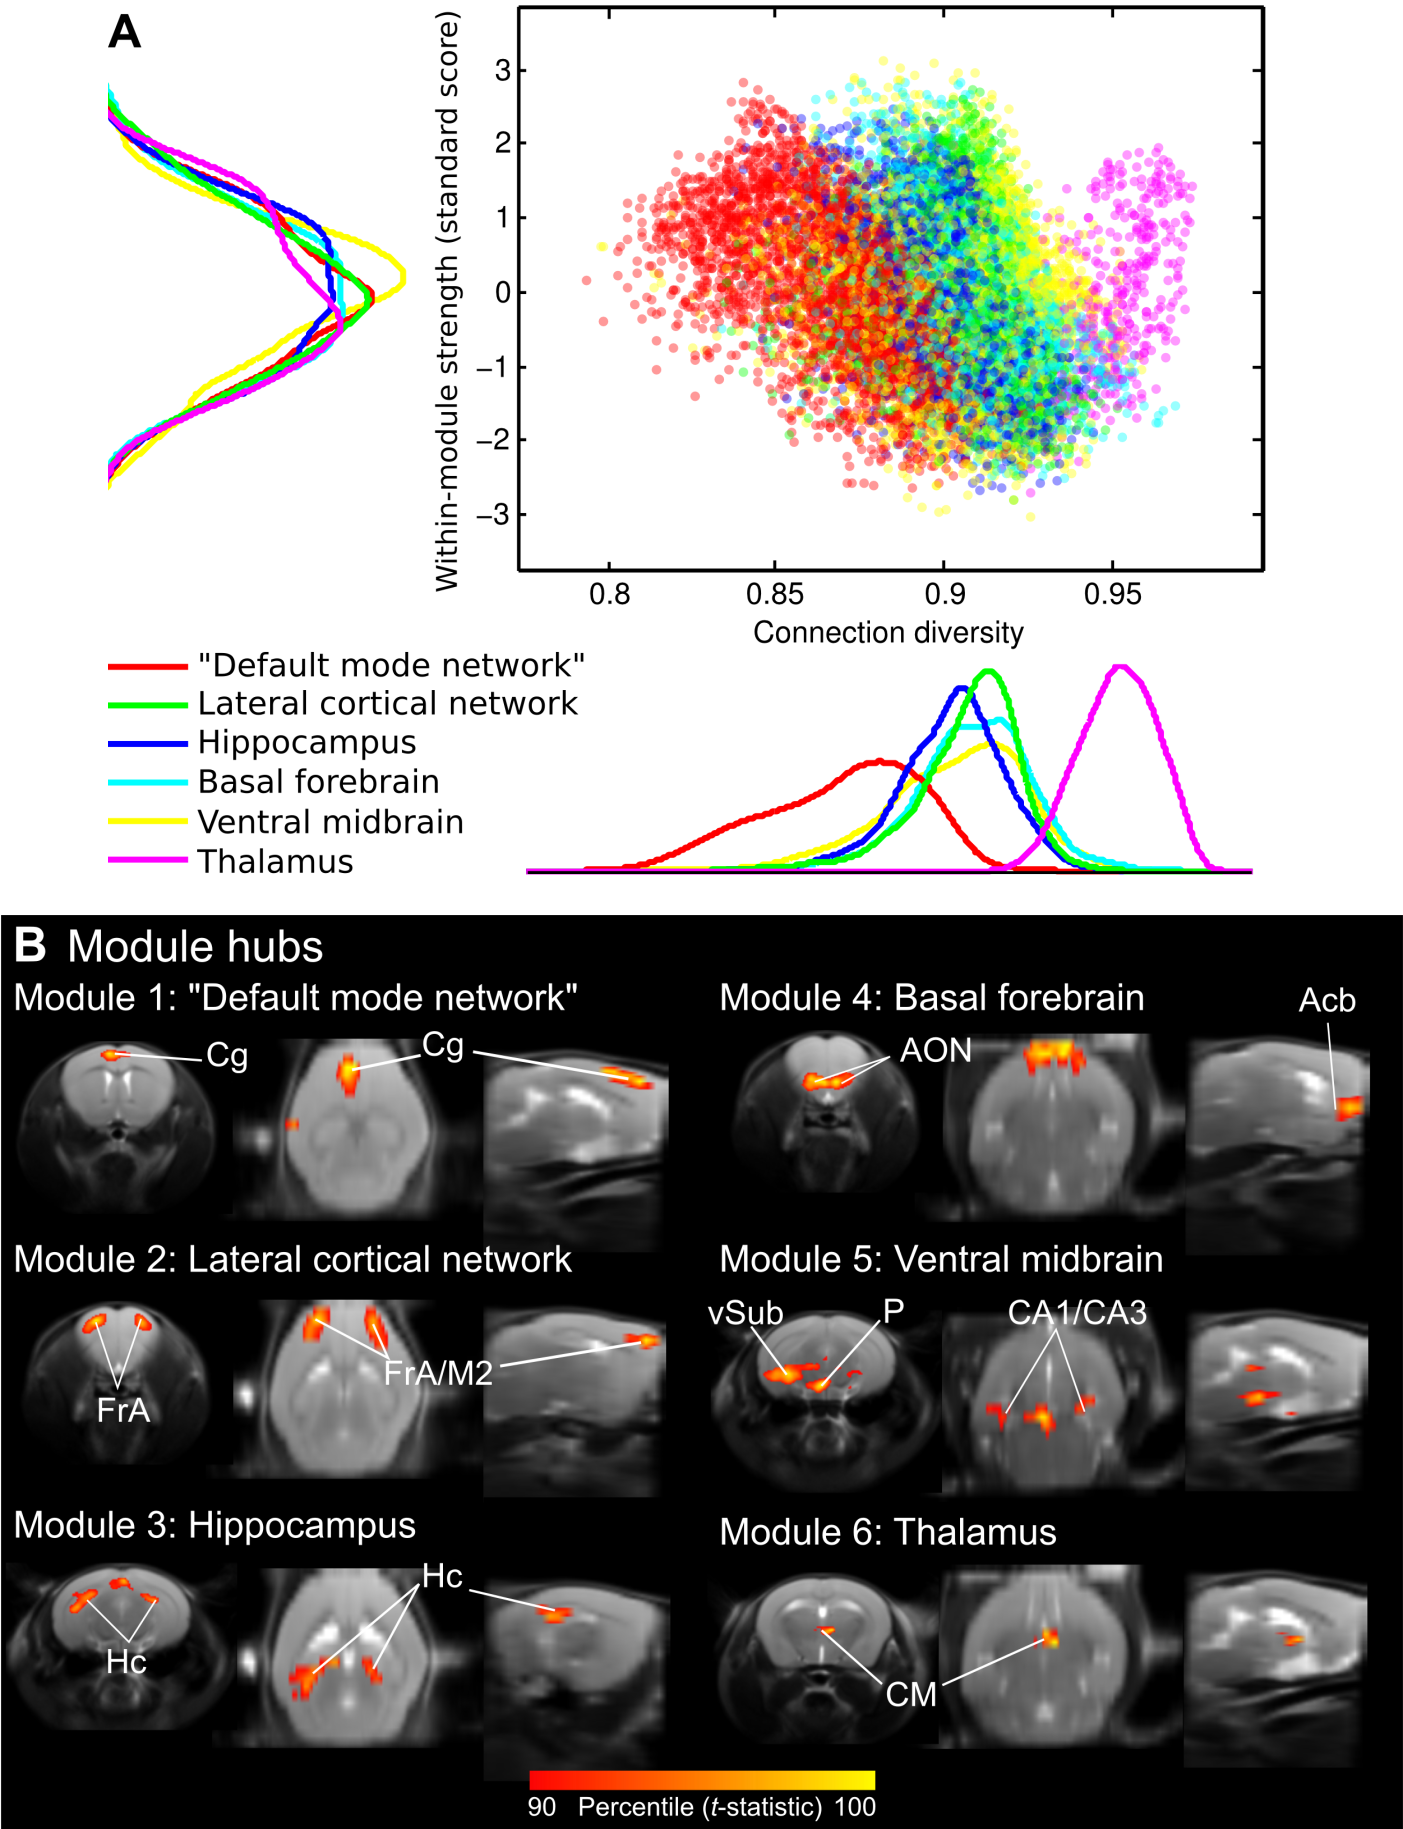
\includegraphics[scale=0.6]{figures/hubs_figure_04_module_hubs_NEW.png}
    \decoRule
    \caption[Module hubs.]{Module hubs. (\textbf{A}) Connection diversity and
    normalised (z) scores of within-module strength plotted for all nodes in the
    average functional network. Nodes are colour-coded according to their
    module.  (\textbf{B}) For each module, nodes surviving the top percentage
    threshold are shown on images in representative axial, horizontal and
    sagittal views of the mouse brain.}
    \label{fig:hubs_fig4_module_hubs}
\end{figure}

\subsection{Reproducibility of global and intra-module hub mapping on smaller
subject cohorts}

In order to evaluate the reproducibility of global and intra-module hub mapping
on smaller subject cohorts, 100 random subject subsets each with exactly N=10
animals were generated, and global and intra-module hub regions were mapped
independently for each group. The results show robust conservation of most hub
locations across the vast majority of randomly-generated 10-subject groups for
global and module hubs (Fig.~\ref{fig:hubs_figs6_reproducibility}). Diversity
hubs within the two cortical modules exhibited lower conservation, reflecting
intrinsic lower stability and significance levels these integrative locations as
reported above. 

\begin{figure}[th]
    \centering
    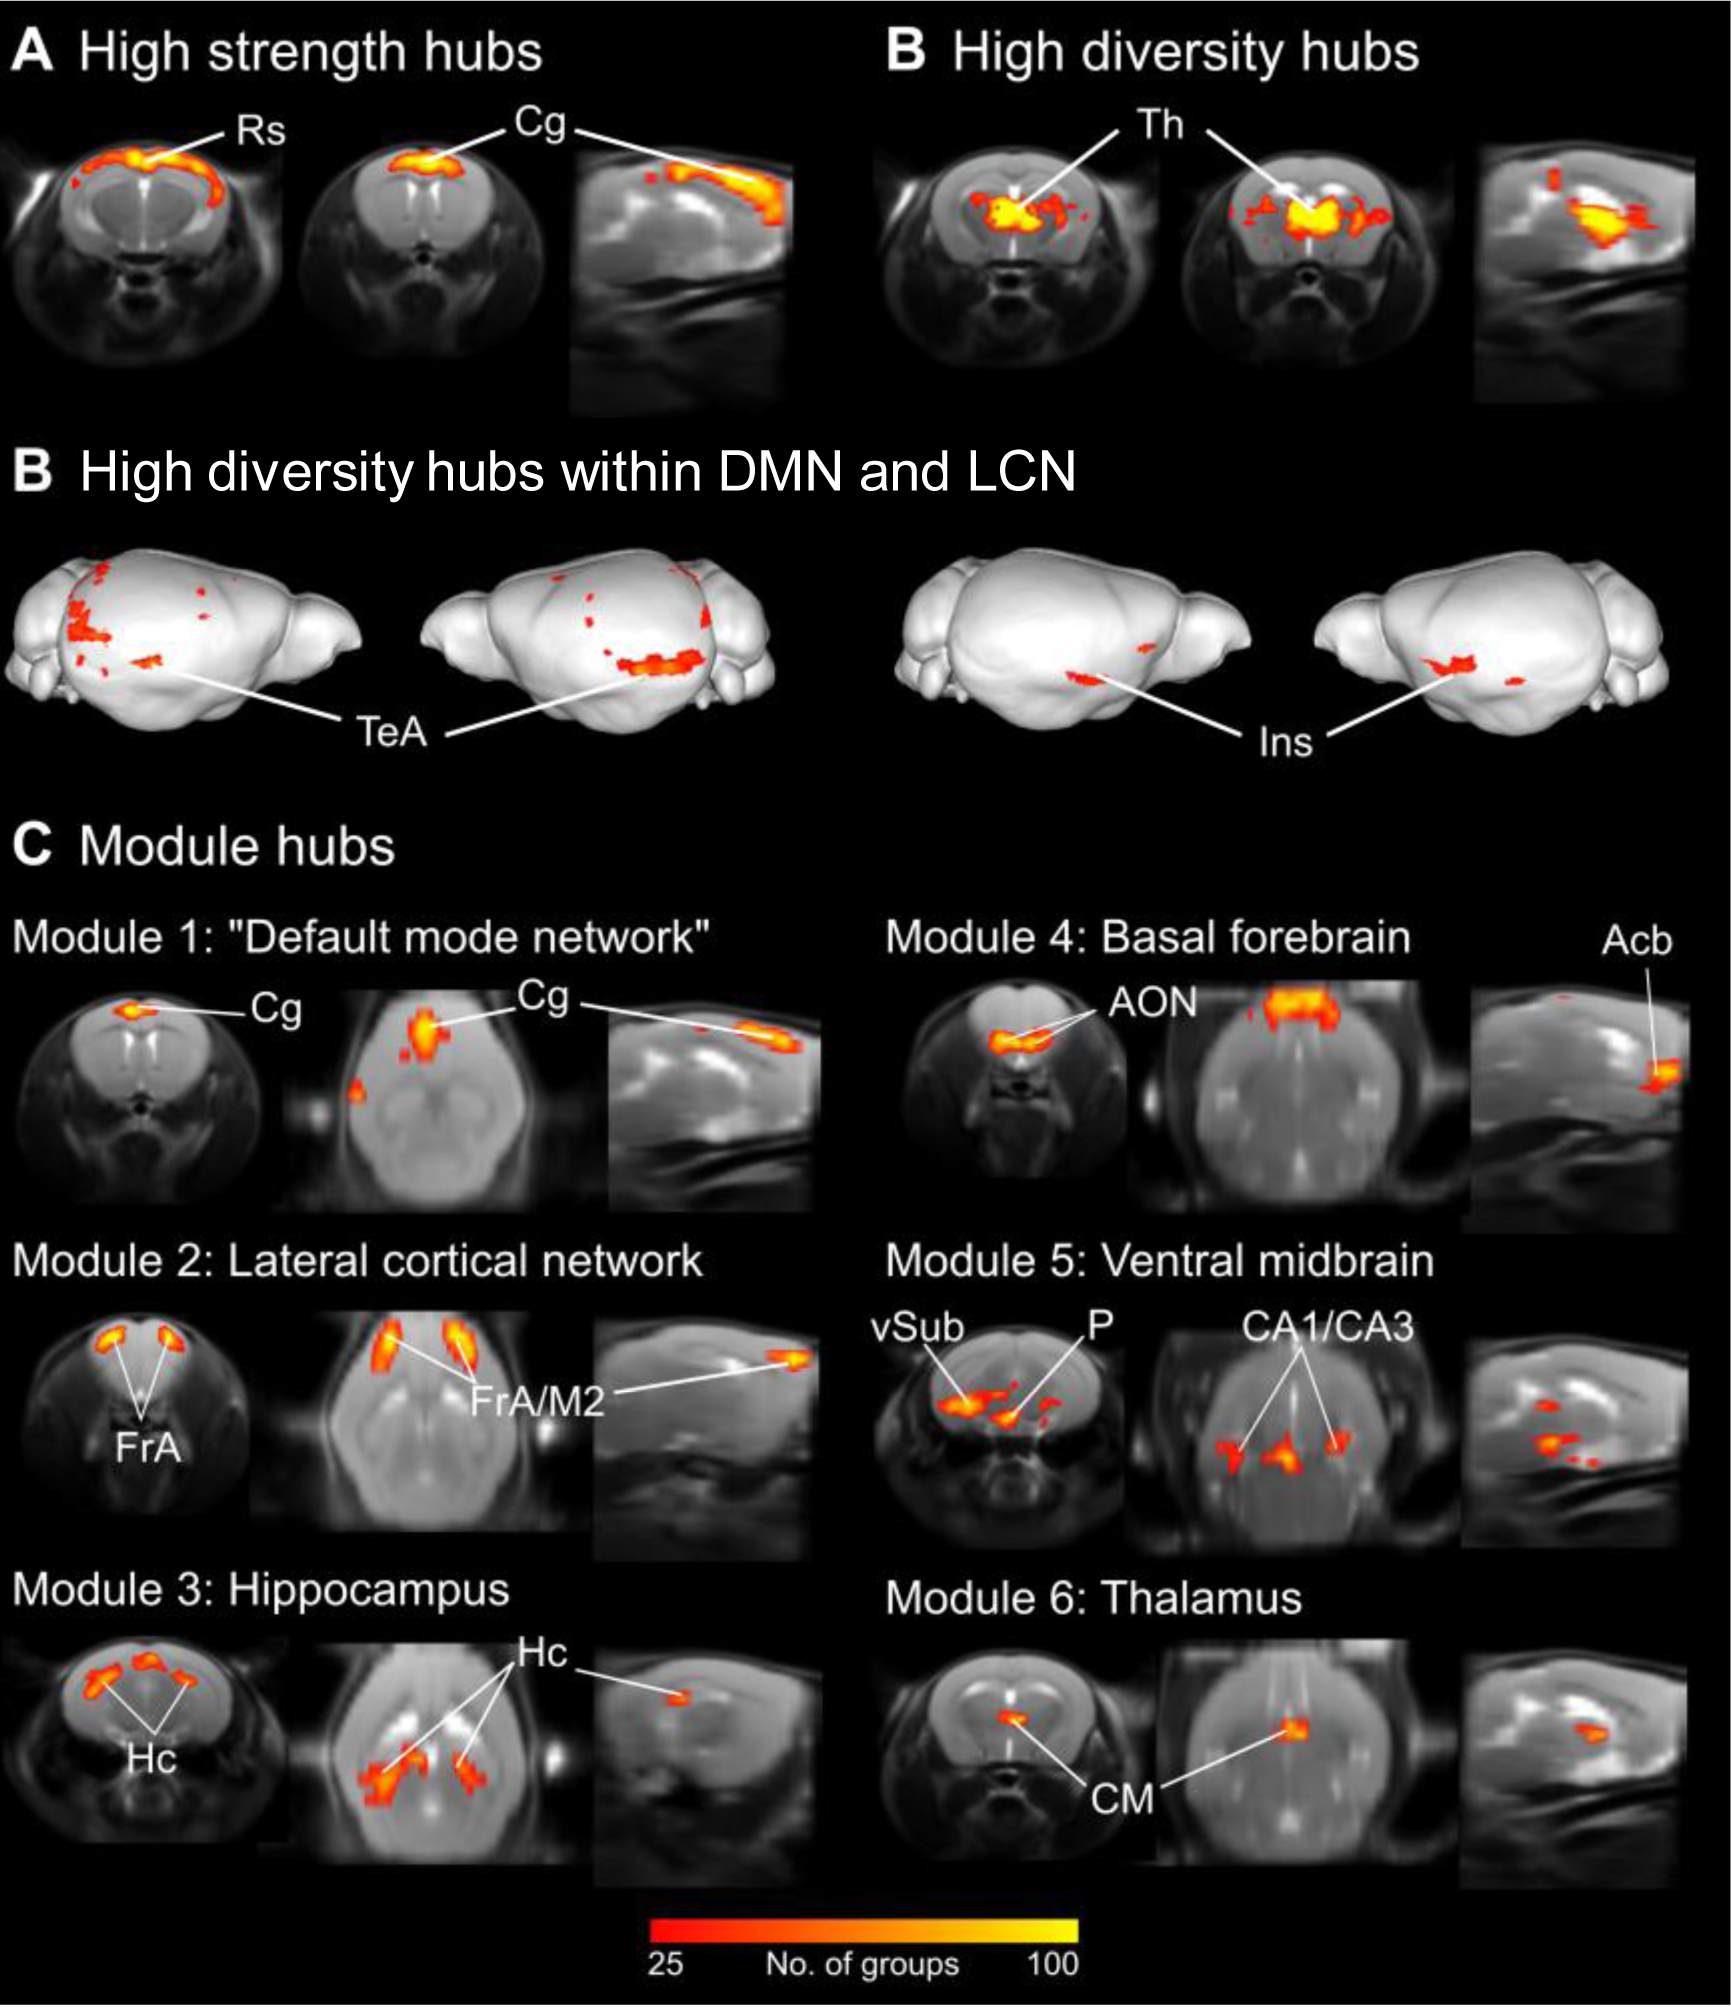
\includegraphics[scale=0.8]{figures/hubs_figure_s6_hub_reproducibility_10_animals_NEW.png}
    \decoRule
    \caption[Reproducibility of functional hubs in random sub-groups of 10
    animals.]{Reproducibility of functional hubs in random sub-groups of 10
    animals. The voxel maps express the number of groups (out of 100 random
    10-animal partitions of the original 41-subject cohort) in which a given
    voxel was identified as belonging to a hub of the given type.}
    \label{fig:hubs_figs6_reproducibility}
\end{figure}

\subsection{The identified hubs are mutually and preferentially interconnected}

To assess the presence of mutual inter-module connections between the identified
hubs, the anatomical correspondence between the strongest connections of each
source hub seed (Fig.~\ref{fig:hubs_figs1_seed_location}) and the independently
determined hub foci in other modules was investigated
(Fig.~\ref{fig:hubs_fig5_hub_connectivity}). For the majority of the candidate
hub pairs, the strongest connections of the source hub overlapped with voxels
identified above as foci of maximal within module strength or connection
diversity. This finding of robust and preferential hub-hub connections suggests
that these brain regions act as a tightly interconnected sub-network within the
mouse brain (Fig.~\ref{fig:hubs_fig6_hub_relationshiops}A,C), underpinning cross-module integrative functions.

\begin{figure}[th]
    \centering
    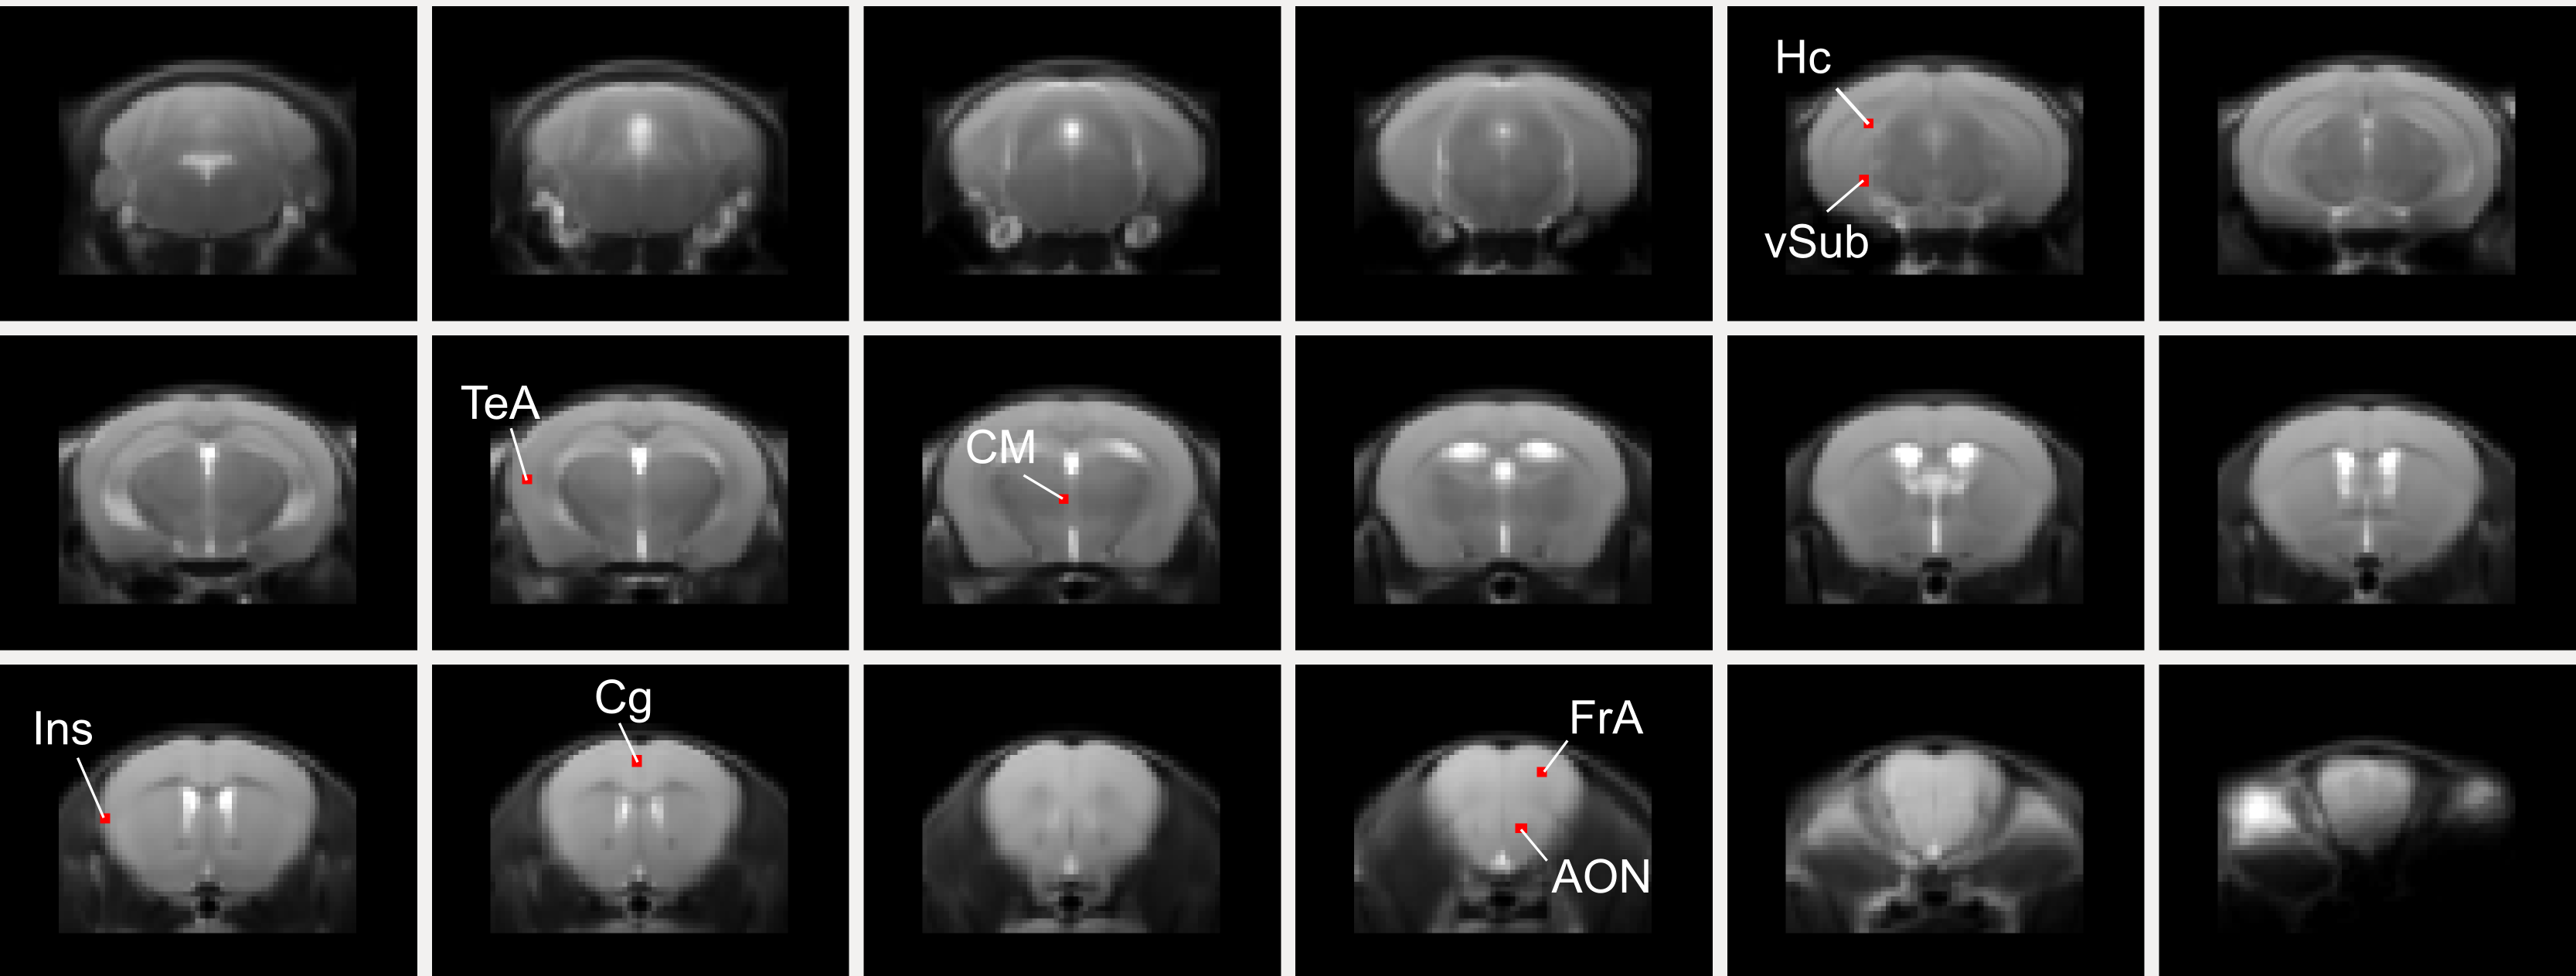
\includegraphics[scale=0.8]{figures/hubs_figure_s1_seed_locations_NEW.png}
    \decoRule
    \caption[Locations seeds used for inter-module hub connectivity
    analysis.]{Locations seeds used for inter-module hub connectivity analysis,
    each displaying the largest value of the network attribute in question for
    the given hub regions, overlaid on the anatomical template. }
    \label{fig:hubs_figs1_seed_location}
\end{figure}

\begin{figure}[th]
    \centering
    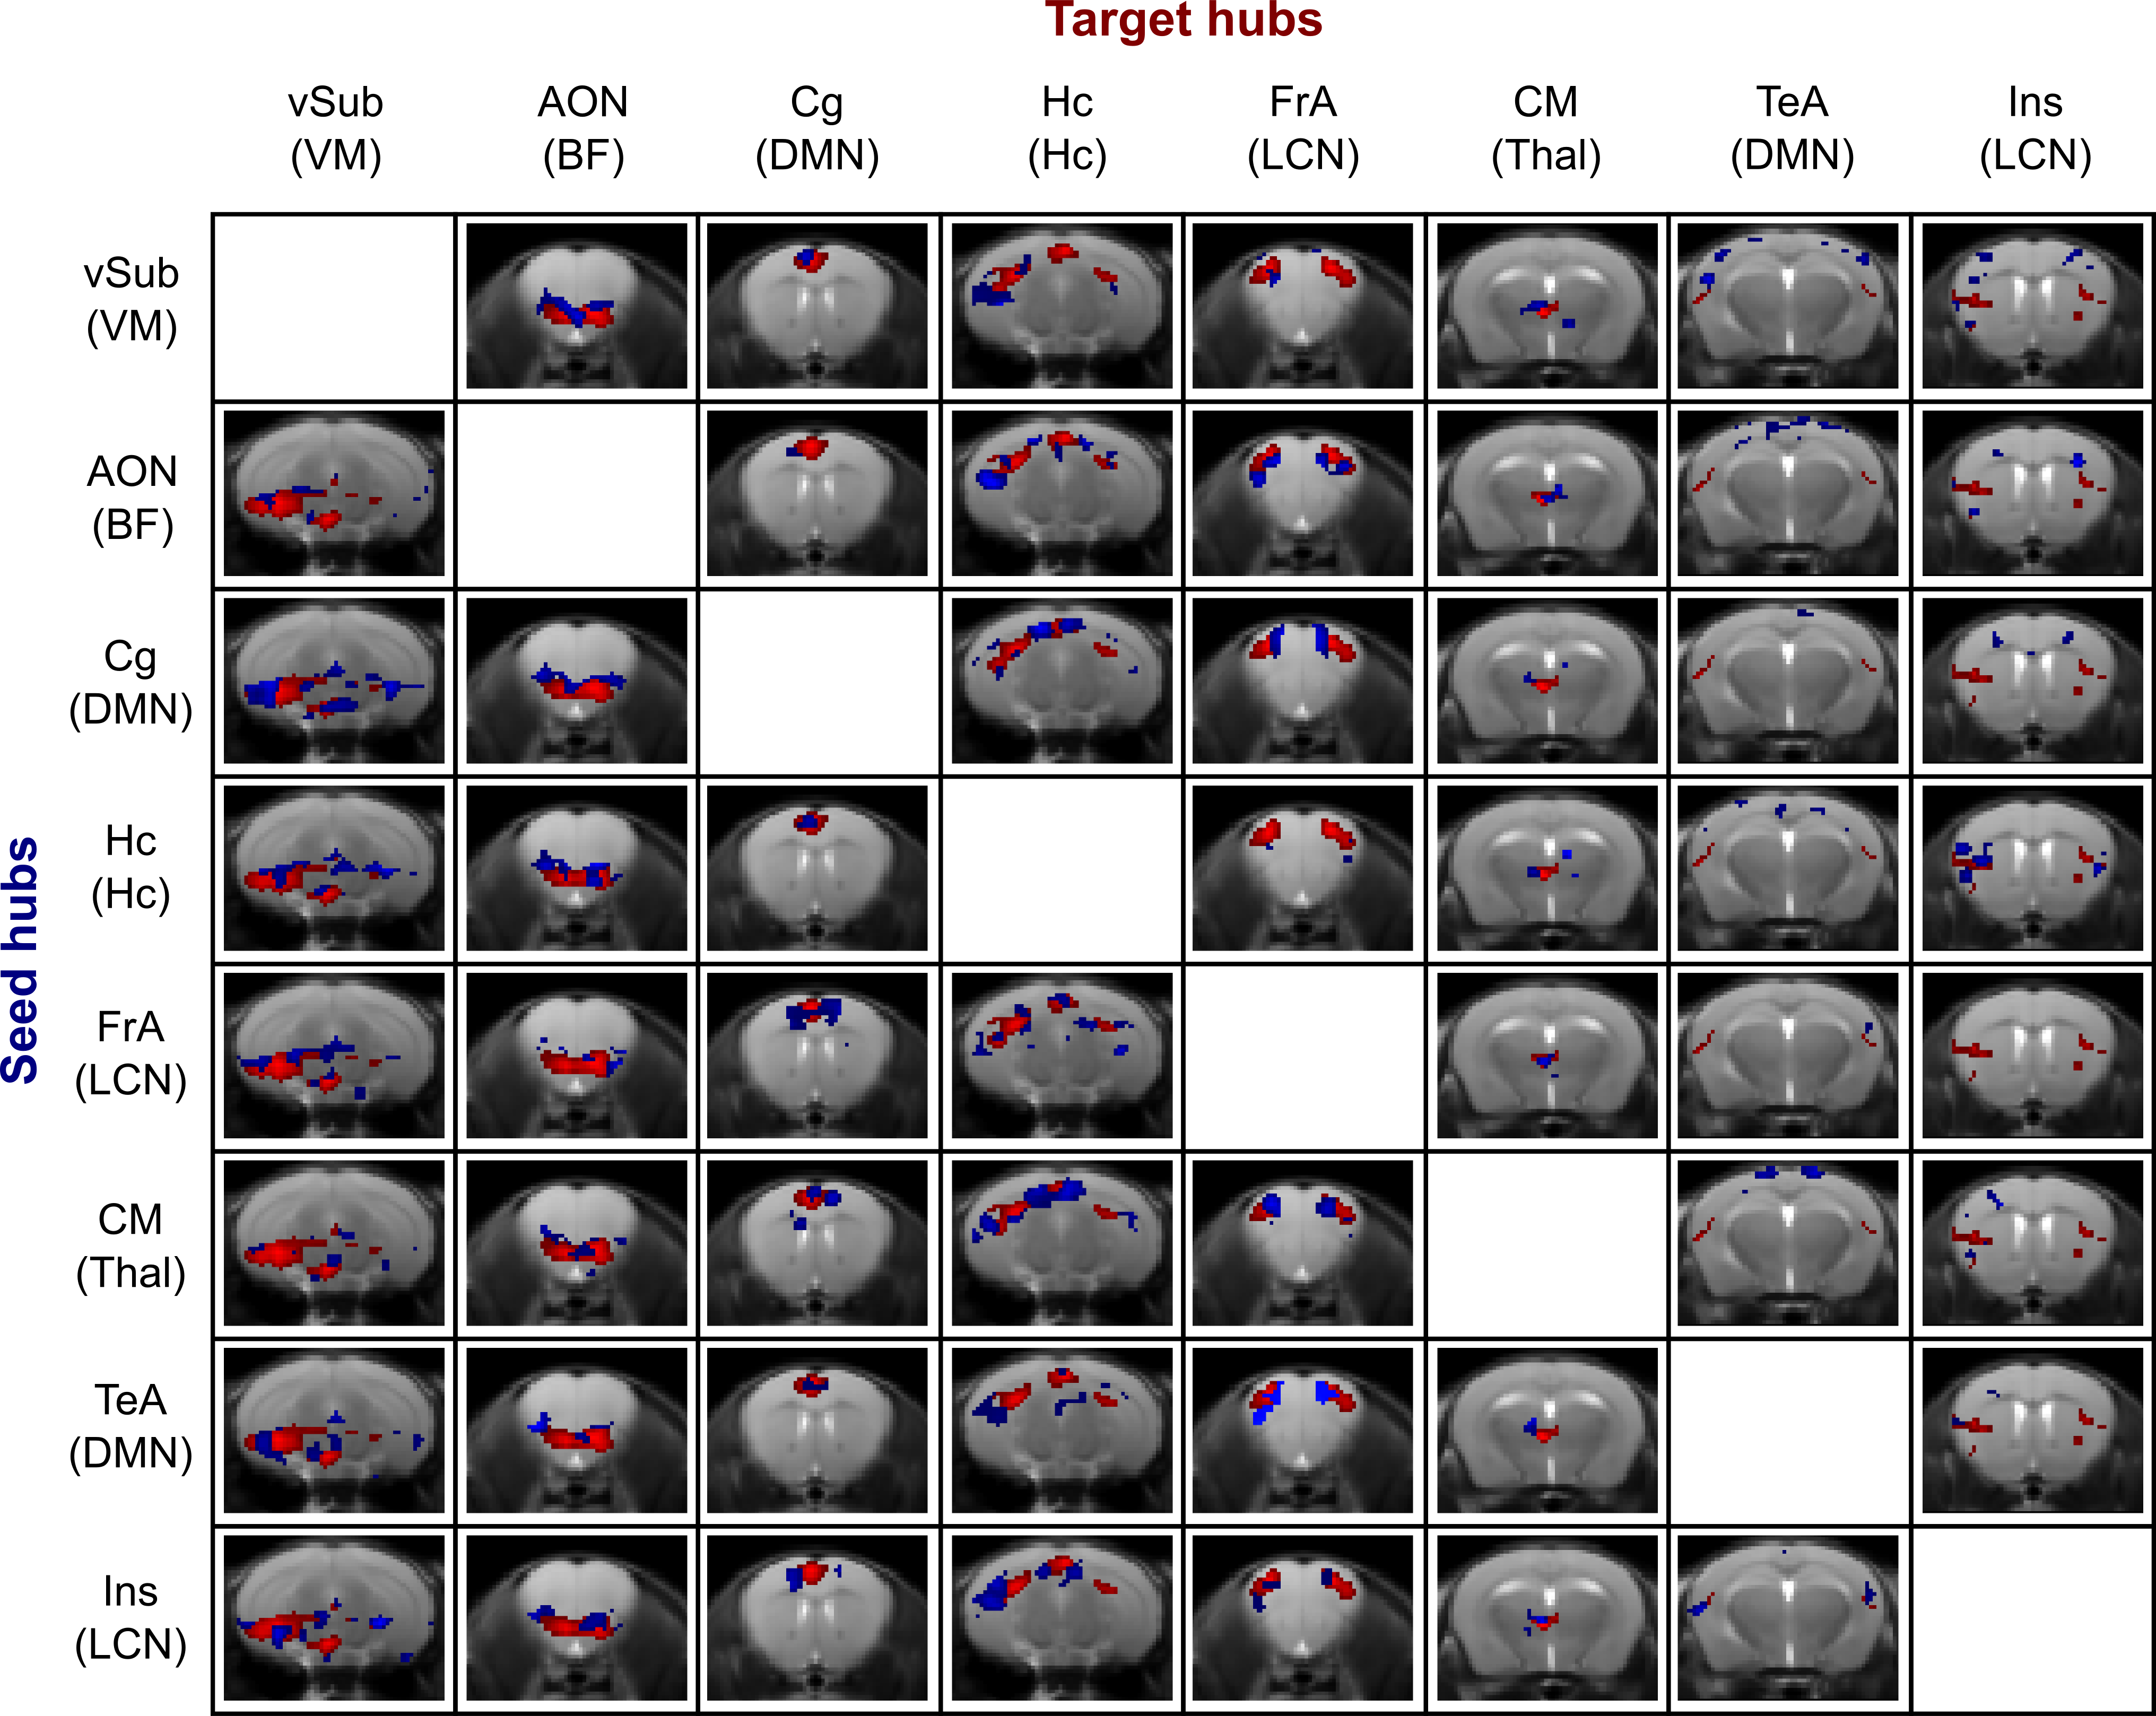
\includegraphics[scale=0.7]{figures/hubs_figure_05_voxel_overlap_NEW.png}
    \decoRule
    \caption[Functional hubs are mutually interlinked.]{Functional hubs are
    mutually interlinked. The strongest connections of each source hub to
    modules of target hubs (thresholded at 90th percentile for each module, in
    blue) are overlaid on top of target hub regions (in red). The results are
    shown on a representative coronal slice for each of the hub-module pair.}
    \label{fig:hubs_fig5_hub_connectivity}
\end{figure}

\begin{figure}[th]
    \centering
    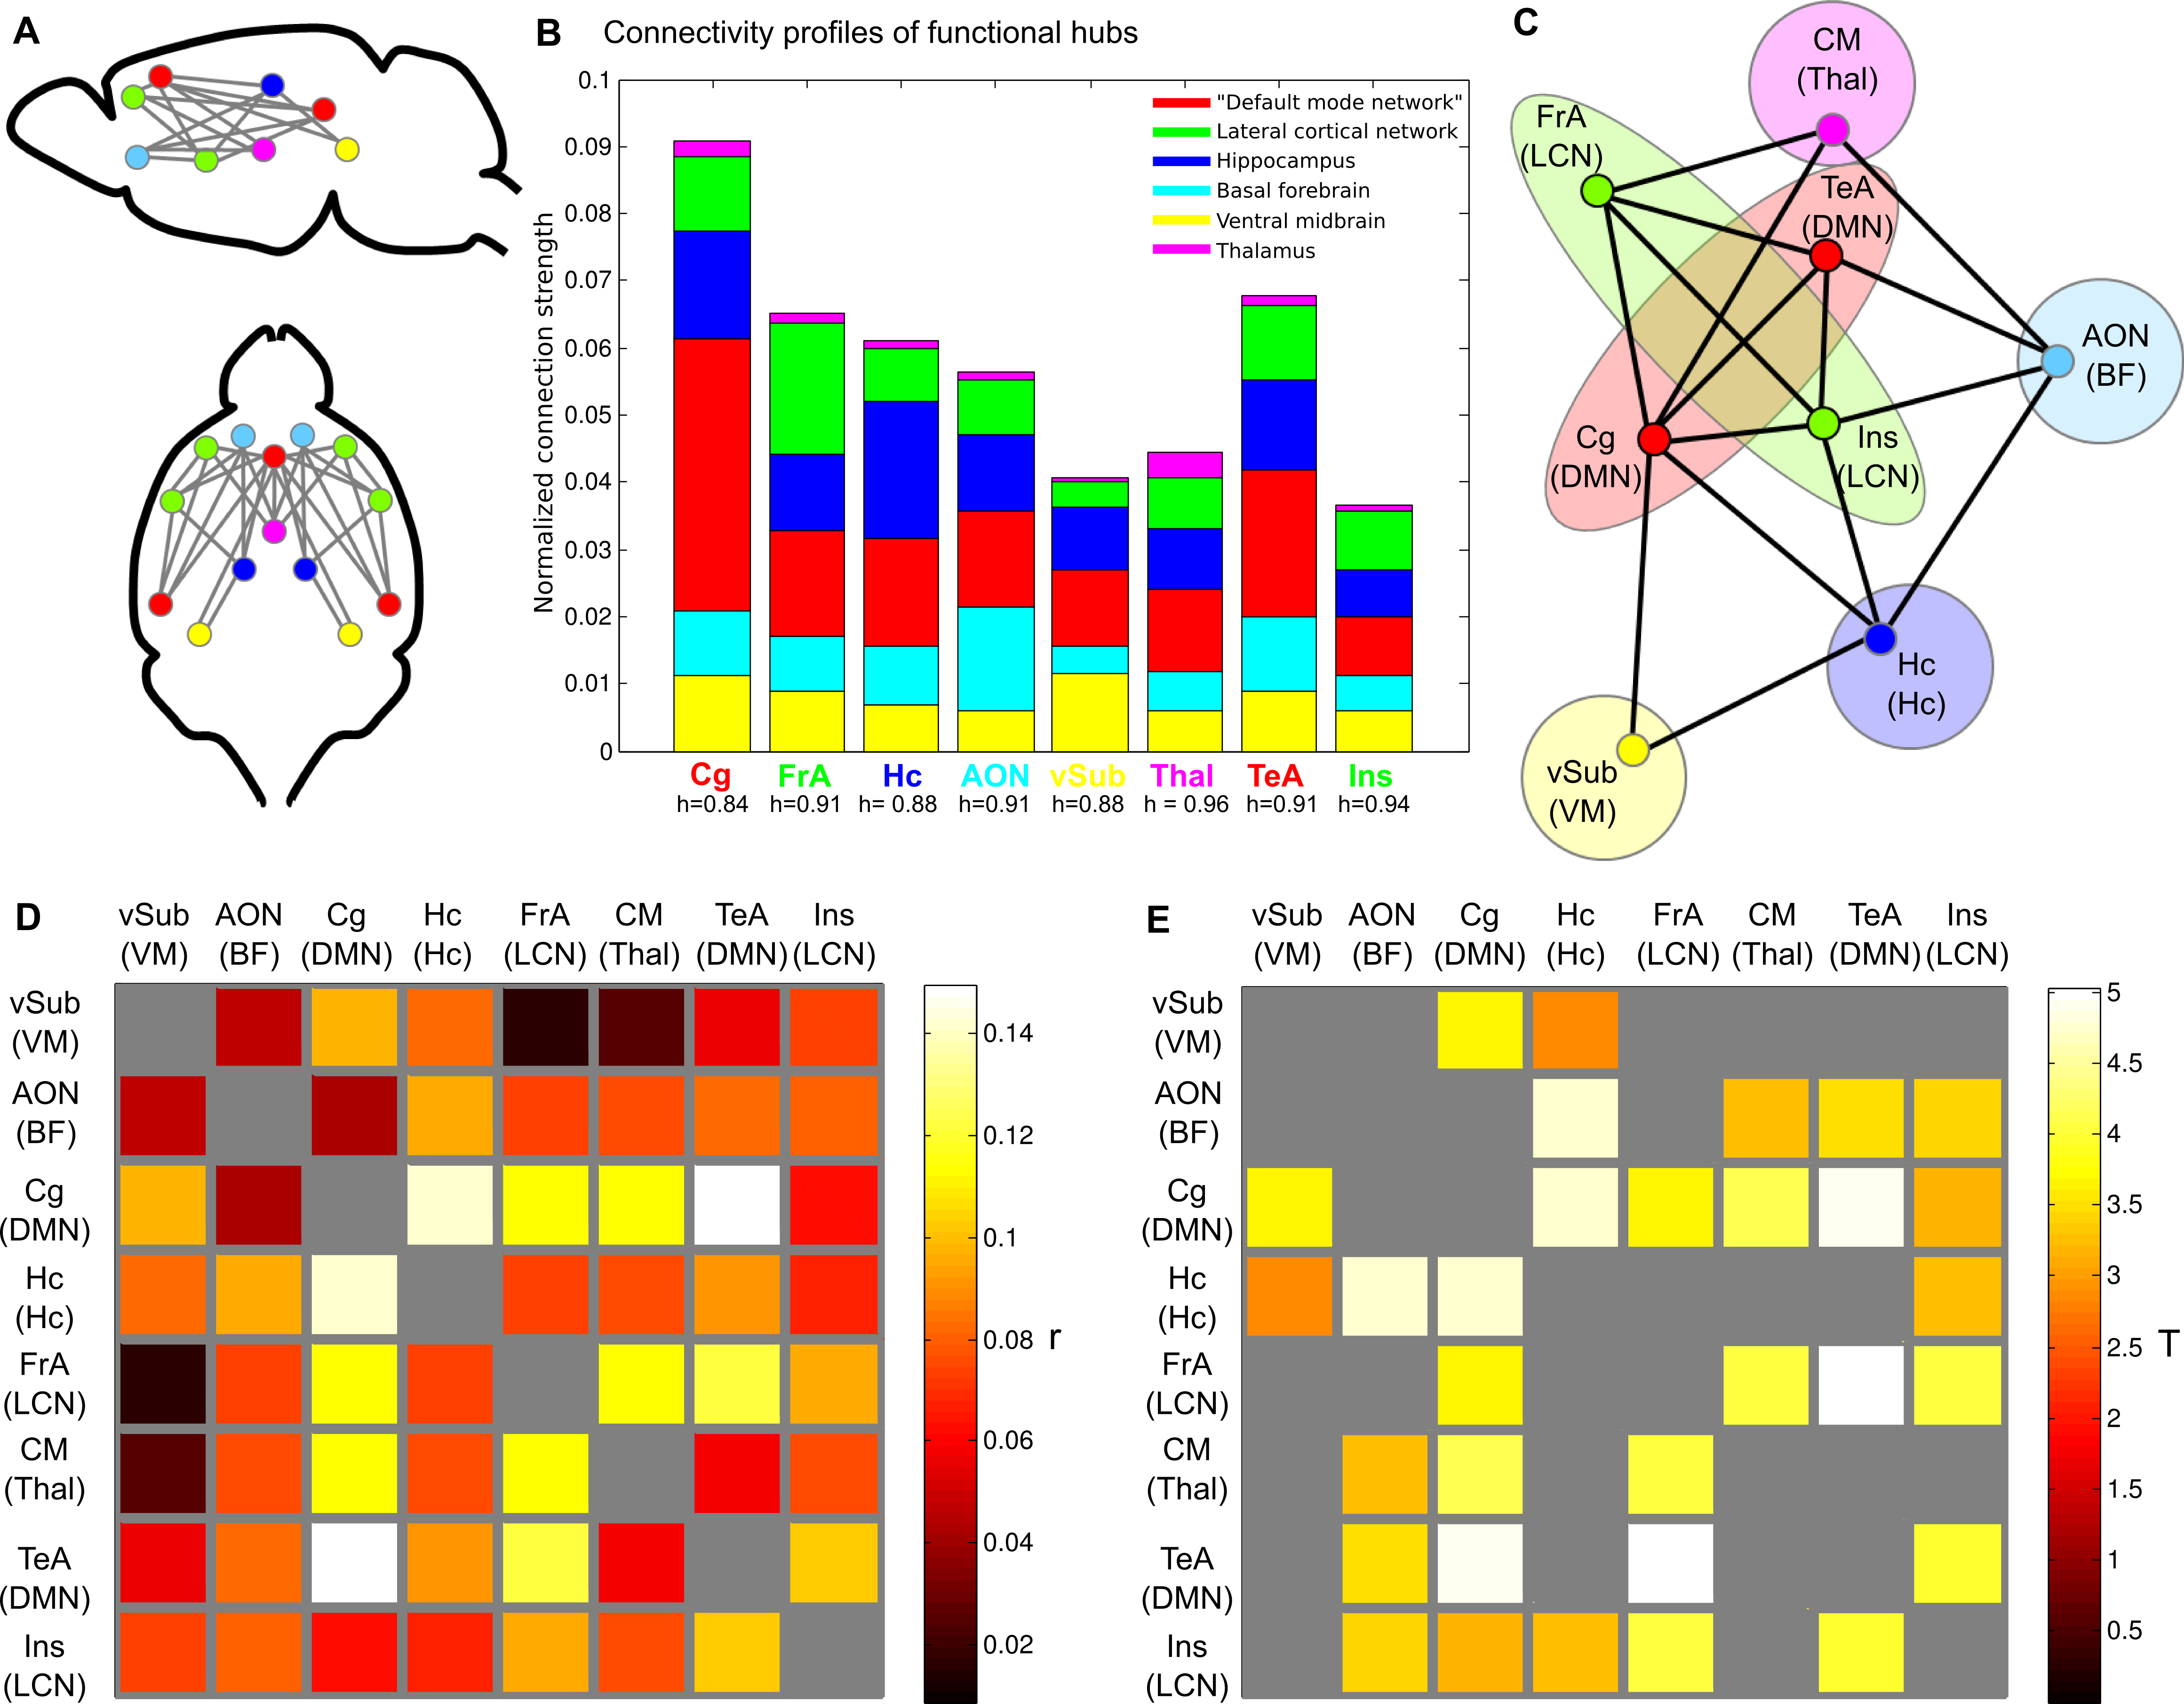
\includegraphics[scale=0.7]{figures/hubs_figure_06_hubs_connections_composite_NEW.png}
    \decoRule
    \caption[Connectivity relationships of candidate hubs.]{(\textbf{A})
    Approximate locations of candidate hubs of the mouse brain. Connections
    surviving statistical thresholding are indicated by a link between nodes
    (\textbf{B}) Connectivity profiles of candidate hubs, showing the proportion
    of their strength across all modules. (\textbf{C}) Graph representation of
    the connections surviving statistical thresholding, with node positions
    determined using the GEM algorithm. (\textbf{D}) Average correlation matrix
    for all pairs of identified hubs. (\textbf{E}) One sample t-tests for all
    pairs of identified hubs; non-significant connections (after FDR correction)
    are shown in grey.}
    \label{fig:hubs_fig6_hub_relationshiops}
\end{figure}


The interconnections between the eight candidate hubs were then characterised
directly to better elucidate the module connectivity that they subserve
(Fig.~\ref{fig:hubs_fig6_hub_relationshiops}). Many, but not all, of the hub
connections were significant, with the cingulate node (DMN module) having the
highest number of significant connections (6) to other candidate hubs, and the
temporal association cortex node (DMN) exhibiting the statistically strongest
connections, namely to the cingulate node (within-module) and to the frontal
association cortex node (across-modules, LCN). The ventral subiculum node (VM
module) had the least number (2) of significant connections to other candidate
hubs, to the cingulate cortex and hippocampal nodes (both across-modules, DMN
and Hc modules respectively).  Notably, both the DMN and LCN modules each
featured two putative cortical hubs, highlighting a key contribution of cortical
hubs within these circuits (i.e.  cingulate, temporal, frontal association, and
insular cortices) as prominent integrative nodes of rsfMRI connectivity networks
in the mouse brain. 

The connectional profiles of candidate hubs attest to the widespread
connectivity of hubs both within their own module and across the whole
functional network (Fig.~\ref{fig:hubs_fig6_hub_relationshiops}B).
Interestingly, a prominent integrative role of the DMN module was apparent, as
this region receives the largest share of the connection strength from all hubs
(excepting connections within a hub’s own module), although it is only second in
size to the ventral midbrain module.

\section{Discussion}

We have demonstrated the presence of distinct functional modules in the mouse
brain, and a set of anatomically localised, mutually interconnected candidate
hub regions acting as cross-module functional integrators. Our approach provides
a fine-grained description of the mouse functional connectome that can serve as
a reference and complement ongoing research in the meso- and large-scale
connectional architecture of this species \parencite{oh2014, stafford2014,
zingg2014}. It
also opens the way to targeted manipulations of hub nodes in mouse models of
brain pathology, a line of research that may advance our understanding of the
elusive role of functional hub regions in neuropsychiatric states
\parencite{vandenheuvel2013}. Importantly, we interrogated the mouse connectome at a
high, voxel-scale spatial resolution and worked with fully-connected,
fully-weighted networks, hence minimising bias induced by parcellation schemes
and issues associated with arbitrary thresholding and/or binarisation
\parencite{bullmore2009}.

Modular organization is central to functional segregation in the brain, whereby
distinct neuronal processing is performed by regions organized in functional
modules \parencite{sporns2013}. Studies of functional modular organization in the human
brain have consistently reported the presence of distinct distributed modules
corresponding to known functional brain systems, such as the default mode,
dorsal attention or somato-motor networks \parencite{meunier2009, power2011,
yeo2011}. In
keeping with this, the mouse brain functional networks identified here can be
reliably related to established large-scale neuro-functional and neuroanatomical
systems of the mammal brain. The detection of a DMN module using graph-based
approaches is in good agreement with the results of classic (ICA- and
seed-based) rsfMRI network mappings in the rodent brain \parencite{schwarz2013a,
schwarz2013, sforazzini2016, stafford2014} and underscores the pivotal role of
this integrative network across mammal brain evolution \parencite{lu2012}. Similarly, the
presence of a lateral cortical module is in agreement with recent
seed-correlation and ICA rsfMRI studies in mice and rats where the presence of a
similar DMN-anticorrelated systems has been described \parencite{schwarz2013a,
schwarz2013, sforazzini2016}, thus leading to the hypothesis that such a network
could be a precursor of lateralised “task-positive” executive modules present in
humans and primates \parencite{fox2005}. Importantly, the identification of
functionally-distinct antero-posterior distributed cortical module components is
in excellent agreement with recent cortical connectivity mapping obtained with
tracer injections in the mouse cortex. Indeed, by applying graph-based analyses
of tracer-based structural connectivity, \textcite{zingg2014} identified two
major neocortical clusters (i.e., somatic sensorimotor and medial
antero-posterior networks) that exhibit remarkable  neuroanatomical overlap
with our LCN and DMN modules. Similarly, the same authors also identified two
lateral integrative subnetworks in the cortex (anterior insular and posterior
temporal) that can be related to the high connection diversity cortical hub
nodes identified in the present work. Collectively, these findings corroborate
the emerging view that functional correlations in spontaneous brain activity
are constrained and guided by patterns of anatomical connectivity
\parencite{honey2009, sui2014}, a notion that has been more recently
demonstrated also for the mouse brain \parencite{stafford2014}. 

The correspondence between our cortical modules and analogous functional
networks of the human brain is of high translational relevance, as the approach
permits to identify key topological landmarks that can guide cross-species
extrapolation of neural circuit research in health and pathology. In this
respect, our work represents a significant advance over previous graph-based
attempts to unravel the rodent’s functional topology \parencite{bifone2010,
dsouza2014, liang2011, liang2012, schwarz2008, schwarz2009}. Indeed, while these
previous studies identified plausible functional modules, including large
cortical partitions \parencite{liang2011} and some subcortical networks similar
to those described here (e.g.  basal ganglia and hippocampus)
\parencite{dsouza2014, liang2011}, they did not to reveal antero-posterior
cortical networks like the rat’s DMN module, or the lateral cortical system, a
finding that could reflect discrepant experimental procedures as well as
heterogeneity in the regional parcellation schemes (coarse ICA-based or
anatomical volumes) and network thresholding strategies employed, or the fact
that the initial graph-based parcellation used cross-subject analyses of
responses to pharmacological stimuli \parencite{bifone2010, schwarz2008,
schwarz2009}. Likewise, the results of a recent attempt to map functional
modules and hubs in the mouse employing ICA-based functional parcellation
\parencite{mechling2014} resulted in a coarse modular organization that includes
some of the modules identified in this study (e.g. basal ganglia and
hippocampus), as well as a combination of cortical and subcortical structures
encompassing multiple neurofunctional systems of the brain (e.g. sensory motor
and limbic areas), which corroborate the underlying modular structure of the
mouse brain, but cannot be directly related to analogous functional modules of
the human brain.  The identification of neuro-biologically interpretable
functional modules is also key to the identification of candidate hub regions
deemed to link and integrate specialized functional systems
\parencite{sporns2013}. Using graph-based methods, numerous studies in humans
have converged on a limited set of regions that occupy a central position in the
functional topology of the human brain. These regions include anterior and
posterior cingulate cortices, the insular cortex, and portions of superior
frontal cortex, temporal cortex and lateral parietal cortex \parencite{cole2010,
sporns2014, tomasi2011, vandenheuvel2013}. Importantly, the very same regions
have also been shown to be implicated in the anatomy of various brain disorders,
such as schizophrenia and Alzheimer’s disease, which can be investigated and
modelled in the mouse \parencite{buckner2009, crossley2014}. Consistent with
human findings \parencite{cole2010}, we identified high strength nodes in the
mouse brain located in midline regions within the DMN module, with a predominant
involvement of integrative areas such as the prefrontal, anterior and posterior
cingulate cortex. Notably, a striking neuroanatomical correspondence also exists
between our high connection strength hubs, and high degree structural
connectivity hubs of the mouse based axonal tracing \parencite{stafford2014}, a
finding that recapitulates a fundamental neuro-architectural feature of the
human brain \parencite{vandenheuvel2013}. Similarly, high connection
diversity regions were identified in the temporal association cortex and, albeit
with a lower degree of statistical confidence, also in the anterior insula, two
areas classically implicated in multimodal integration \parencite{gogolla2014}.
Furthermore, the same areas have been recently described in the human brain as
regions of high participation coefficient, a binary network counterpart to
connection diversity \parencite{power2013}. Importantly, most of the hub regions
we identified in the mouse brain exhibit robust and specific mutual
inter-connections, a finding which is consistent with an integrative functional
role of these nodes, and which argues against a predominant confounding
contribution of the correlational nature of rsfMRI-based networks
\parencite{power2013}.  Collectively, these correspondences underscore the
translational relevance of our findings, and support the notion that the mouse
brain contains evolutionary-conserved cortical foci serving as integrators of
segregated systems in the mammal brain.

The fact that our experiments were performed in anaesthetized animals raises the
question as to the degree to which the observed effects reflect the functional
architecture of the mouse brain in conscious states. Two recent mouse rsfMRI
studies have highlighted different connectivity signatures and reduced
inter-hemispheric connectivity as a function of anaesthetic regimen
\parencite{grandjean2014, jonckers2014}. The present work was performed in
halothane-anaesthetised animals, a regimen that appears to be particularly
suited to map distributed rsfMRI circuits in this species for several reasons.
First, halothane ensures motion control and stable hypnosis while preserving
cerebral blood flow autoregulation \parencite{gozzi2007} and cortical electrical
responsiveness \parencite{orth2006} without the occurrence of burst suppression
activity, a phenomenon associated with significant rsFC alterations
\parencite{liu2011}.
Consistent with this, our recent work \parencite{sforazzini2014, sforazzini2016,
zhan2014} demonstrates the presence of (1) robust homotopic inter-hemispheric
functional connectivity in both cortical and subcortical areas, and (2)
distributed networks remarkably similar to those seen in conscious (and lightly
anesthetised) rats and primates, anatomically homologous to the human salience
network (SN) and default-mode network (DMN) \parencite{hutchison2010, lu2012,
rilling2007, schwarz2013, schwarz2012, vincent2007}. Importantly, the
observation of a DMN-like network in the mouse has been recently replicated by
an independent group \parencite{stafford2014} using a different anaesthetic
(isoflurane), a finding that corroborates a neurobiological foundations of this
cortical module. Moreover, BOLD fMRI oscillations in the DMN-like network
exhibit anti-correlations with neighbouring fronto-parietal areas, a cardinal
feature of the human and primate DMN \parencite{fox2005}. By showing analogous
networks using cerebral blood volume weighted signals, we also demonstrated that
these spontaneous fluctuations are not significantly contaminated by large blood
vessels \parencite{sforazzini2016}. Finally, we recently demonstrated excellent
spatial correspondence between rsfMRI signals obtained during light anaesthesia
and electrophysiological coherence signals in freely-behaving animals,
suggesting that the anaesthetic protocol negligibly influences intrinsic rsfMRI
connectivity profiles \parencite{zhan2014}. Collectively, the identified rsfMRI
networks exhibit significant correspondence with analogous measurements in awake
habituated rats and human studies, thus legitimating the extrapolation of our
results to conscious states. Consistent with this notion, global topological
features of rsfMRI networks were found to be well maintained in the anesthetized
rat brain when compared to awake (restrained) states, despite the use of much
higher (2.25-fold) minimal alveolar concentration levels of anaesthetic than the
present work \parencite{eger2003, liang2012, sonner2000}. The remarkable overlap
between modules and hubs identified in this work and recent tract tracing
mapping in the mouse \parencite{zingg2014}, as well as analogous graph-based
mappings in conscious human brain provide further empirical support to a
marginal confounding contribution of anaesthesia to our findings.  

\section{Conclusion}

In conclusion, our results describe topologically distinct neuro-functional
modules of the mouse brain, including a DMN-like module, and identify a set of
mutually-interconnected functional hubs that include well-characterised
integrative cortical structures. These findings reveal the presence of
evolutionarily conserved functional modules and integrative hubs in the mouse
brain, and support the use of this species to investigate the elusive
neurobiological underpinnings of the functional hub aberrations described for
several pathological states. Importantly, our approach also provides a
fine-grained description of the mouse functional connectome that complements and
integrates ongoing research in the large-scale connectional architecture of this
species. 

\chapter{Reduced connectivity in \textit{Cntnap2}-null mice}

\label{Chapter03}

\begin{quote}
    This chapter has been published as:

    \longfullcite{liska2017}
\end{quote}

\section{Background}

Neuroimaging and post-mortem studies have consistently revealed impaired or
atypical connectivity across brain regions of autistic spectrum disorders (ASD)
patients \parencite{anagnostou2011}. These findings have led to the hypothesis
that aberrant connectivity patterns might represent a common final pathway or
neurobiological pathogenetic correlate of the autistic phenotype to which
different ASD etiologies may converge \parencite{just2012}. Although great
heterogeneity exists in the sign and distribution of abnormal connectivity
across studies and imaging modalities, consistent features indeed appear to
emerge, including reduced functional coherence of long-range intra-hemispheric
cortico-cortical default mode circuitry, impaired inter-hemispheric regulation
and possible increase in local and short-range cortico-subcortical coherence
\parencite{rane2015}.  However, the neurophysiological underpinnings of these connectional
derangements are largely unknown, and a causal etiopathological contribution of
specific genetic variants to impaired connectivity in ASD remains to be firmly
established. 

Mouse lines recapitulating high-confidence ASD mutations \parencite{sanders2015}
have been employed to understand how specific genetic alterations translate into
relevant changes in cells and circuits \parencite{auerbach2011}. The recent
optimization of neuroimaging readouts of functional connectivity such as
resting-state functional MRI (rsfMRI) in the mouse \parencite{sforazzini2014}
permits to extend this paradigm to the investigation of the elusive genetic and
neurobiological foundations of aberrant connectivity observed in ASD
\parencite{liska2016}. The approach leverages on the identification of robust
homotopic and distributed rsfMRI connectivity networks in the mouse, including
possible homologues of distributed human rsfMRI systems like the salience and
default mode (DMN) networks \parencite{gozzi2016}, and the observation that
cyto-architecturally conserved heteromodal cortices in cingulate and
retrosplenial regions exhibit similar “hub-like” topological properties in both
species \parencite{cole2010, liska2015}. Importantly, as mouse rsfMRI
measurements rest on the same biophysical principles as corresponding human
neuroimaging readouts, this approach has the merit of providing a direct
translational bridge across species. 

Homozygous loss-of-function mutations in Contactin Associated Protein-like 2
(CNTNAP2) encoding CASPR2, a neurexin-related cell-adhesion molecule, are
strongly linked to autism and epilepsy in consanguineous families
\parencite{strauss2006, alarcon2008, rodenas-cuadrado2014}. Loss of \textit{Cntnap2} in
mice leads to abnormal neuronal migration, reduced GABAergic neurons,
spontaneous seizures, and behavioural traits consistent with ASD symptoms in
humans \parencite{penagarikano2011}, an ensemble of traits that phenocopy major
neuropathological features observed in cortical dysplasia-focal epilepsy (CDFE)
syndrome, a rare neuronal migration disorder associated with a recessive
mutation in CNTNAP2 \parencite{strauss2006}.  Interestingly, common genetic
variants in CNTNAP2 were recently described to be associated with impaired
frontal lobe connectivity in humans \parencite{scott-vanzeeland2010}.  However,
a causal relationship between ASD-related loss-of-function mutations in CNTNAP2
and functional connectivity remains to be firmly established. Moreover, the role
of CNTNAP2 in shaping macroscale circuit assembly, and the specific substrates
affected, remain largely unknown.

To address these questions, we used BOLD rsfMRI, diffusion-weighted MRI and
retrograde viral tracing to map large-scale functional connectivity and white
matter topology in homozygous \textit{Cntnap2}-null mice (\textit{Cntnap2}$^{-/-}$). We document that
loss of \textit{Cntnap2} results in local and long-range connectivity reductions
affecting prefrontal regions that act as “functional connectivity hubs” in the
mouse brain \parencite{liska2015}, and that fronto-posterior hypo-connectivity
is associated with impaired social behaviour. The presence reduced
prefrontal-projecting neuronal frequency in the cingulate cortex of \textit{Cntnap2}$^{-/-}$
mutants suggest a possible contribution of defective mesoscale axonal wiring to
the observed functional connectivity impairments. Collectively, these results
reveal a role of autism-risk gene CNTNAP2 in modulating functional network
assembly between key integrative connectivity hubs of the mammalian brain. The
observed long-range prefrontal hypo-connectivity in \textit{Cntnap2}$^{-/-}$ mice
recapitulates imaging findings in autism and adds to the construct validity of
this mouse line to model ASD-related phenotypes.

\section{Materials and methods}

\subsection {Ethical statement}

All in vivo studies were conducted in accordance with the Italian law (DL 116,
1992 Ministero della Sanità, Roma) and the recommendations in the Guide for the
Care and Use of Laboratory Animals of the National Institutes of Health. Animal
research protocols were also reviewed and consented to by the animal care
committee of the Istituto Italiano di Tecnologia. The Italian Ministry of Health
specifically approved the protocol of this study, authorization no. 07753 to A.G.
All surgical procedures were performed under anaesthesia.

\subsection{Animals}

\textit{Cntnap2}-null (\textit{Cntnap2}$^{-/-}$) and control “wild-type” (\textit{Cntnap2}$^{+/+}$) breeding pairs
were obtained from Jackson Laboratories (Bar Harbor, ME, USA) and bred locally.
Mice were housed by sex in mixed genotype groups, with temperature maintained at
$21 \pm 1\degree C$ and humidity at $60 \pm 10 \%$. All experiments were
performed on adult male mice between 12-16 week of age, corresponding to young
maturity. The specific age-range for each experimental activity is reported
below. No onset of spontaneous seizures was observed in any of the \textit{Cntnap2}
mutants or control mice tested in behavioural, imaging or tracing studies. This
is consistent with previous reports showing propensity for spontaneous epileptic
episodes in \textit{Cntnap2}$^{-/-}$to occur only after 6 months of age
\parencite{penagarikano2011}.

\subsection{Social interaction}

For behavioural testing, 12-week-old \textit{Cntnap2}$^{-/-}$ and control \textit{Cntnap2}$^{+/+}$ mice (n =
13 each group), were evaluated in the male–female social interaction test during
the light phase, as previously described \parencite{scattoni2011, scattoni2013}.
An unfamiliar stimulus control female mouse in estrous was placed into the
home-cage of an isolated test male mouse, and social behaviour were recorded
during a 3-min test session. Scoring of social investigation parameters was
conducted using Noldus Observer 10XT software (Noldus Information Technology,
Leesburg, VA, USA). Social interactions were defined as number of events
(frequency) and duration of the following behavioural responses performed by the
test mouse: anogenital sniffing (direct contact with the anogenital area), body
sniffing (sniffing or snout contact with the flank area), head sniffing
(sniffing or snout contact with the head/neck/mouth area), locomotor activity,
rearing up against the wall of the home-cage, digging in the bedding, and
grooming (self-cleaning, licking any part of its own body). Social investigation
is defined as the sum of sniffing and following behaviours
\parencite{scattoni2008}. No observations of mounting, fighting, tail rattling,
and wrestling behaviours were observed. Scoring was rated by two investigators
blind to genotype. Inter-rater reliability was 98 \%. To measure ultrasound
vocalization recordings, an ultrasonic microphone (Avisoft UltraSoundGate
condenser microphone capsule CM16, Avisoft Bioacoustics, Berlin, Germany) was
mounted 20 cm above the cage and the USVs recorded using Avisoft RECORDER
software version 3.2. Settings included sampling rate at 250 kHz; format 16 bit.
The ultrasonic microphone was sensitive to frequencies between 10 and 180 kHz.
For acoustical analysis, recordings were transferred to Avisoft SASLabPro
(version 4.40) and a fast Fourier transformation (FFT) was conducted as
previously described \parencite{scattoni2008}. Start times for the video and
audio files were synchronized. 

\subsection{Resting-state fMRI}

rsfMRI experiments were performed on the same experimental cohorts employed in
the behavioural tests ($n = 13$ \textit{\textit{Cntnap2}}$^{+/+}$; $n = 13$ \textit{\textit{Cntnap2}}$^{-/-}$). At the time of
imaging, mice were 13-14 weeks old. The animal preparation protocol was recently
described in great detail \parencite{ferrari2012, sforazzini2016}. Briefly, mice
were anaesthetized with isoflurane (5 \% induction), intubated and artificially
ventilated (2 \% maintenance). The left femoral artery was cannulated for
continuous blood pressure monitoring and terminal arterial blood sampling. At
the end of surgery, isoflurane was discontinued and substituted with halothane
(0.75 \%). Functional data acquisition commenced 45 min after isoflurane
cessation. Mean arterial blood pressure was recorded throughout imaging
sessions. Arterial blood gases (paCO2 and paO2) were measured at the end of the
functional time series to exclude non-physiological conditions. Mean paCO2 and
paO2 levels recorded were $17 \pm 3$ and $250 \pm 29$ mmHg in \textit{\textit{Cntnap2}}$^{+/+}$ and $15
\pm 3$ and $231 \pm 38$ mmHg in \textit{\textit{Cntnap2}}$^{-/-}$. Possible genotype-dependent
differences in anaesthesia sensitivity were evaluated using Student’s two-sample
t-test applied to two independent readouts previously shown to be linearly
correlated with anaesthesia depth: mean arterial blood pressure and amplitude of
cortical BOLD signal fluctuations \parencite{steffey2003, liu2011, zhan2014}.

rsfMRI images were acquired with a 7.0 Tesla MRI scanner (Bruker Biospin, Milan)
as previously described \parencite{liska2015}, using a 72 mm birdcage transmit
coil and a four-channel solenoid coil for signal reception. For each session,
high-resolution anatomical images were acquired with a fast spin echo sequence
(repetition time (TR)/echo time (TE) 5500/60 ms, matrix $192 \times 192$, field
of view $2 \times 2 \text{cm}^2$, 24 coronal slices, slice thickness 0.50 mm).
Co-centred single-shot BOLD rsfMRI time series were acquired using an echo
planar imaging sequence with the following parameters: TR/TE 1200/15 ms, flip
angle $30\degree$, matrix $100 \times 100$, field of view $2 \times 2 \text{cm}^2$, 24
coronal slices, slice thickness 0.50 mm, 500 volumes and a total rsfMRI
acquisition time of 10 min. Readers can contact the corresponding author for
access to the MRI raw data, templates and code employed to generate the
functional maps.

\subsection{Functional connectivity analyses}

The first 20 volumes of the rsfMRI data were removed to allow for T1
equilibration effects. The time series were then despiked, corrected for motion
and spatially normalized to an in-house mouse brain template
\parencite{sforazzini2014}.  The normalised data had a spatial resolution of
$0.1042 \times 0.1042 \times 0.5$ mm$^3$ ($192 \times 192 \times 24$ matrix).
Head motion traces and mean ventricular signal (averaged rsfMRI time course
within a reference ventricular mask) were regressed out of each of the time
series. No inter-group differences in ventricular volume was observed as
measured by the dimension of individual ventricular masks (t-test, p = 0.31).
All rsfMRI time series were spatially smoothed (full width at half maximum of
0.6 mm) and band-pass filtered to a frequency window of 0.01-0.1 Hz. 

To obtain an unbiased identification of the brain regions exhibiting
genotype-dependent differences in functional connectivity, we implemented
recently developed aggregative metrics for these parameters \parencite{cole2010,
maximo2013, liska2015} and calculated local and global connectivity maps for all
subjects. This metric considers connectivity of a given voxel to a subset of all
other voxels within the brain mask by computing average connectivity strength.
Specifically, we employed the weighted connectivity method, in which individual
r-scores are first transformed to z-scores using Fisher’s r-to-z transform and
then averaged to yield the final connectivity score. Local connectivity strength
was mapped by limiting this measurement to connections within a 6-voxel radius
sphere (0.6252 mm in plane), while long-range connectivity was computed by
considering only connections to voxels outside this sphere. The radius employed
represents approximately half the thickness of mouse anterior cortex
\parencite{dodero2013} and is a good approximation of the overall average
cortical thickness \parencite{braitenberg1998, sun2014}. The use of this value
ensures that the employed local connectivity metric reflects purely
intra-cortical effects at least in outmost cortical voxels and in thicker
fronto-cortical regions. This value is proportionally much lower than what is
commonly employed in human local connectivity mappings, where values as large as
14 mm (i.e., 4/5-fold mean human cortical thickness) have been employed
[reviewed by \parencite{maximo2013}].

Voxelwise inter-group differences in each of these parameters were mapped using
a two-tailed Student’s t-test (p < 0.05 FWE cluster corrected with
cluster-defining threshold of t24 > 2.06, p < 0.05, as implemented in FSL). The
effect was also quantified in volumes of interest (VOIs). The anatomical
location of the examined VOIs is reported in Fig.~\ref{fig:cntnap2_figs1}.
Region identification and naming follow classic neuroanatomical labelling
described in \parencite{paxinos2004}.  Many of these regions have recently been
reclassified according to their cytoarchitectural properties such to match
analogous regions in human and primates \parencite{vogt2014}. According to this
scheme, the mouse prelimbic cortex corresponds to Brodmann area 32 (A32),
cingulate cortex area 1 (anterior cingulate cortex) to Brodmann area A24b,
infralimbic cortex to A24a, retrosplenial cortex to areas A30 and A29. In
keeping with this and the comparative work of other authors
\parencite{ongur2000}, in this paper we define the mouse prefrontal cortex (PFC)
as an anatomical ensable of regions inluding prelimbic, infralimbic and anterior
cingulate cortex, corresponding to Brodmann areas A24a/b, A32, and A10.

\begin{figure}[th] 
    \centering
    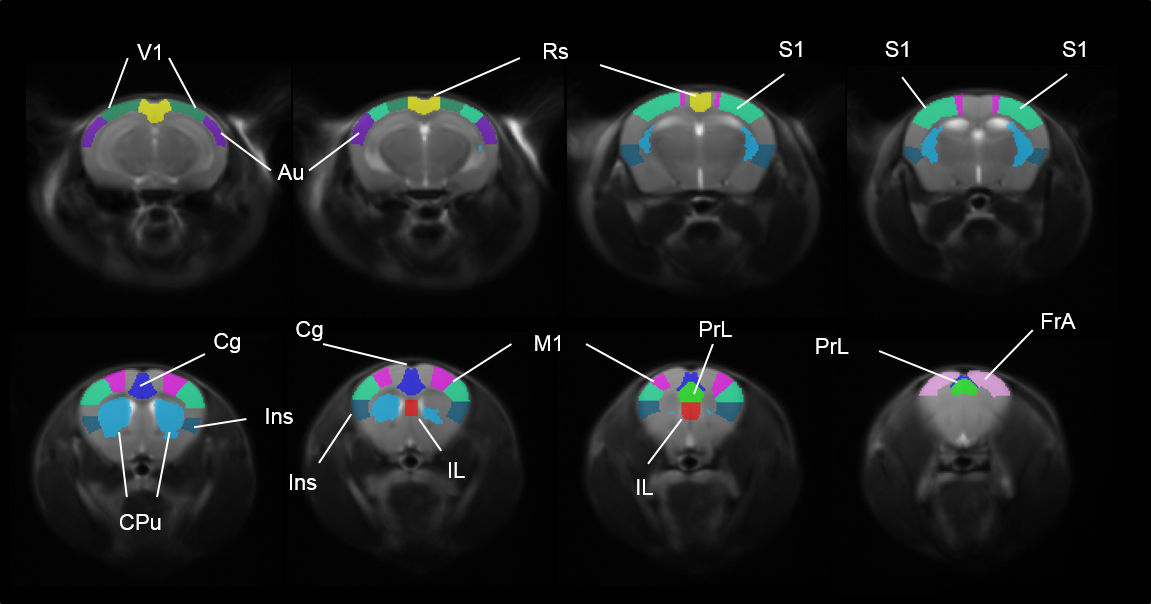
\includegraphics[scale=0.6]{figures/cntnap2_figure_s1.png}
    \decoRule
    \caption[Volumes of interest used in functional connectivity mappings.]{V1,
    primary visual cortex; Au, auditory cortex; Rs, retrosplenial cortex; S1,
    primary somatosensory cortex; Cg, cingulate cortex; CPu, caudate-putamen;
    Ins, insular cortex; IL, infra-limbic cortex; M1, primary motor cortex; PrL,
    prelimbic cortex; FrA, frontal association cortex.}
    \label{fig:cntnap2_figs1}
\end{figure}

Inter-group differences in the extension and intensity of long-range rsfMRI
correlation networks were mapped using seed-based approach as previously
described \parencite{sforazzini2016}. Small a priori seed regions of $3 \times 3
\times 1$ voxels were chosen to cover antero-posterior cortical networks and
representative heteromodal cortical structures (Fig.~\ref{fig:cntnap2_figs2}).
The mean time courses from the unilateral (medial, Rs, PrL) and bilateral seeds
(TeA, Pt, and vHC) were used as regressors for each voxel. Group level
differences in connectivity distributions were mapped using two-tailed Student’s
t-tests (p < 0.05 FWE cluster corrected with cluster-defining threshold of t24 >
2.06, p < 0.05, as implemented in FSL).

\begin{figure}[th] 
    \centering
    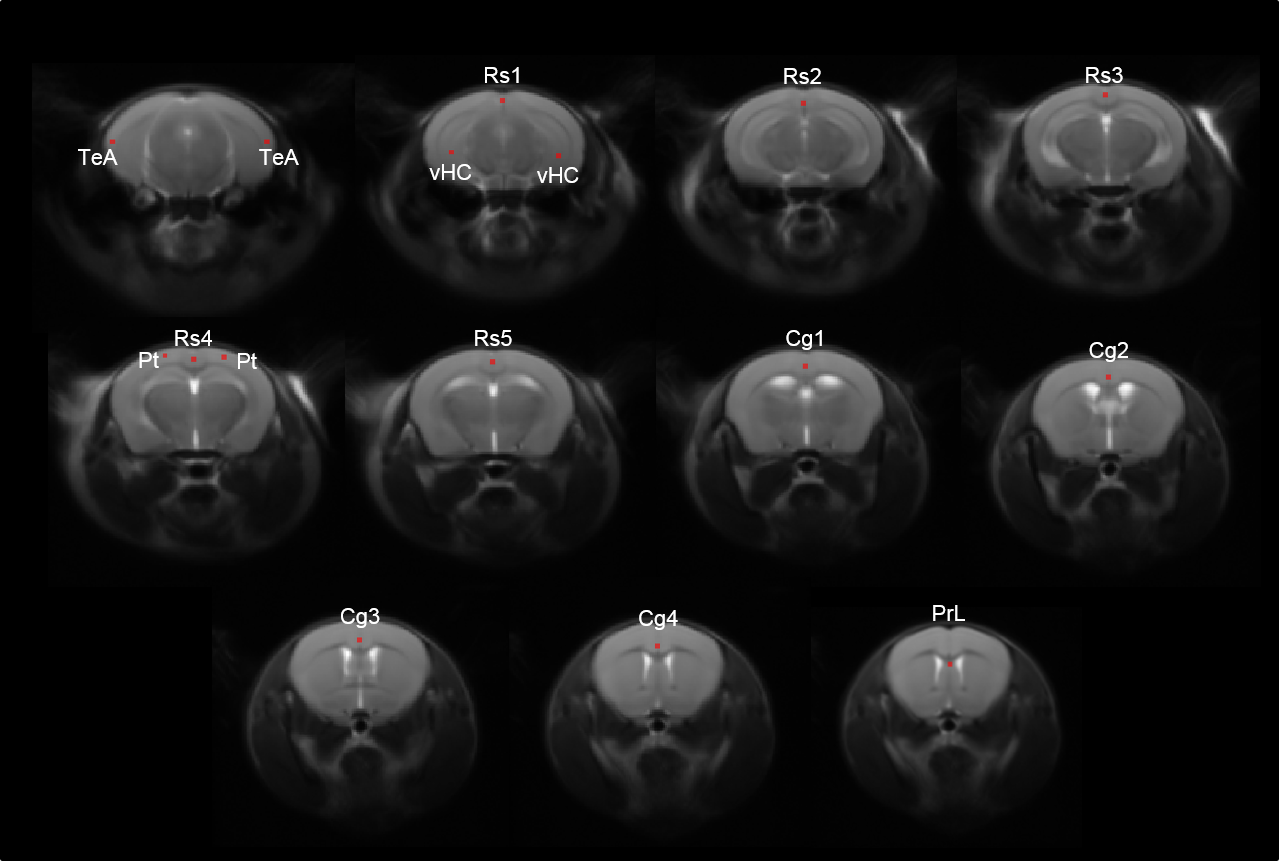
\includegraphics[scale=0.6]{figures/cntnap2_figure_s2.png}
    \decoRule
    \caption[Location of seeds used in mapping anteroposterior DMN
    connectivity.]{Location of seeds used in mapping anteroposterior DMN
    connectivity. TeA, temporal association cortex (bilateral); Rs,
    retrosplenial cortex; Cg, cingulate cortex; Pt, posterior parietal
    association cortex (bilateral); PrL, prelimbic cortex; vHC: ventral
    hippocampus.}
    \label{fig:cntnap2_figs2}
\end{figure}

Alterations in inter-hemispheric functional connectivity were assessed by
computing correlation coefficients of inter-hemispheric VOI pairs depicted in
Fig.~\ref{fig:cntnap2_figs1}. The statistical significance of inter-group
correlation strength in each VOI was assessed with a two-tailed Student’s t-test
(t24 > 2.06, p < 0.05) and corrected for multiple comparisons using a false
discovery rate q = 0.05 according to the Benjamini-Hochberg procedure.

Anteroposterior DMN connectivity was mapped by computing seed-to-VOI
correlations. Prelimbic and cingulate cortex were employed as prefrontal volumes
of interest. The location of seeds employed for mapping are indicated in
Fig.~\ref{fig:cntnap2_figs2}. The statistical significance of inter-group
effects was quantified using a two-way repeated-measures ANOVA, where seed
location and genotype were used as variables. 

\subsection{Diffusion MRI}

Ex vivo diffusion-weighted (DW) MRI was carried out on paraformaldehyde fixed
specimens as previously described (dodero2013). At the end of the rsfMRI
experiments, mice were transcardially perfused with 4% para-formaldehyde under
deep isoflurane anaesthesia. Brains were imaged inside intact skulls to avoid
post-extraction deformations. Each DW dataset was composed of 8
non-diffusion-weighted images and 81 different diffusion gradient-encoding
directions with $b=\SI{3000}{s/mm^2}$ ($\delta=\SI{6}{ms}$, $\Delta=13$ ms) acquired using an
EPI sequence with the following parameters: $\text{TR/TE}=13500/27.6$ \si{ms}, field of view
$1.68 \times 1.54$ \si{cm^2}, matrix $120 \times 110$, in-plane spatial resolution
$140 \times 140$ \si{\um^2}, 54 coronal slices, slice thickness \SI{280}{um}, number of
averages 20. Three mice were discarded from the analyses owing to the presence
of large susceptibility distortions in the DW images due to the presence of air
bubbles following imperfect perfusion procedure. As a result of this, the final
number of subjects per group was n = 13 and n = 10, for \textit{Cntnap2}$^{+/+}$ and
\textit{Cntnap2}$^{-/-}$, respectively.

\subsection{White-matter fibre tractography}

The DW datasets were first corrected for eddy current distortions
(FSL/eddy\_correct) and skull-stripped (\parencite{oguz2014}). The resulting
individual brain masks were manually corrected using ITK-SNAP
(\parencite{yushkevich2006}). Whole brain tractography was performed using
MRtrix3 \parencite{tournier2012} using constrained spherical deconvolution [lmax
= 8, \parencite{tournier2007}] and probabilistic tracking (iFOD2) with a FOD
amplitude cut-off of 0.2. For each dataset, the whole brain mask was used as a
seed, and a total of 100,000 streamlines were generated.

The corpus callosum and cingulum were selected as tracts of interest, given
their major cortico-cortical extension and direct involvement in
prefrontal-posterior connectivity \parencite{vogt2014}. The tracts were
virtually dissected with waypoint VOIs described in Fig.~\ref{fig:cntnap2_figs3}
using TrackVis (\url{http://www.trackvis.org/}). Inter-group differences in streamline
counts of the tracts were evaluated using a two-tailed Student’s t-test ($t_{21} >
2.08$, $p < 0.05$). To provide a visual assessment of fibre distribution across
groups, voxelwise parametric fibre density maps were generated using DiPy
\parencite{garyfallidis2014}, by determining for each voxel the number of
subjects in which at least one streamline of the fibre tract of interest passes
through the voxel. For visualization purposes, both the dissected tracts and
group fibre density maps were transformed to the Allen Mouse Common Coordinate
Framework, Version 3 (\url{http://www.brain-map.org/}).

\begin{figure}[th] 
    \centering
    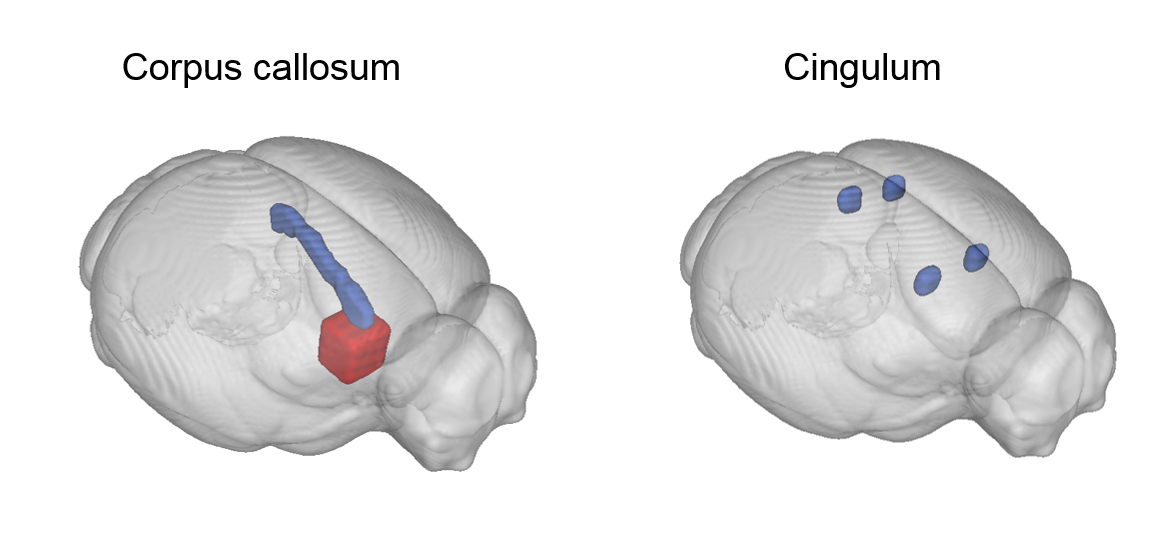
\includegraphics[scale=0.7]{figures/cntnap2_figure_s3.png}
    \decoRule
    \caption[Location of waypoint ROIs used for virtual dissection of
    corpus callosum and cingulum tracts from whole-brain white matter
    tractography.]{Location of waypoint ROIs used for virtual dissection of
    corpus callosum and cingulum tracts from whole-brain white matter
    tractography. Inclusion ROIs are indicated in blue, exclusion ROIs are
    indicated in red.}
    \label{fig:cntnap2_figs3}
\end{figure}

\subsection{Rabies virus production and injection}

Unpseudotyped recombinant SAD$\Delta$G-mCherry rabies virus (RV) was produced as
described by \textcite{osakada2013}. Briefly, B7GG packaging cells,
which express the rabies envelope G protein, were infected with unpseudotyped
SAD$\Delta$G-mCherry-RV, obtained by courtesy of Prof. Edward Callaway from the Salk
Institute. After five to six days, the virus was collected, filtrated with 0.45
$\mu m$ filter and concentrated by two rounds of ultracentrifugation. The titer of
the SAD$\Delta$G-mCherry-RV preparation was established by infecting Hek-293T cells
(ATCC cat no. CRL-11268) with tenfold serial dilution of viral stock, counting
mCherry expressing cells 3 days after infection. The titer was calculated as
2x1011 Infective Units (IU)/ml, and the stock was therefore considered suitable
for in vivo microinjection. Intracortical rabies virus injections were carried
out as previously described \parencite{sforazzini2016} in adult (12-16 week-old)
male \textit{Cntnap2}$^{-/-}$ and control \textit{Cntnap2}$^{+/+}$ littermates (n = 6, each group). To this
purpose, mice were deeply anesthetized with avertin (250 mg/kg) and firmly
stabilized on a stereotaxic apparatus (Stoelting Inc.). A micro drill (Cellpoint
Scientific Inc.) was used to drill holes through the skull. Injections were
performed with a Nanofil syringe mounted on an UltraMicroPump UMP3 with a four
channel Micro4 controller (World Precision Instruments), at a speed of 5 nl/s,
followed by a 5–10 minutes waiting period, to avoid backflow of viral solution
and unspecific labelling. One $\mu l$ of viral stock solution was injected
unilaterally in the left anterior prefrontal cortex using the following
coordinates for injections, expressed in mm from bregma: 1.42 from anterior to
posterior, 0.3 lateral, -1.6 deep \parencite{paxinos2004} 

\subsection{Quantification of retrogradely labelled cells}

RV-labelled cell quantification and histological analyses where carried out by
an operator (A.B.) blind to genotype. After 7 days from viral injection, the
animals were transcardially perfused with 4 \% paraformaldehyde (PFA), brains
were dissected, post-fixed over night at $4\degree$C and vibratome-cut (Leica
Microsystems).  RV-infected cells were detected by means of immunohistochemistry
performed on every other 100 $\mu m$ thick coronal section, using rabbit anti-red
fluorescent protein (RFP) primary antibody (1:500, AbCam), and goat anti-rabbit
HRP secondary antibody (1:500, Jackson ImmunoResearch), followed by 3-3’
diaminobenzidine tetrahydrochloride (DAB, Sigma Aldrich) staining. Imaging was
performed with MacroFluo microscope (Leica). Each picture was then superimposed
onto the corresponding Paxinos Atlas table \parencite{paxinos2004}, and cell
bodies were plotted according to their anatomical localization. The cells were
then assigned to their corresponding brain regions, and final region-based cell
population counts were expressed as fraction of the total amount of labelled
cells.

\subsection{Histological and immunohistochemical analysis of white matter}

To histologically assess the presence of microstructural white matter
alterations, we examined immunofluorescence-enhanced coronal brain sections
covering anterior callosal regions from adult (12 week-old) male \textit{Cntnap2}$^{-/-}$ and
control \textit{Cntnap2}$^{+/+}$ littermates (n = 5, each group) after incubation with rat
anti-myelin basic protein (MBP) primary antibody (1:1000, AbCam), followed by
donkey anti-rat 594 secondary antibody (1:500, Thermo scientific). We also
quantified MBP levels as previously described \parencite{mottershead2003,
richetto2017}.  Briefly, three representative random images in anterior callosal
regions characterized by parallel or transversal fiber extension with respect to
the image plane (corpus callosum and forceps minor of the corpus callosum,
respectively) were acquired on a Nikon A1 confocal system, equipped with 561
laser diode and appropriate filter for Texas Red fluorophore. Z-stack images
(1.5 $\mu m$ thick) were acquired using an oil-immersion 60x plan-apochromat
objective at 1024x1024 pixel resolution. Callosal image fields were also
qualitatively inspected for the presence of inter-group differences in white
matter organization or reduced neuronal packing/density. MBP content was
empirically quantified by summing MBP-immunoreactive areas expressed as number
of pixels whose values were above the background threshold, calculated as pixel
intensity values in areas with no detectable immunostaining, such as cell nuclei
or MBP-devoid background.

\section{Results}

\subsection{Reduced local and long-range connectivity in fronto-cortical regions
of \textit{Cntnap2}$^{-/-}$ mice}

To obtain an unbiased mapping of genotype-dependent differences in functional
connectivity, we implemented recently developed aggregative metrics for local
and long-range functional connectivity. This analysis revealed foci of
significantly reduced local and long-range connectivity in \textit{Cntnap2}$^{-/-}$ mutants
with respect to wild-type control subjects (t-test, p < 0.05 FWE
cluster-corrected, with cluster-defining threshold of t24 > 2.06, p < 0.05;
Fig.~\ref{fig:cntnap2_fig01}) encompassing prefrontal (prelimbic and cingulate)
and retrosplenial cortices.  These same brain regions have been classified both
in mice and in humans as “high strength” functional connectivity hubs
\parencite{buckner2009, cole2010, liska2015}, and as such are thought to play a
key integrative role in distributed functional networks. Local connectivity
reductions appeared to be more widespread than corresponding long-range
connectivity deficits (Fig.~\ref{fig:cntnap2_fig01}a, c), encompassing
involvement of supplementary motor areas surrounding cingulate cortex. The
observed local and long-range connectivity reductions were statistically
significant also when integrated over a large volume of interest encompassing
the whole cingulate cortex (local connectivity: Cg, t-test, t24 = 3.11, p =
0.005, Fig.~\ref{fig:cntnap2_fig01}b; long-range connectivity: Cg, t-test, t24 =
2.26, p = 0.03, Fig.~\ref{fig:cntnap2_fig01}d). 

\begin{figure}[th] 
    \centering
    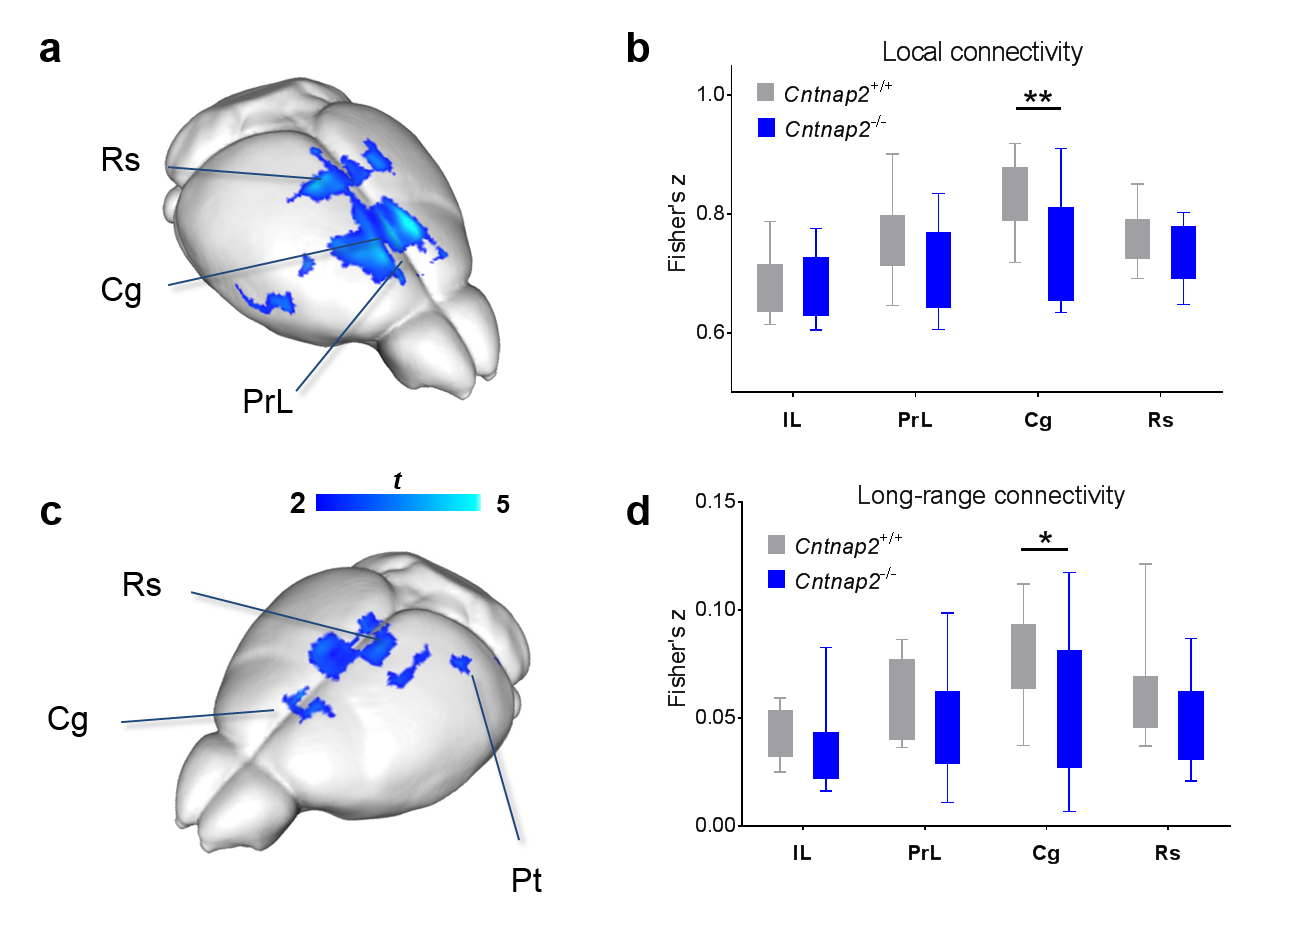
\includegraphics[scale=0.6]{figures/cntnap2_figure_01.png}
    \decoRule
    \caption[Reduced local and long-range connectivity in \textit{Cntnap2}$^{-/-}$
    mutants.]{Reduced local and long-range connectivity in \textit{Cntnap2}$^{-/-}$ mutants.
    (\textbf{a}) Foci of reduced local connectivity in \textit{Cntnap2}$^{-/-}$ vs. control
    \textit{Cntnap2}$^{+/+}$ littermates (t-test; t24 > 2.06, p < 0.05; cluster corrected with
    cluster-level p < 0.05). (\textbf{b}) Mean local connectivity in regions of
    interest (t-test; Cg: t24 = 3.11, p = 0.005). (\textbf{c}) Foci of reduced
    long-range connectivity in \textit{Cntnap2}$^{-/-}$ vs. control \textit{Cntnap2}$^{+/+}$ littermates
    (t-test; p < 0.05 FWE cluster-corrected, with cluster-defining threshold of
    t24 > 2.06, p < 0.05). (\textbf{d}) Mean long-range connectivity in regions
    of interest (t-test; Cg: t24 = 2.26, p = 0.03). IL, infra-limbic cortex;
    PrL, prelimbic cortex, Cg, cingulate cortex; Rs, retrosplenial cortex, * p <
    0.05, **p < 0.01.}
    \label{fig:cntnap2_fig01}
\end{figure}


\subsection{Long-range connectivity impairments in \textit{Cntnap2}$^{-/-}$ mice affect
heteromodal cortical regions and the DMN}

To identify regional targets of the observed long-range connectivity deficits,
we probed rsfMRI networks previously shown to involve prefrontal, cingulate and
retrosplenial regions \parencite{sforazzini2014, gozzi2016}. Seed-based mapping
of retrosplenial and anterior cingulate/prelimbic cortex highlighted foci of
reciprocal long-range hypoconnectivity along the midline brain axis in
\textit{Cntnap2}$^{-/-}$ mutants (t-test, p < 0.05 FWE cluster-corrected, with
cluster-defining threshold of t24 > 2.06, p < 0.05;
Fig.~\ref{fig:cntnap2_fig02}a, b). We also probed connectivity of putative
lateral components of the rodent DMN such as the posterior parietal and temporal
association/auditory cortices, and postero-ventral hippocampus
\parencite{gozzi2016}. Parietal cortical mapping revealed foci of reduced local
and long-range (middle cingulate) connectivity in \textit{Cntnap2}$^{-/-}$ mice (t-test, p <
0.05 FWE cluster-corrected, with cluster-defining threshold of t24 > 2.06, p <
0.05; Fig.~\ref{fig:cntnap2_fig02}c). In the same animals, temporal association
areas appeared to be widely hypo-connected to retrosplenial, cingulate and
prefrontal regions (t-test, p < 0.05 FWE cluster-corrected, with
cluster-defining threshold of t24 > 2.06, p < 0.05;
Fig.~\ref{fig:cntnap2_fig02}d). We also observed foci of long-range
hypo-connectivity between ventral hippocampal and ventral prefrontal
(infralimbic) regions (t-test, p < 0.05 FWE cluster-corrected, with
cluster-defining threshold of t24 > 2.06, p < 0.05;
Fig.~\ref{fig:cntnap2_fig02}e). Inter-hemispheric connectivity in subcortical or
motor-sensory networks appeared to be overall largely preserved. A reduction in
inter-hemispheric connectivity was observed in primary motor areas and visual
cortex when quantified in anatomical volumes of interest
(Fig.~\ref{fig:cntnap2_figs4}), although the effect did not survive false
discovery rate correction.

\begin{figure}[th] 
    \centering
    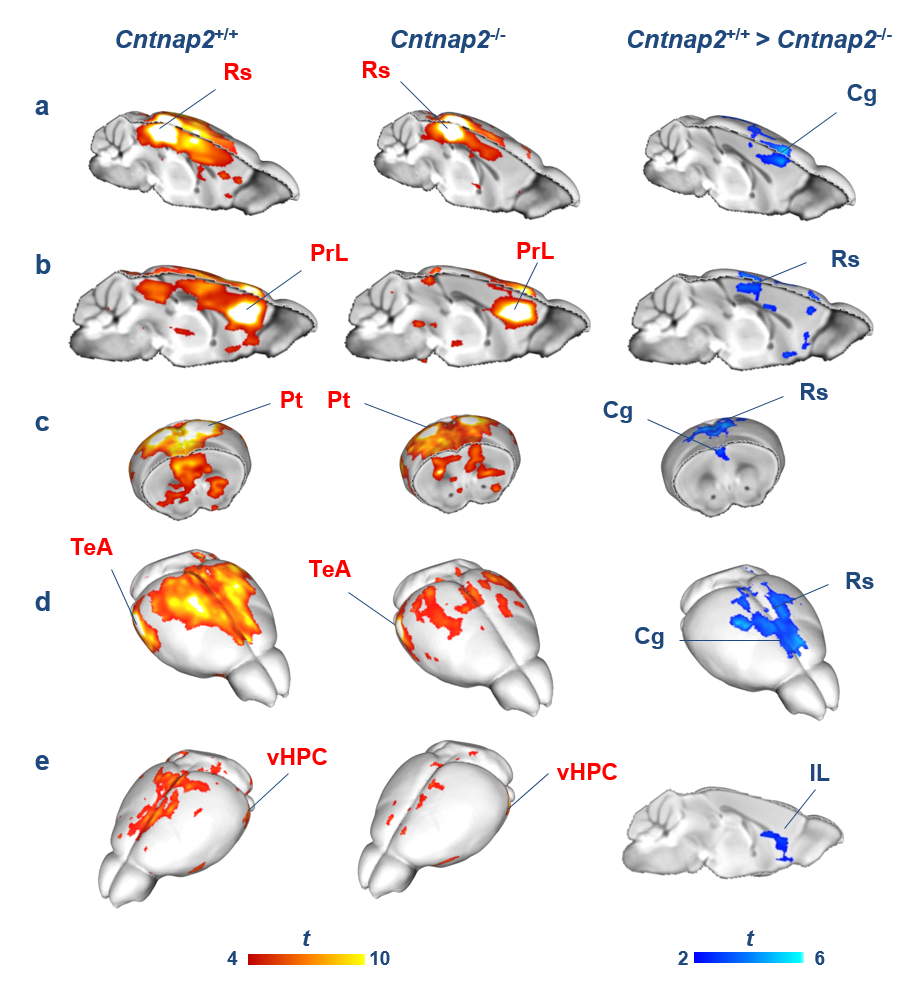
\includegraphics[scale=0.7]{figures/cntnap2_figure_02.png}
    \decoRule
    \caption[Reduced long-range connectivity in \textit{Cntnap2}$^{-/-}$ mice.]{Reduced
    long-range connectivity in \textit{Cntnap2}$^{-/-}$ mice. (\textbf{a}-\textbf{e})
    Seed-correlation mapping highlighted convergent reduced connectivity between
    long-range cortical and subcortical regions and cingulate-prefrontal areas.
    Red/yellow shows areas with significant correlation with seed regions
    indicated in red (one-sample t-test, p < 0.05 FWE cluster corrected with
    cluster-defining threshold of t12 > 2.18, p < 0.05). Blue indicates foci of
    reduced connectivity in \textit{Cntnap2}$^{-/-}$ mutants with respect to control mice
    (t-test, p < 0.05 FWE cluster corrected with cluster-defining threshold of
    t24 > 2.06, p < 0.05).  Rs, retrosplenial cortex; IL, infra-limbic cortex;
    PrL, prelimbic cortex; Cg, cingulate cortex; Rs, retrosplenial cortex; vHPC,
    ventral hippocampus; Au/TeA, auditory/temporal association cortices; Pt,
    parietal cortex.}
    \label{fig:cntnap2_fig02}
\end{figure}

\begin{figure}[th] 
    \centering
    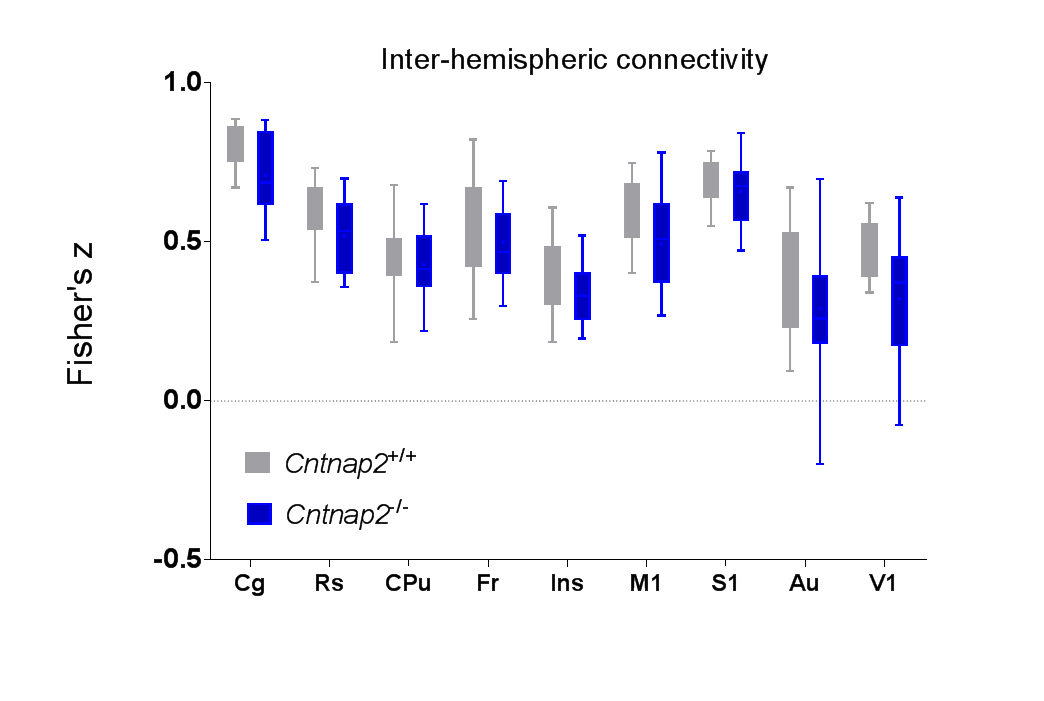
\includegraphics[scale=0.7]{figures/cntnap2_figure_s4.png}
    \decoRule
    \caption[Largely preserved inter-hemispheric connectivity in \textit{Cntnap2}$^{-/-}$
    mutants and control mice.]{Largely preserved inter-hemispheric connectivity
    in \textit{Cntnap2}$^{-/-}$ mutants and control mice. Correlation coefficients were
    calculated between time courses extracted from VOIs depicted in
    Fig.~\ref{fig:cntnap2_figs1} and the resulting r-scores were transformed to
    z-scores using Fisher’s r-to-z transform. None of these comparisons
    survived a false discovery rate correction at q = 0.05. }
    \label{fig:cntnap2_figs4}
\end{figure}

Importantly, no genotype-dependent differences in anaesthesia sensitivity were
detected as seen with mean arterial blood pressure mapping (t-test, t24 = 0.17,
p = 0.87; Fig.~\ref{fig:cntnap2_figs5}a) and amplitude of cortical BOLD signal
fluctuations (t-test, t24 = 0.72, p = 0.48; Fig.~\ref{fig:cntnap2_figs5}b), two
independent readouts previously shown to be linearly correlated with anaesthesia
depth \parencite{steffey2003, liu2011}.  Together with the observation of
region-dependent alterations, as opposed to the global reduction described with
increased anaesthesia dosing \parencite{nasrallah2014}, these findings strongly
argue against a confounding contribution of anaesthesia to the observed
hypo-connectivity. 

\begin{figure}[th] 
    \centering
    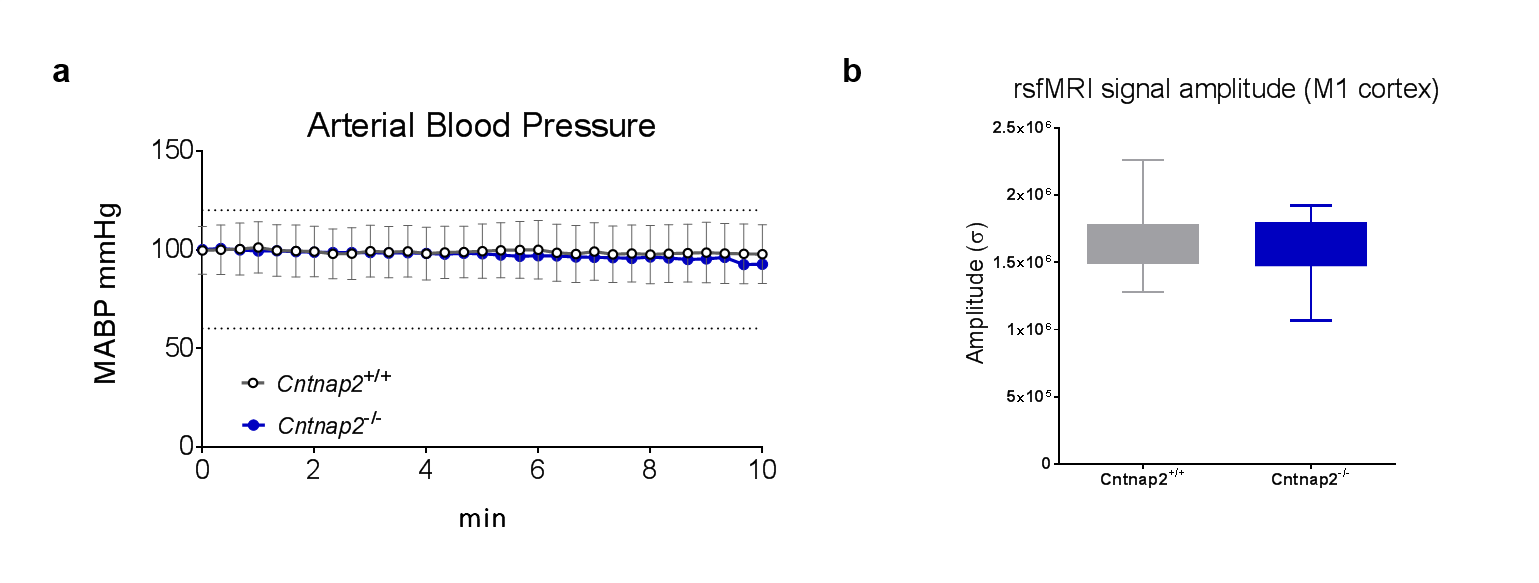
\includegraphics[scale=0.55]{figures/cntnap2_figure_s5.png}
    \decoRule
    \caption[No genotype-dependent differences in anaesthesia sensitivity in
    \textit{Cntnap2}$^{-/-}$ mice.]{No genotype-dependent differences in anaesthesia
    sensitivity were detected as seen with mean arterial blood pressure mapping
    (t-test, t24 = 0.17, p = 0.87; a) and amplitude of cortical BOLD signal
    fluctuations in primary motor cortex (t-test, t24 = 0.72, p = 0.48; b). M1,
    primary motor cortex.}
    \label{fig:cntnap2_figs5}
\end{figure}

\subsection{Hypoconnectivity in the mouse DMN is associated with impaired social
behaviour}

Recent human imaging studies in socially-impaired patients have revealed a
putative association between long-range DMN hypo-connectivity and social
competence \parencite{schreiner2014}. Based on these findings, we hypothesized
that reduced long-range DMN connectivity in \textit{Cntnap2}$^{-/-}$ mice could be associated
with impaired social behaviour. To test this hypothesis, we first corroborated
DMN hypoconnectivity by quantifying functional connectivity along the dorsal
midline axis of this network (anterior/middle cingulate cortex and
retrosplenial cortex) using multiple seed-to-VOI measurements
(Fig.~\ref{fig:cntnap2_fig03}). A clear dysconnection between posterior
(retrosplenial) and middle/anterior portions of the DMN (cingulate, prelimbic
cortex) was apparent (retrosplenial to cingulate cortex: two-way
repeated-measures ANOVA, genotype effect, F1,24 = 5.76, p = 0.02,
Fig.~\ref{fig:cntnap2_fig03}a; retrosplenial-cingulate to prelimbic: two-way
repeated-measures ANOVA, genotype effect, F1,24 = 6.82, p = 0.02,
Fig.~\ref{fig:cntnap2_fig03}b). 

\begin{figure}[th] 
    \centering
    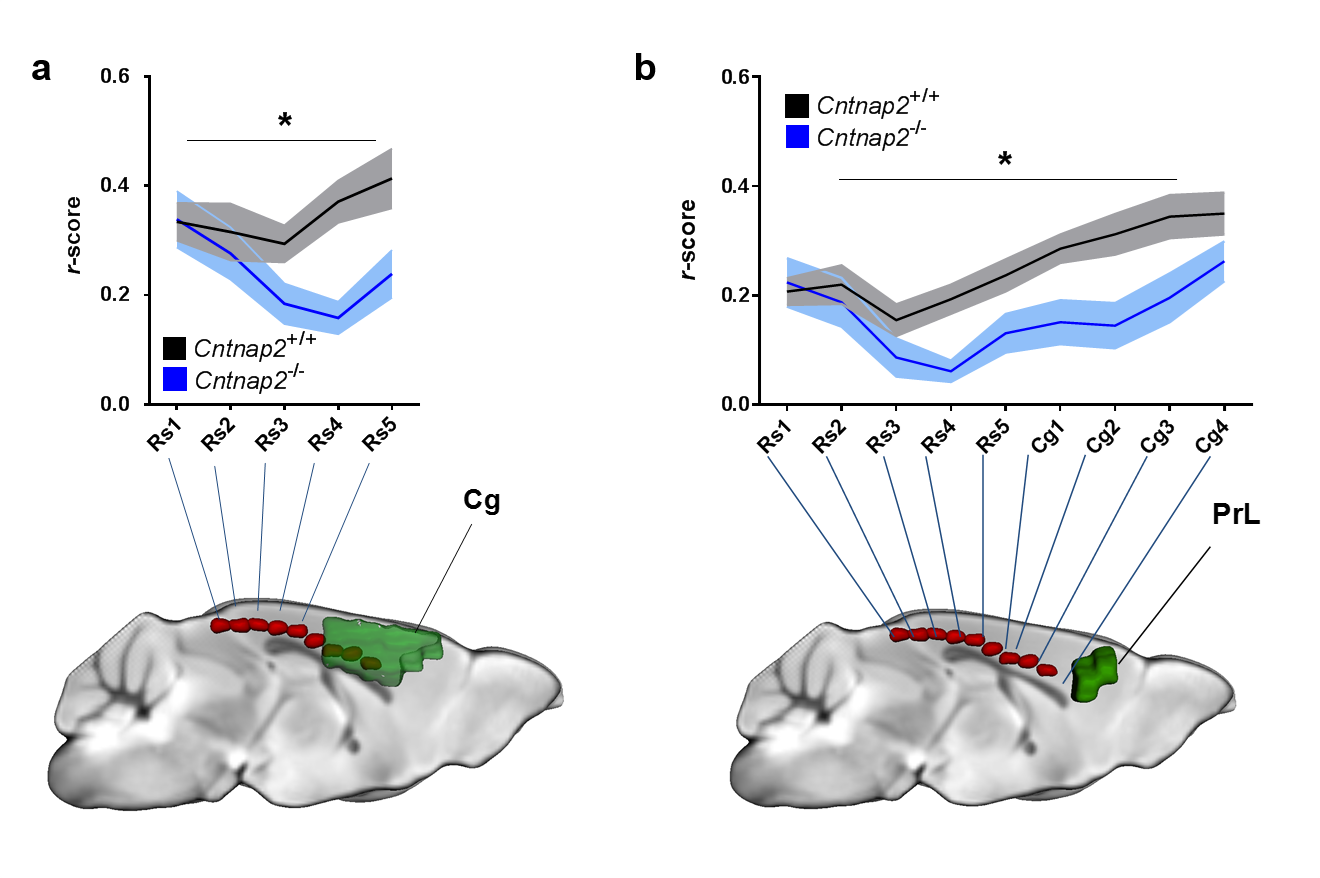
\includegraphics[scale=0.6]{figures/cntnap2_figure_03.png}
    \decoRule
    \caption[Fronto-posterior hypoconnectivity in \textit{Cntnap2}$^{-/-}$
    mice.]{Fronto-posterior hypoconnectivity in \textit{Cntnap2}$^{-/-}$ mice. (\textbf{a})
    Connectivity profile between a series of retrosplenial seeds (Rs, red) and
    the cingulate cortex (Cg, green) (two-way repeated-measures ANOVA, genotype
    effect, F1,24 = 5.76, p = 0.02). (\textbf{b}) Connectivity profile between a
    series of retrosplenial/cingulate seeds (Rs, Cg, red) and the prelimbic
    cortex (PrL, green) (two-way repeated-measures ANOVA, genotype effect, F1,24
    = 6.82, p = 0.02). * p < 0.05.}
    \label{fig:cntnap2_fig03}
\end{figure}

We then measured social behaviour in adult \textit{Cntnap2}$^{-/-}$ and \textit{Cntnap2}$^{+/+}$ control
mice in a male-female interaction test, and correlated the measured social
scores with DMN hypoconnectivity measures. Consistent with previous reports
\parencite{penagarikano2011}, behavioural testing revealed significantly
impaired social interest (total sniffing, duration: t-test, t24 = 2.29, p =
0.03, Fig.~\ref{fig:cntnap2_fig04}a; social investigation, duration: t-test, t24
= 2.43, p = 0.02, Fig.~\ref{fig:cntnap2_fig04}c) and increased non-social
behaviour (wall-rearing, frequency: t-test, t24 = 3.09, p = 0.01;
Fig.~\ref{fig:cntnap2_figs6}a) in \textit{Cntnap2}$^{-/-}$ mutants compared to \textit{Cntnap2}$^{+/+}$
control littermates. Hypo-connectivity in key DMN components
(retrosplenial-cingulate cortex) was significantly associated with reduced
social behaviour (total sniffing, duration: r = 0.42, p = 0.03, n = 26, R2 =
0.17, Fig.~\ref{fig:cntnap2_fig04}b; social investigation, duration: r = 0.40, p
= 0.04, n = 26, R2 = 0.16, Fig.~\ref{fig:cntnap2_fig04}d) and increased
non-social behaviour (wall rearing, frequency: r = -0.45, p = 0.02, n = 26, R2 =
0.21; Fig.~\ref{fig:cntnap2_figs6}b). These findings highlight a correlation
between fronto-posterior connectivity and social behaviour, suggesting that
impaired functional couplings produced by mutations in \textit{Cntnap2} could reverberate
to affect complex behavioural traits such as sociability and social exploration.

\begin{figure}[th] 
    \centering
    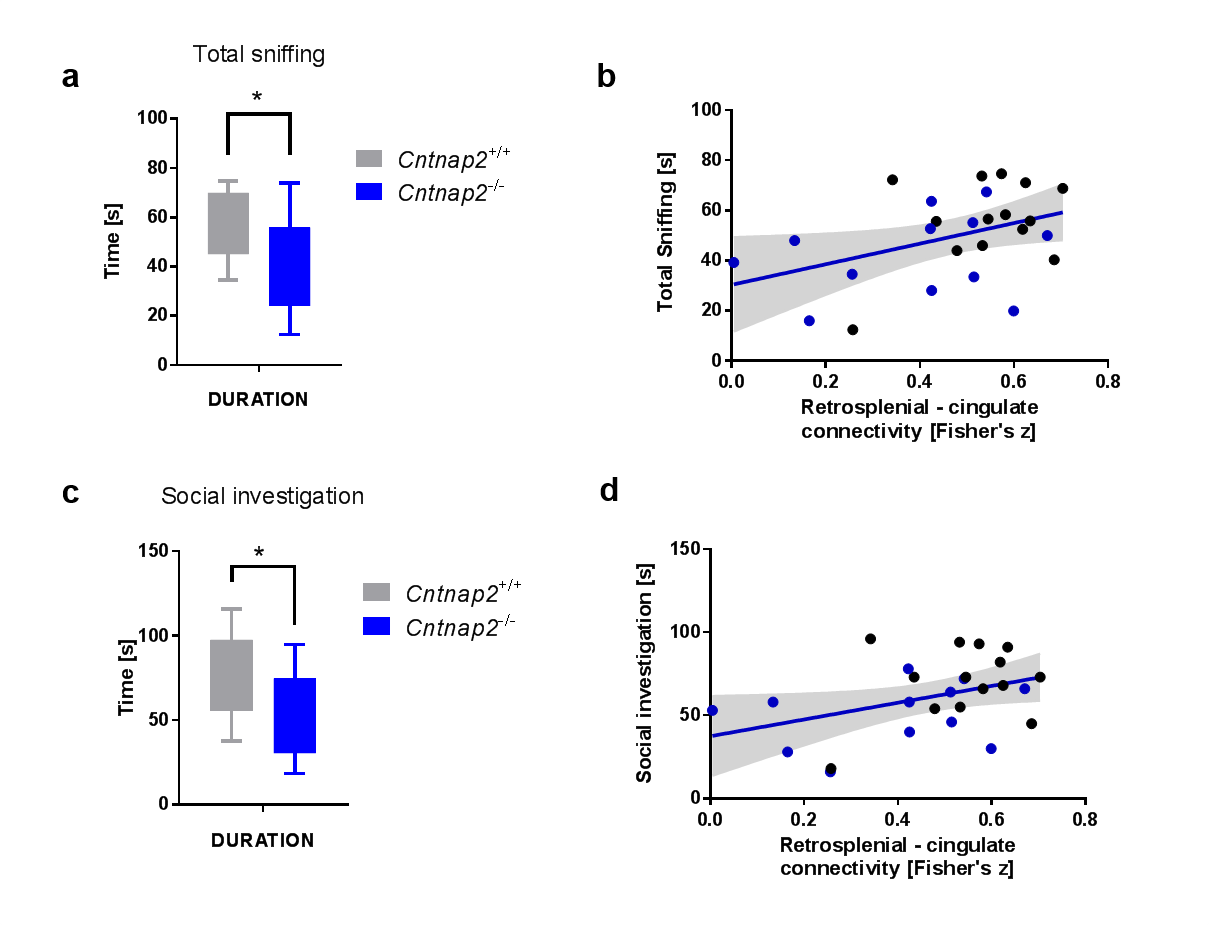
\includegraphics[scale=0.7]{figures/cntnap2_figure_04.png}
    \decoRule
    \caption[Fronto-posterior connectivity is correlated with social
    behaviour.]{Fronto-posterior connectivity is correlated with social
    behaviour.  (\textbf{a}) Social behaviour as measured by total sniffing
    duration (t-test, t24 = 2.29, p = 0.03). (\textbf{b}) Association between
    retrosplenial-cingulate connectivity (VOI to VOI) and total sniffing
    duration (r = 0.42, p = 0.03, n = 26, R2 = 0.17). (\textbf{c}) Social
    behaviour as measured by the duration of social investigation (t-test, t24 =
    2.43, p = 0.02). (\textbf{d}) Association between retrosplenial-cingulate
    connectivity (VOI-to-VOI) and the duration of social investigation (r =
    0.40, p = 0.04, n = 26, R2 = 0.16). * p < 0.05.}
    \label{fig:cntnap2_fig04}
\end{figure}

\begin{figure}[th] 
    \centering
    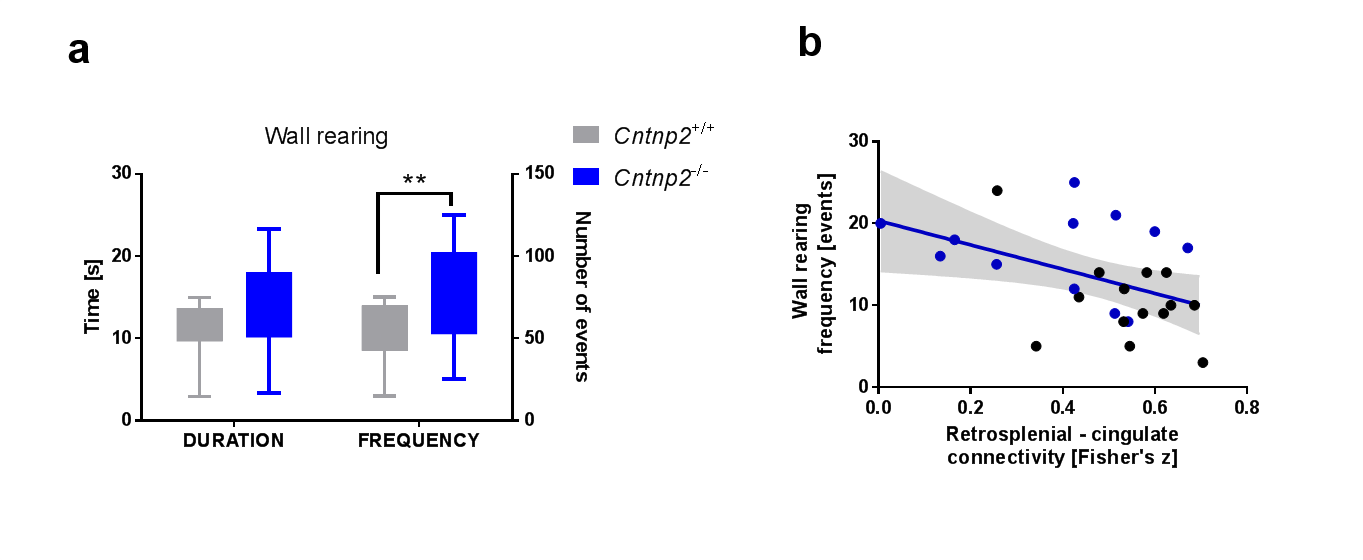
\includegraphics[scale=0.65]{figures/cntnap2_figure_s6.png}
    \decoRule
    \caption[Increased non-social behaviour in \textit{Cntnap2}$^{-/-}$ mutants compared to
    control littermates.]{Increased non-social behaviour in \textit{Cntnap2}$^{-/-}$ mutants
    compared to control littermates. (\textbf{a}) Non-social behaviour as
    measured by the duration and frequency of rearing up against the wall of the
    home-cage (frequency: t-test, t24 = 3.09, p = 0.01). (\textbf{b}) An inverse
    association between non-social behaviour and connectivity between
    retrosplenial and cingulate cortices (wall rearing, frequency: r = -0.45, p
    = 0.02, n = 26, R2 = 0.21). * p < 0.05, ** p < 0.01.}
    \label{fig:cntnap2_figs6}
\end{figure}

\subsection{Macroscale cortico-cortical white matter connectivity is preserved
in \textit{Cntnap2}$^{-/-}$ mice}

To probe a role of macroscale anatomical connectivity alterations on the
observed functional decoupling in \textit{Cntnap2}$^{-/-}$, we performed tractography analysis
of the corpus callosum and cingulum, two major white matter tracts characterised
by extensive cortico-cortical antero-posterior extension
(Fig.~\ref{fig:cntnap2_fig05}a). These white matter tracts appeared to be
largely typical in mutant and control mice as seen with group-level fibre
density maps (Fig.~\ref{fig:cntnap2_fig05}b); in keeping with this, we did not
observe statistically significant differences in the number of streamlines
between \textit{Cntnap2}$^{-/-}$ mutants and controls (cingulum: t-test, t21 = 1.25, p = 0.23;
corpus callosum: t-test, t21 = 1.21, p = 0.24; Fig.~\ref{fig:cntnap2_figs7}).
These results argue against a contribution of gross macroscale white matter
alterations to the observed functional connectivity impairments.

\begin{figure}[th] 
    \centering
    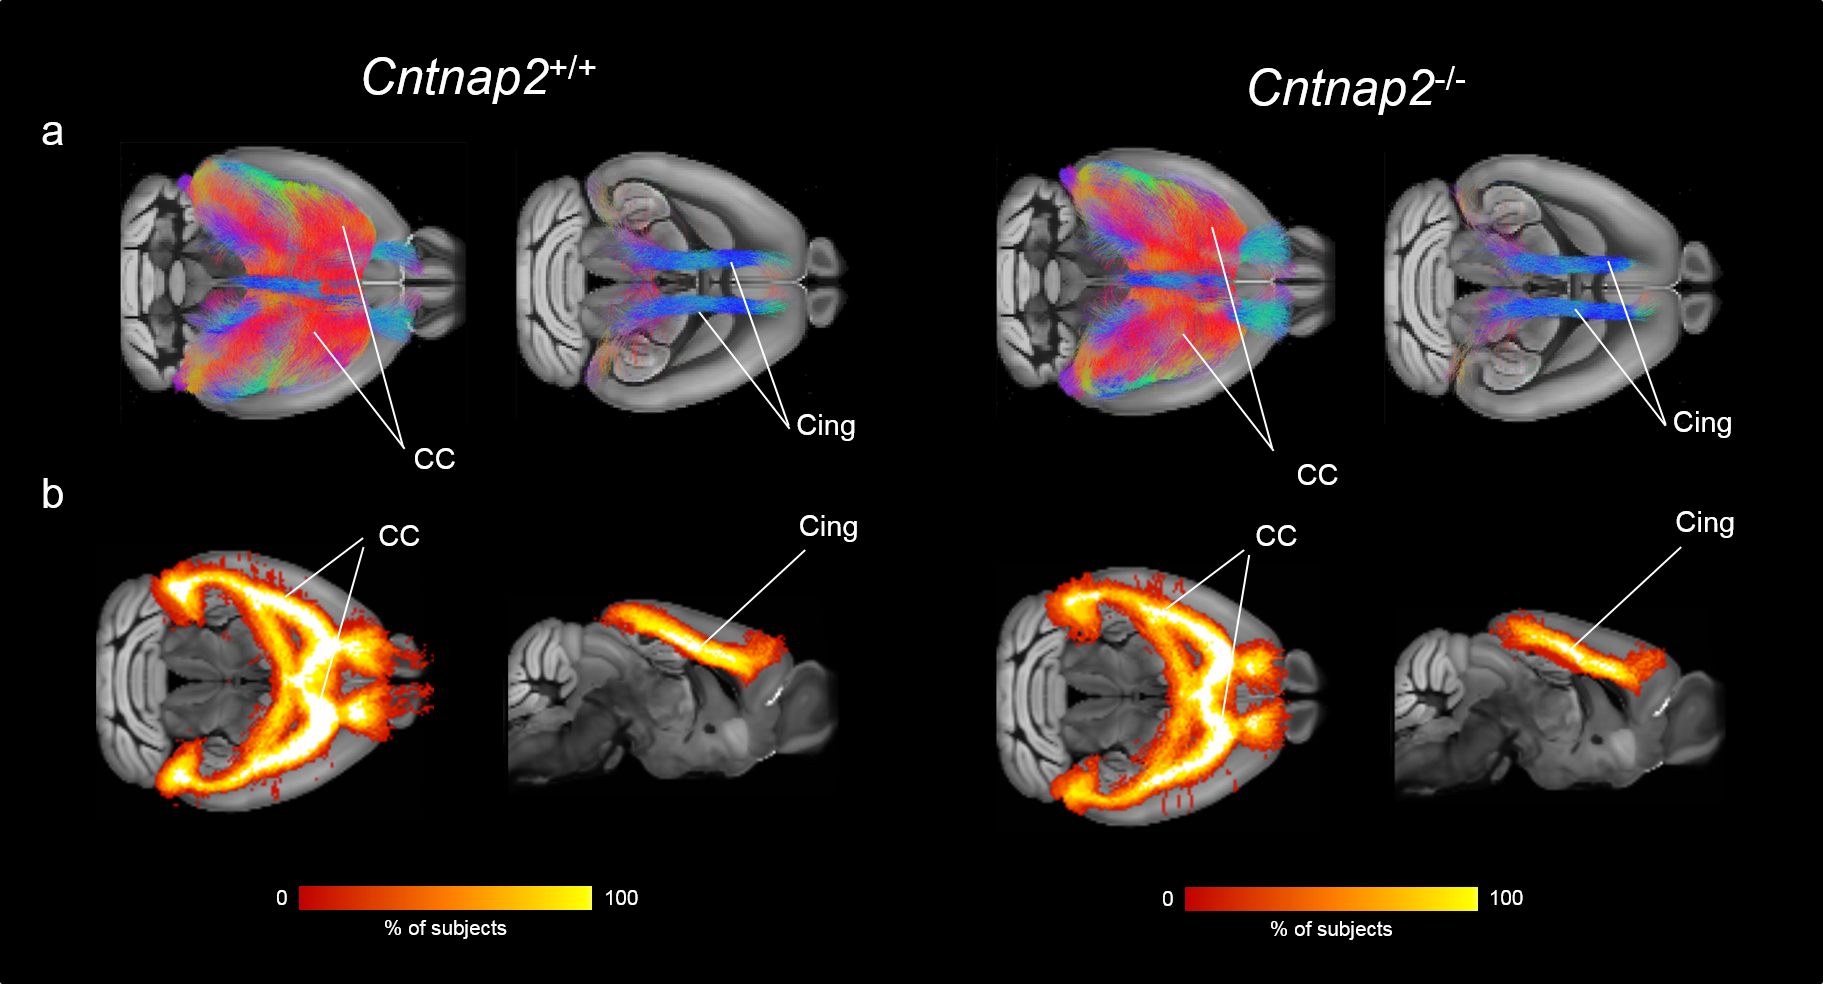
\includegraphics[scale=0.45]{figures/cntnap2_figure_05.png}
    \decoRule
    \caption[Preserved cortico-cortical white matter organization
    in \textit{Cntnap2}$^{-/-}$ mutants.]{Preserved cortico-cortical white matter organization
    in \textit{Cntnap2}$^{-/-}$ mutants. (\textbf{a}) Corpus callosum and cingulum tracts virtually
    dissected in two representative subjects (\textit{Cntnap2}$^{+/+}$ left, \textit{Cntnap2}$^{-/-}$
    right), (\textbf{b}) Fractional group fibre density maps for corpus callosum and
    cingulum tracts (\textit{Cntnap2}$^{+/+}$ left, \textit{Cntnap2}$^{-/-}$, right).}
    \label{fig:cntnap2_fig05}
\end{figure}

\begin{figure}[th] 
    \centering
    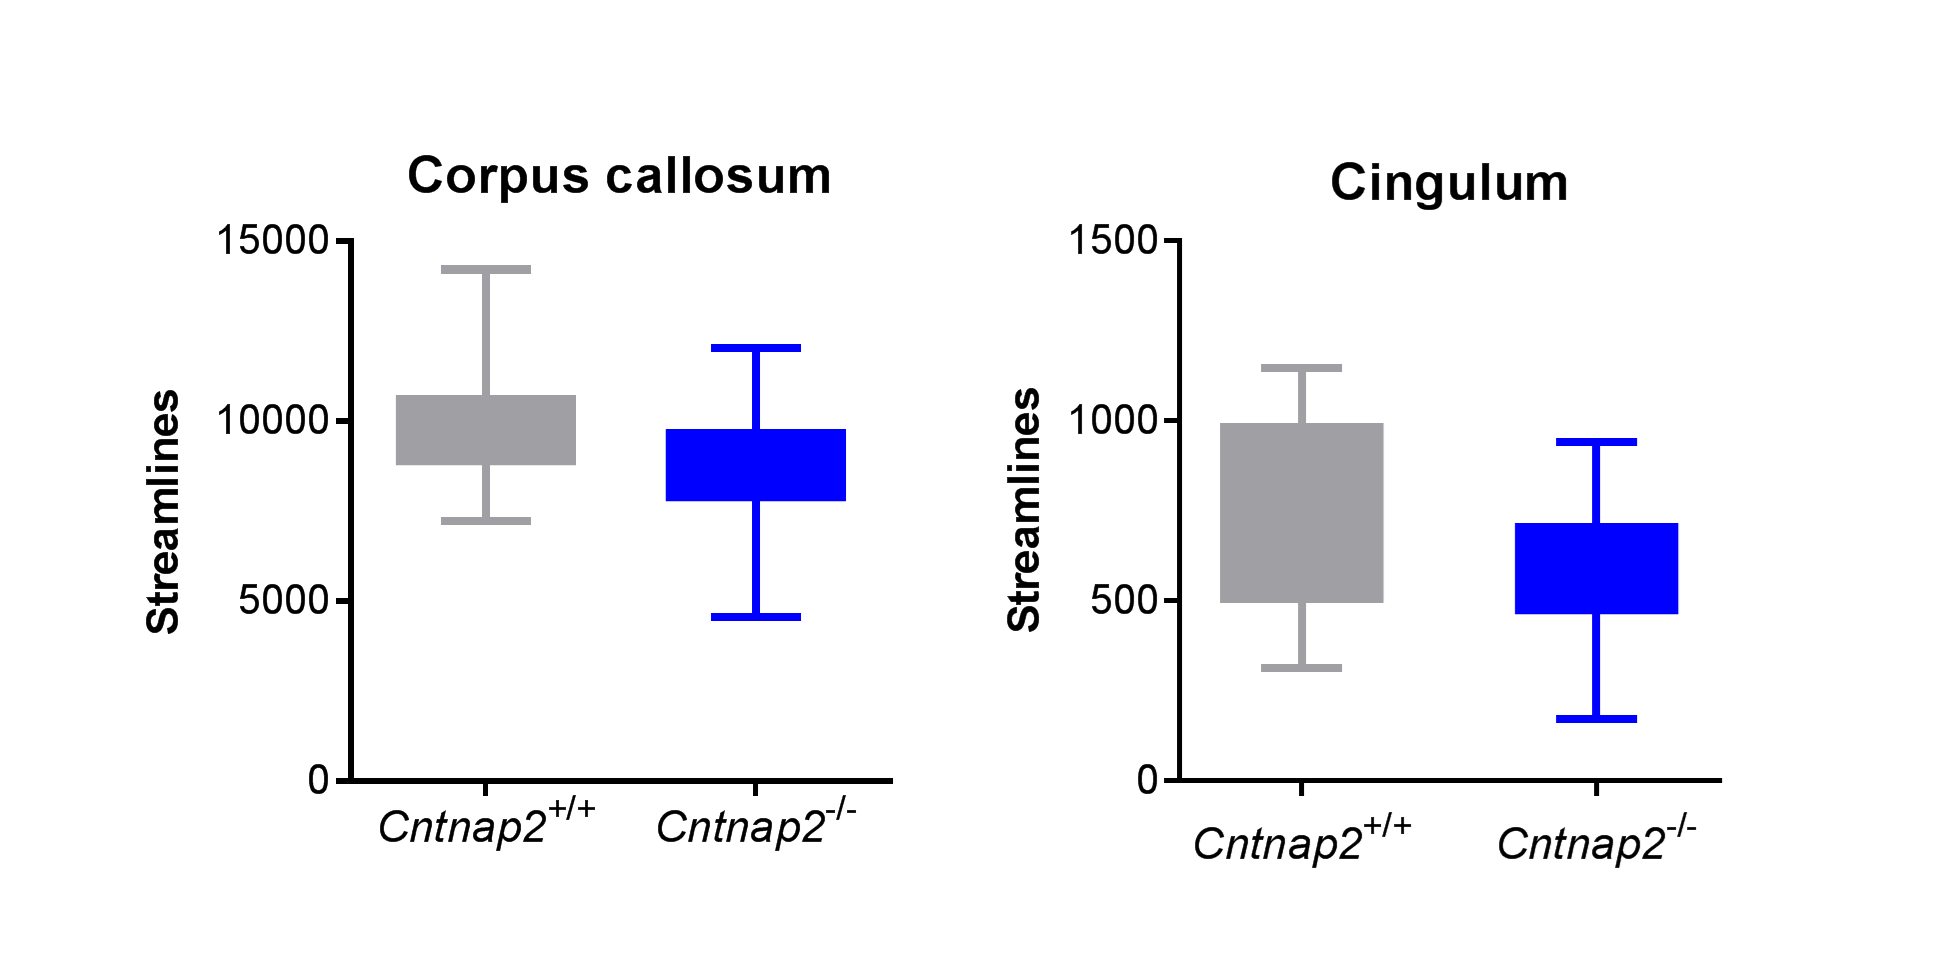
\includegraphics[scale=0.4]{figures/cntnap2_figure_s7.png}
    \decoRule
    \caption[White-matter tractography-based streamline counts.]{White-matter
    tractography-based streamline counts.  Numbers of streamlines in corpus
    callosum and cingulum showed no significant differences between the
    \textit{Cntnap2}$^{-/-}$ and control littermates (cingulum: t-test, t21 = 1.25, p = 0.23;
    corpus callosum: t-test, t21 = 1.21, p = 0.24).}
    \label{fig:cntnap2_figs7}
\end{figure}

\subsection{Reduced prefrontal-projecting neuronal clusters in cingulate cortex
of \textit{Cntnap2}$^{-/-}$ mice}

Although macroscale cortico-cortical connectivity appeared to be normal in
\textit{Cntnap2}$^{-/-}$ mutants, the possibility exists that finer-scale miswiring,
undetectable by tractography, may contribute to the mapped functional
connectivity alterations. To probe this hypothesis, we carried out monosynaptic
retrograde tracing of the left prefrontal cortex [prelimbic/anterior cingulate
cortex area 1, corresponding to Brodmann area 24Ab, \parencite{vogt2014}] and
quantified the number of retrogradely labelled cells in representative volumes
of interest in mutant and control littermate mice
(Fig.~\ref{fig:cntnap2_fig06}a). The anatomical distribution of retrogradely
labelled neurons in both genotypes was in keeping with previously published
rodent studies \parencite{hoover2007} and encompassed several key anatomical
substrates considered to be part of the rodent DMN \parencite{gozzi2016}.
Notably, regional quantification of the relative fraction of labelled cells
revealed reduced frequency of prefrontal-projecting neurons in the cingulate
cortex of \textit{Cntnap2}$^{-/-}$ mutants (Cg: t-test, t10 = 3.90, p = 0.003, FDR-corrected p
= 0.04; Fig.~\ref{fig:cntnap2_fig06}b, c). Importantly, no genotype-dependent
significant difference in the number of prefrontal projecting neurons was
observed in any of the other cortical or subcortical regions examined
(Fig.~\ref{fig:cntnap2_fig06}c).

\begin{figure}[th] 
    \centering
    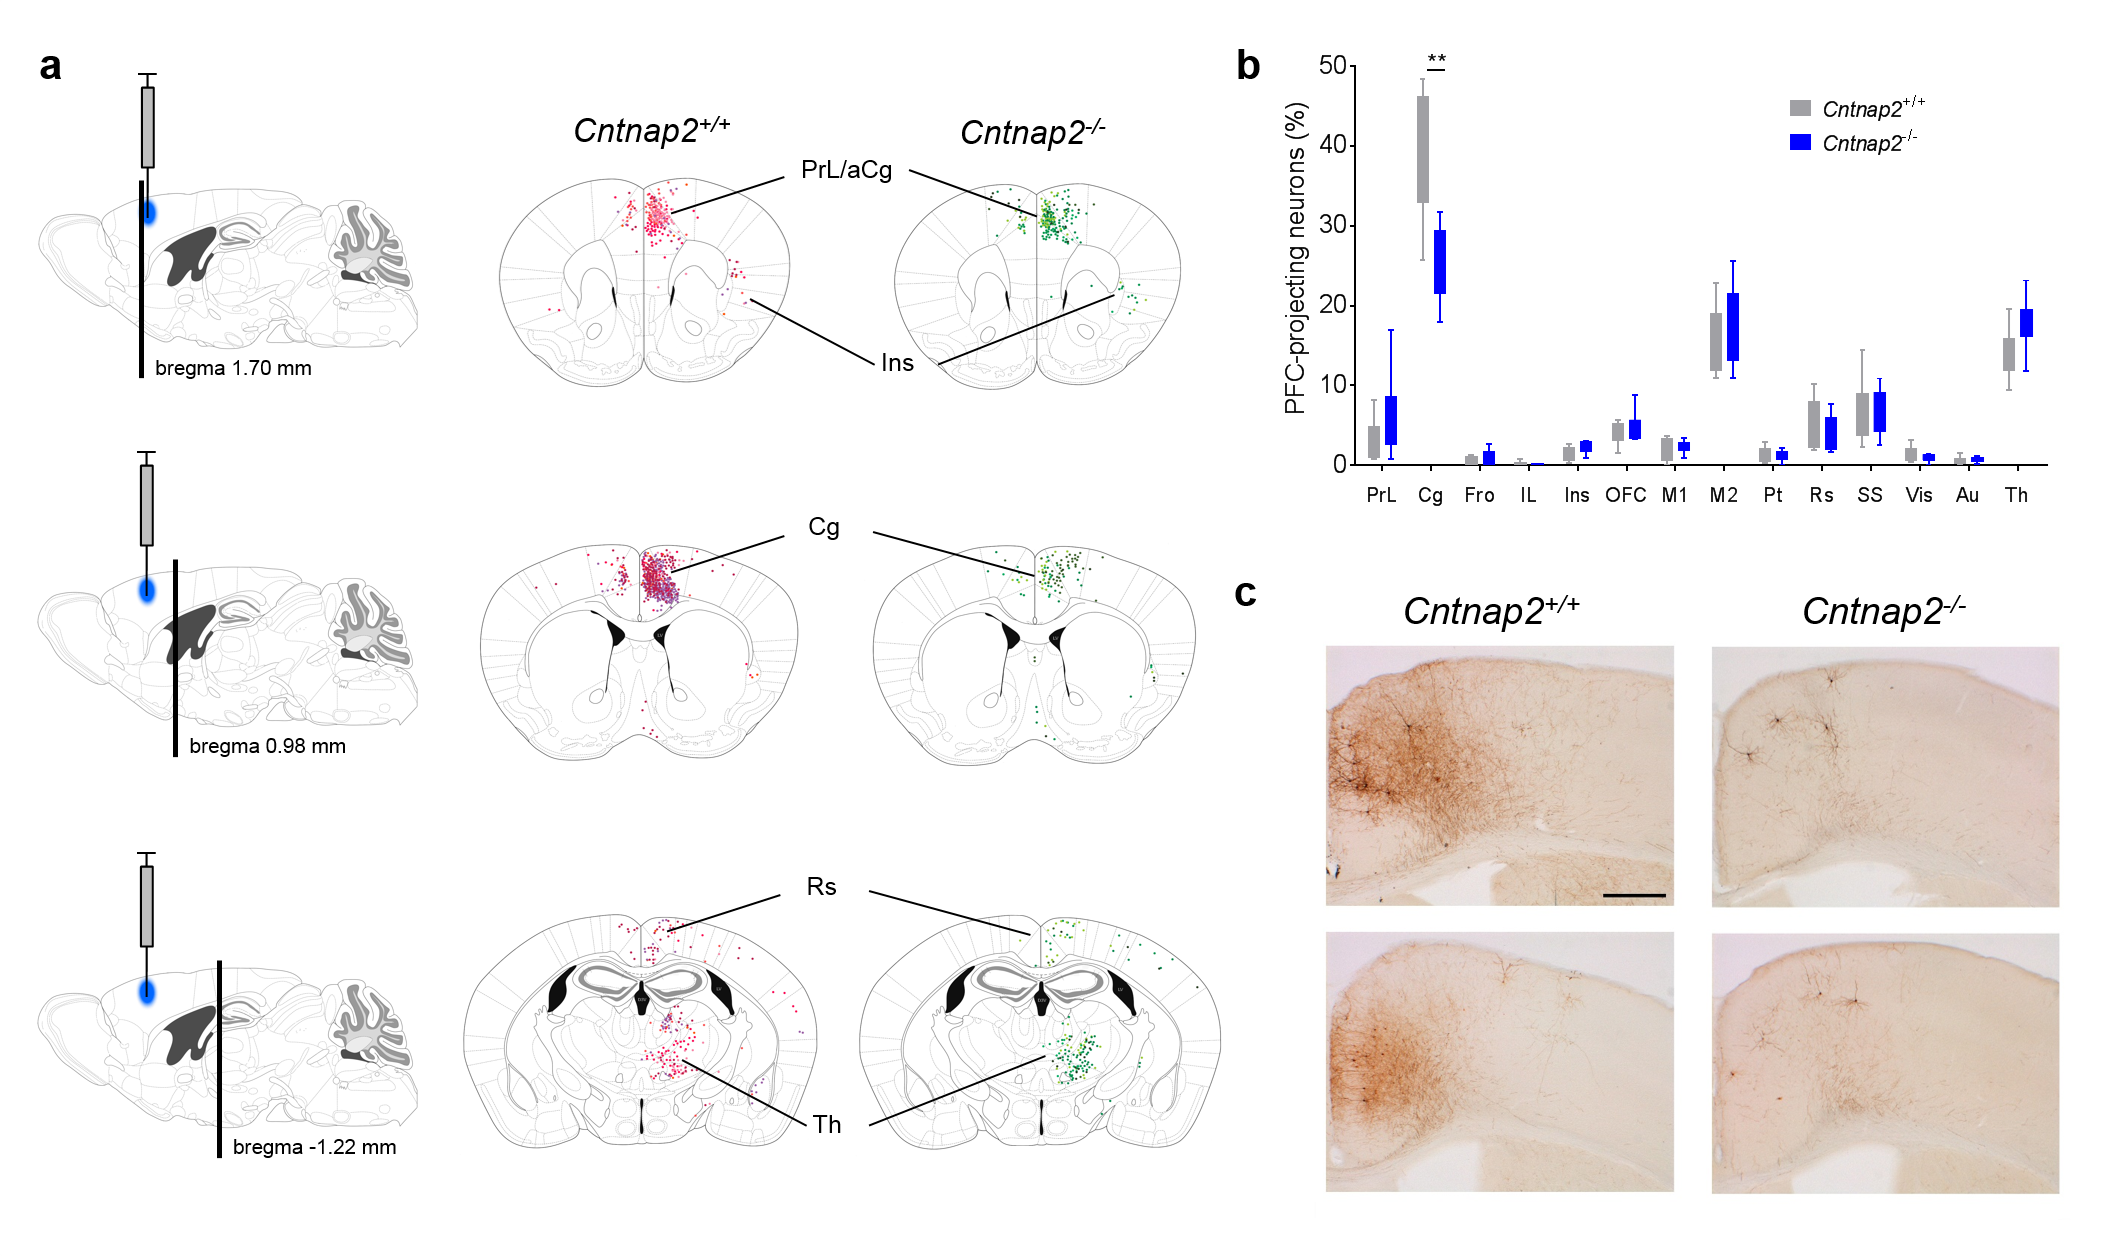
\includegraphics[scale=0.4]{figures/cntnap2_figure_06.png}
    \decoRule
    \caption[Reduced frequency of cingulate-prefrontal projecting neurons in
    \textit{Cntnap2}$^{-/-}$ mice.]{Reduced frequency of cingulate-prefrontal projecting
    neurons in \textit{Cntnap2}$^{-/-}$ mice. (\textbf{a}) Locations of retrogradely labelled
    cells superimposed on the corresponding Paxinos Atlas coronal tables.
    Injection location is indicated in blue on the sagittal tables. (\textbf{b})
    Regional quantification of the relative regional number (frequency) of
    retrogradely labelled cells (t-test; Cg: t10 = 3.90, p = 0.003,
    FDR-corrected p = 0.04). (\textbf{c}) Enlarged view of the distribution of
    retrogradely labelled cells in a coronal section of the cingulate region
    (bregma 0.98 mm) in two representative \textit{Cntnap2}$^{+/+}$ and two \textit{Cntnap2}$^{-/-}$
    subjects. The scale bar indicates 250 um. * p < 0.05, ** p < 0.01.}
    \label{fig:cntnap2_fig06}
\end{figure}

\subsection{Preserved microscale white matter organization in \textit{Cntnap2}$^{-/-}$ mice}

We next examined the presence of microscale white matter structural
abnormalities in control and \textit{Cntnap2}$^{-/-}$ mutants via histological examinations
and myelin binding protein (MBP) quantification. In keeping with previous
investigations \parencite{poliak2003, penagarikano2011}, we did not observe
gross microscale white matter disorganization or morphological changes in mice
lacking \textit{Cntnap2} with respect to control littermates
(Fig.~\ref{fig:cntnap2_figs8}a). Similarly, MBP quantification in frontal
callosal white matter tracts did not reveal any significant between-group
difference (corpus callosum: t-test, t8 = 0.84, p = 0.42; forceps minor of the
corpus callosum: t-test, t8 = 1.06, p = 0.32; Fig.~\ref{fig:cntnap2_figs8}b).

\begin{figure}[th] 
    \centering
    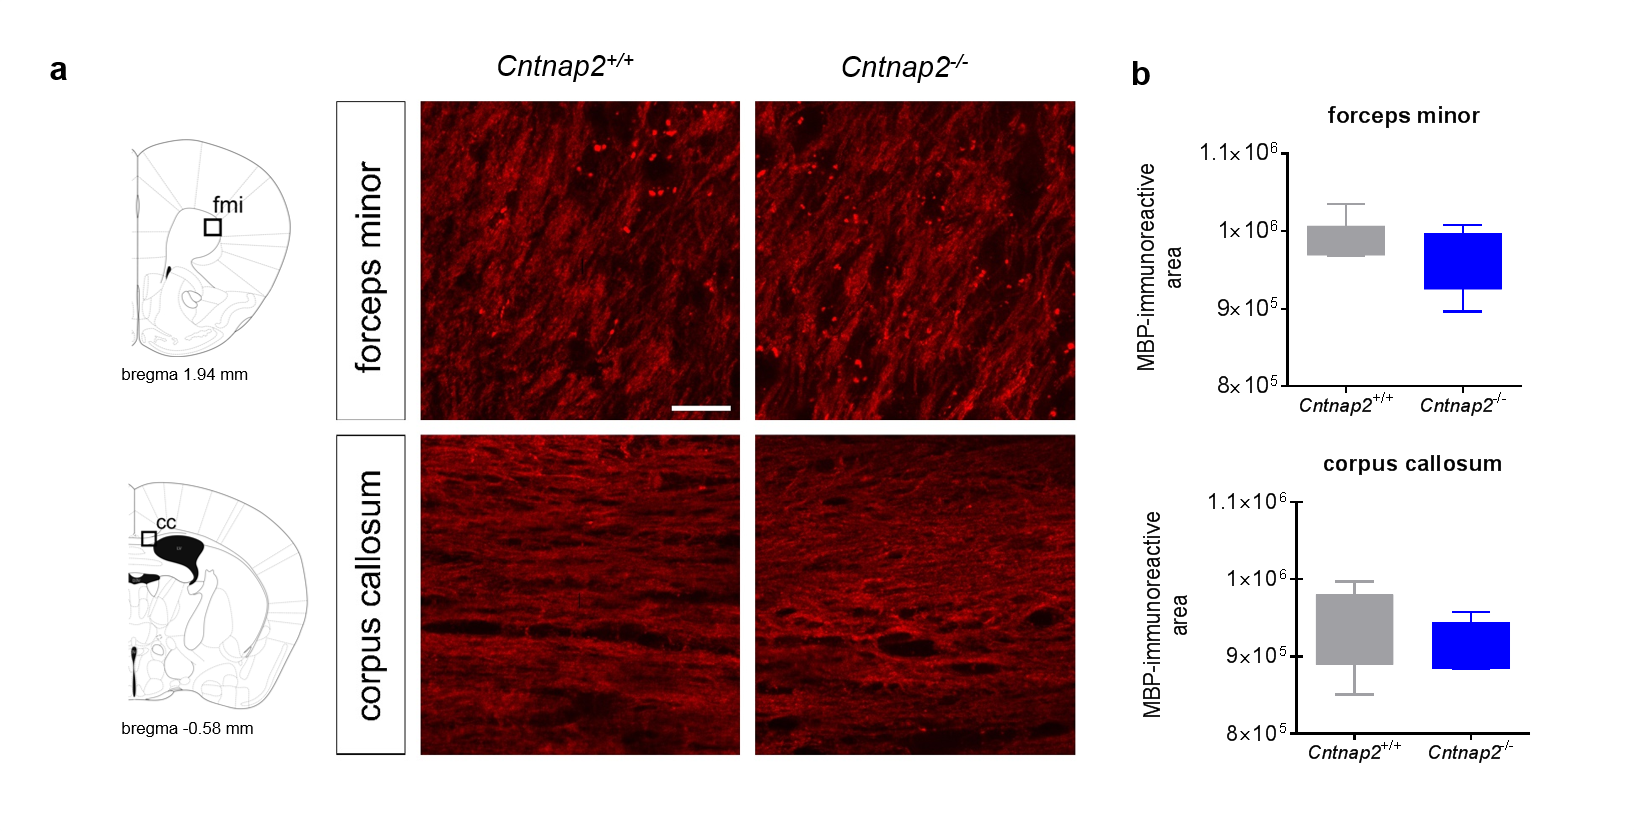
\includegraphics[scale=0.5]{figures/cntnap2_figure_s8.png}
    \decoRule
    \caption[Histological and immunohistochemical analysis of white
    matter.]{Histological and immunohistochemical analysis of white matter.
    (\textbf{a}) Representative images of anterior callosal regions
    characterized by parallel or transversal fibre extension with respect to the
    imaging plane (corpus callosum and forceps minor of the corpus callosum,
    respectively). No apparent difference in fibre organization or MBP stained
    regions was observed between genotypes. (\textbf{b}) MBP-immunoreactive area
    averaged from three random image fields per region and animal (n = 5, each
    group; corpus callosum: t-test, t8 = 0.84, p = 0.42; forceps minor of the
    corpus callosum: t-test, t8 = 1.06, p = 0.32).}
    \label{fig:cntnap2_figs8}
\end{figure}

\section{Discussion}

Here we show that homozygous mice lacking \textit{Cntnap2}, a neurexin superfamily member
associated with autism, exhibit reduced long-range and local functional
connectivity in prefrontal cortical regions and midline functional hubs of the
mouse brain, an effect that may involve defective cingulate-prefrontal mesoscale
wiring. We also show that reduced fronto-posterior connectivity is associated
with impaired social behaviour, revealing a possible link between long-range
functional connectivity alterations and mouse behavioural traits recapitulating
ASD symptoms. Collectively, these findings suggest that loss-of-function
mutations in \textit{Cntnap2} may predispose to neurodevelopmental disorders and autism
through dysregulation of macroscale functional network couplings.

Our use of an imaging readout widely employed in human connectivity mapping
provides us with the opportunity to cross-compare connectivity findings across
species. In this respect, the observation of long-range fronto-posterior
hypo-connectivity in \textit{Cntnap2}$^{-/-}$ mice is especially noteworthy, because it is in
excellent agreement with the results of a recent human imaging study where an
association between common genetic variants in CNTNAP2 and similar long-range
frontal hypoconnectivity was described \parencite{scott-vanzeeland2010}. Our
results expand these findings, by revealing a causal contribution of \textit{Cntnap2}
loss-of-function mutations to long-range fronto-cortical connectivity
impairments. These correspondences also serve as an important proof-of-concept
demonstration that ASD-related genetic mutations can lead to comparable
macroscale connectivity deficits in humans and lower mammal species like the
laboratory mouse. The presence of long-range hypoconnectivity in \textit{Cntnap2}$^{-/-}$ mice
also adds to the remarkable construct and face validity of this mouse model as
an experimental tool for mechanistic and therapeutic investigation of syndromic
forms of ASD \parencite{penagarikano2011}. Specifically, \textit{Cntnap2}$^{-/-}$ mice closely
recapitulate major neuropathological features observed in cortical
dysplasia-focal epilepsy (CDFE) syndrome, a rare neuronal migration disorder
associated with a recessive (suggesting loss of function) mutation in CNTNAP2,
and, in nearly two thirds of patients, with autism \parencite{strauss2006}.
These include behavioural deficits in the three core domains of ASD (reduced
vocal communication, repetitive and restricted behaviours, and abnormal social
interactions), hyperactivity and epileptic seizures (both features described in
CDFE patients), and reduced GABAergic interneurons, resulting in asynchronous
cortical activity as measured with in vivo two-photon calcium imaging
\parencite{penagarikano2011}.

The observation of defective mesoscale axonal wiring in the cingulate cortex
corroborates the presence of selective prefrontal dysregulation in \textit{Cntnap2}$^{-/-}$
mutants, and serves as a possible neuroanatomical correlate for some of the
prefrontal functional connectivity impairments mapped with rsfMRI. Regional
differences in GABAergic interneuron density, and developmental processes
related to circuit and network refinements \parencite{zhan2014, riccomagno2015}
are, however, likely to play a role in the observed functional desynchronization
as well, given the established contribution of GABAergic oscillatory rhythms in
mediating large-scale functional synchrony \parencite{gonzalez-burgos2008} and
the recent evidence of altered spine density and increased spine eliminations in
\textit{Cntnap2}$^{-/-}$ mice \parencite{gdalyahu2015}. The relative contribution of
anatomical versus neurophysiological mechanisms in determining the observed
desynchronization remains however undetermined, and interventional studies
entailing the regional manipulation of excitatory/inhibitory ratio or
inactivation of projection-specific pathways may be required to disambiguate
this issue.

Recent human studies described possible microstructural white matter
alterations in carriers of CNTNAP2 mutations as assessed with water diffusion
anisotropy.  Specifically, gender-dependent reductions in fractional anisotropy
(FA) in the inferior fronto-occipital fasciculus or anterior thalamic radiation
have been described by \textcite{tan2010}. Similarly,
\textcite{clemmvonhohenberg2013} described an interaction between a single
genotype (rs2710126) and FA, in which homozygotes for the risk allele showed
reduced FA values in uncinate fasciculus. 

These preliminary results suggest the presence of possible white matter
microstructural alterations as a result of CNTNAP2 gene mutations. However,
anisotropic water diffusion reflects multiples biophysical contributions that
prevent an unequivocal microstructural interpretation of these findings. For
example, reduced FA could be the result of reduced neuronal packing,
myelinisation, axonal diameter, neuronal integrity and maturation, as well as
regional differences in gray matter fraction \parencite{beaulieu2009}. To
investigate potential microstructural white matter disruption at a more detailed
level than permitted by diffusion MRI, we carried out a histological assessment
of white matter fibres using MBP immunofluorescence. We did not observe any
gross white matter microstructural abnormality in \textit{Cntnap2}$^{-/-}$ mutants in terms of
fibre orientation, packing or organization. Moreover, MBP quantification did not
reveal any significant genotype-dependent differences. Together with previous
electron microscopy investigations, where normal myelin thickness was reported
in \textit{Cntnap2}$^{-/-}$ mutants \parencite{poliak2003}, these findings argue against the
presence of gross microscale white matter alterations in these mutants. While
this finding appears to be in contrast with human investigations of CNTNAP2
polymorphisms and suggestive of possible species-specific divergence, additional
research is required to more thoroughly investigate the presence of white matter
microstructural aberrancies in \textit{Cntnap2}$^{-/-}$ mutants. It should also be noted that
CNTNAP2 polymorphisms studies in humans are typically correlative and involve
small patient samples, which make them more prone to confounding factors related
to heterogeneity in clinical samples, and individual adaptive differences in
microstructural parameters \parencite{scholz2009}.

The observation of hypoconnectivity in prefrontal hub regions of the DMN
\parencite{liska2015} is suggestive of a deficient “maturation” of this
functional network (supekar2010), and is in keeping with the hypothesis of a key
role of this region as a mediator of deficits in global perception and its
cognitive representations in ASD patients \parencite{martinez-sanchis2014}. The
notion that “underconnectivity” may preferentially affect complex cognitive and
social functions and their high order cortical substrates rather than low-level
sensory and perceptual tasks has recently found some theoretical support
\parencite{kana2011}.  Within this framework, heteromodal integrative hubs like
the anterior cingulate and prefrontal cortex, as well as retrosplenial regions
would serve as major points of vulnerability for the stability of distributed
functional network couplings. rsfMRI mapping in additional mouse lines
harbouring ASD-related genetic mutations will be instrumental in assessing
whether the observed alterations represent a generalizable endophenotype that
may converge across mutations and genetic etiologies, or are the specific
consequence of \textit{Cntnap2} mutations. It is, however, interesting to note that so
far hypoconnectivity appears to be predominant in mouse imaging studies of ASD:
reduced connectivity in several brain regions including the prefrontal cortex
and the DMN has been observed in the BTBR model of idiopathic autism
\parencite{sforazzini2016}, and in mice characterised by reduced synaptic
pruning \parencite{zhan2014}, a pathological trait associated with autism
\parencite{tang2014}. Reduced connectivity between motor sensory regions and a
general reduction in primary visual cortex connectivity were also recently
described in a mouse model of fragile X syndrome (haberl2015). Although
preliminary, these initial mouse findings are consistent with and somehow
support the “under-connectivity theory” of autism, according to which reduced
functional connectivity, at least in the adult brain \parencite{uddin2013}, may
emerge as a dominant feature of ASD in the face of heterogeneous
etiopathological pathways \parencite{dimartino2014a, uddin2013}.

In contrast with our imaging results, human rsfMRI mapping in CNTNAP2 common
variant carriers revealed increased, instead of decreased, local connectivity in
lateral prefrontal regions (scott-van2010). The reason behind this discrepancy
is not clear, although several important experimental factors, including
methodological, species- and/or age-related differences may contribute to this
inconsistency. For example, local connectivity was found to be increased in
human lateral prefrontal areas, a region that does not have a clear
cyto-architectural correlate in rodents \parencite{vogt2014}. Moreover, our
study was performed in adult male subjects, while human mapping was carried out
in pre-pubertal subjects (mean age 12 years old), a discrepancy that could
account for the differences in local connectivity alterations. Indeed, a
dramatic reorganization of large-scale functional brain networks occurs during
childhood and late adolescence in humans, involving developmental shifts from
short-range to long-range connectivity, notably within fronto-insular and
cortico-subcortical networks [reviewed by \parencite{ernst2015}]. Moreover, an
age-related dichotomy has been suggested in ASD-related connectivity
aberrancies, with generally reduced intrinsic functional connectivity in
adolescents and adults with autism compared with age-matched controls, and
increased functional connectivity in younger children with the disorder
\parencite{uddin2013}. A similar age-related shift could therefore possibly
explain the discrepant direction of local connectivity observed in our study
with respect to the finding reported by \textcite{scott-vanzeeland2010} in
human pre-adolescent subjects. Longitudinal investigations of connectivity in
rodent genetic models of autism are highly warranted to enable empirical testing
of the developmental trajectory of ASD-related connectivity aberrancies across
development and network maturation \parencite{liska2016}. Finally, differences
in the nature of the investigated mutations should also not be neglected, as
the functional consequences of the genetic variants imaged by
\textcite{scott-vanzeeland2010} are unclear, and the possibility that not all
the imaged genetic variants are loss-of-function cannot be ruled out. 

We also note here that our study specifically addressed male mice only, owing to
the greater ASD incidence in this gender \parencite{lai2015}. While this choice
has the advantage of reducing within-group variation and subsequent increase in
statistical power of our measurements, this should be considered a limitation of
our study, as it does not permit to assess whether our findings can be
generalized to female carriers of \textit{Cntnap2} loss-of-function mutations. 

In conclusion, we document that the absence of \textit{Cntnap2} leads to functional
connectivity reductions and defective mesoscale wiring in prefrontal functional
hubs of the mouse brain, an effect associated with impaired social behaviour.
These findings suggest that loss-of-function mutations in \textit{Cntnap2} may predispose
to neurodevelopmental disorders and autism through selective dysregulation of
connectivity in integrative prefrontal areas, and provide a translational model
for investigating connectional perturbations in syndromic ASD forms.

\chapter{Mouse imaging and the autism connectivity chaos}

\label{Chapter04}

\begin{quote}
    This chapter has been published as:

    \longfullcite{liska2016}
\end{quote}

\section{The connectivity theory of autism: open questions and controversies}

Autism is a heterogeneous syndrome characterised by core behavioural features
including deficits in social communication and interaction, as well as
restricted, repetitive patterns of behaviour and interests
\parencite{association2013}.  Although a primary and unitary aetiology for
autism spectrum disorder (ASD) has not been identified, its high heritability
has been consistently documented, revealing a contribution of complex and highly
heterogeneous genetic mutations \parencite{geschwind2009, geschwind2015,
sanders2015}. Remarkably, although previously identified mutations, genetic
syndromes and de novo copy number variations (CNVs) account for about 10–20 \%
of ASD cases, none of these single known genetic causes accounts for more than
1–2 \% of cases [reviewed in \parencite{abrahams2008}]. The phenotypic
expression (i.e., “penetrance”) of these genetic components is also highly
variable, ranging from fully penetrant point mutations to polygenic forms with
multiple gene–gene and gene–environment interactions. Remarkable variability
exists also in the extent of cognitive and behavioural abnormalities presented
by affected individuals \parencite{lai2014, chang2015, georgiades2013}, making
heterogeneity a dominant theme for this group of disorders. 

The advent of non-invasive brain imaging raised hopes that such clinical
heterogeneity could be narrowed down to a small number of identifiable “imaging
endophenotypes” that could help ASD diagnosis, patient stratification, and
possibly provide clues as to the elusive aetiology of this group of disorders.
Unfortunately, the results of imaging studies have proven overall as variable as
the clinical manifestations of ASD \parencite{ecker2015, stanfield2008}. A
notable exception to this scenario was the initial observation of reduced
connectivity between brain regions in ASD patients, a finding first reported by
Horowitz and colleagues \parencite{horwitz1988} using PET, and later
corroborated by task-based \parencite{just2004} and resting-state fMRI (rsfMRI)
studies \parencite{assaf2010, cherkassky2006, kennedy2008}, which revealed
impaired long-range synchronization in spontaneous brain activity. Together with
evidence of reduced white matter connectivity detected with MRI [reviewed in
\parencite{anagnostou2011}], these observations form the basis of the so called
“under-connectivity theory of autism” \parencite{anagnostou2011, just2012},
according to which deficient long-range communication between brain regions may
underlie ASD symptoms and pathophysiology. However, recent imaging studies have
strongly challenged this view, highlighting a much more heterogeneous picture
[see \parencite{vasa2016} for a recent review]. For example, rsfMRI mapping in a
large cohort of patients has revealed the presence of concomitant hypo- and
hyper-connectivity \parencite{dimartino2014a}, although a clear prevalence of
hypo-connected regions was apparent. Similarly, widespread hyper-connectivity
during childhood has also been recently described \parencite{keown2013,
supekar2013, uddin2013}, suggesting a possible neurodevelopmental origin for
these alterations. More recently, the hypothesis that such conflicting findings
could reflect greater inter-subject variability in ASD patients than in
neurotypical controls (i.e. idiosyncratic connectivity) has been proposed
\parencite{hahamy2015}. A putative confounding contribution of ASD-related
motion and its effect on functional connectivity readouts is also the subject of
an open controversy in the imaging community \parencite{deen2012, power2015,
power2012, pardoe2016}. 

Collectively, the extensive literature published to date points at the presence
of major functional connectivity alterations in ASD populations, although the
identified regional patterns vary considerably across studies and patient
cohorts \parencite{ameis2015, bernhardt2016, ecker2014, ecker2015, kana2011,
muller2014, vasa2016}. Despite this rapidly accumulating evidence, many
fundamental questions as to the origin and significance of connectional
alterations in ASD remain unanswered. For one, the neurophysiological
underpinnings of these connectional aberrancies are largely unknown, and a
causal etiopathological contribution of specific genetic variants to impaired
connectivity in ASD remains to be firmly established. More broadly, it is
unclear whether these abnormalities are a causative or epiphenomenal consequence
of the disease, and whether their heterogeneous expression reflects cohort
effects, different genetic aetiologies or neurodevelopmental trajectories. The
exact relationship between connectivity alterations and the severity of ASD
manifestation remains also obscure, with the vast majority of the human
neuroimaging literature being focused on high functioning ASD cohorts
\parencite{vissers2012}. 

A deeper understanding of the origin and significance of these phenomena is
greatly complicated by our very limited understanding of the neurobiological
foundations of macro-scale neuroimaging readouts commonly employed in ASD
research, such as white matter microstructural parameters [e.g. fractional
anisotropy \parencite{owen2014}], or the elusive functional couplings underlying
rsfMRI-based functional connectivity. This has left us with a major explanatory
gap between mechanistic models of brain function at the cellular and
microcircuit level, and the emergence of macroscale functional activity in
health and pathological states such as those that are observed in autism. As a
result, we are currently unable to properly interpret and back-translate
clinical evidence of aberrant connectivity into interpretable neurophysiological
events/models that can help understand, diagnose or treat these disorders. It is
also becoming apparent that a full disambiguation of the multifactorial and
complex determinants of aberrant functional connectivity in ASD can only be
obtained through the combined use of refined clinical imaging methods and
multimodal-multiscale investigational approaches that currently can only be
applied in experimental animal models.

\section{Bridging the gap: functional connectivity mapping in mouse autism
models}

The identification of several high-confidence ASD-risk genes involved in
syndromic forms of autism \parencite{sanders2015} has been paralleled by the
generation of mouse lines recapitulating human mutations. Despite predictable
limitations in reliably modelling the full phenotypic spectrum of a complex (and
possibly only human) developmental disorder like ASD, mouse models can be
harnessed to understand how genetic alterations translate into relevant changes
in cells and circuits, and ultimately to identify points of convergence for
molecular pathways, cells, circuits, and systems that may result in a deeper
understanding of the pathophysiology of ASD and related behavioural deficits
\parencite{arguello2012, nelson2015, vasa2016}. For example, molecular
investigations in ASD mouse models have been instrumental in the identification
of a limited set of molecular pathways to which ASD-involved genes seem to
converge, including, among others, synaptogenesis, synaptic function, and
neuronal translational regulation [reviewed in
\parencite{delatorre-ubieta2016}]. This effort has been accompanied by the
development of ASD-relevant behavioural phenotyping assays, primarily targeted
at social, communication and repetitive behaviours \parencite{wohr2013, kas2014,
silverman2010, homberg2016}. Interestingly, many – but not all – models showed
autism-like traits, with manifestations ranging from repetitive behaviours to
reduced social communication (ultrasonic vocalizations) and social interest
[reviewed in \parencite{ellegood2015}]. However, despite the widespread
application and high face validity of ASD behavioural phenotyping, the
significance and translational relevance of mouse behavioural alterations to
human ASD remain debated \parencite{wohr2013}, and should be extrapolated with
caution. 

Recent advances in mouse rsfMRI mapping [reviewed in \parencite{gozzi2016}]
offer the opportunity of extending mouse modelling of ASD to the investigation
of the neurobiological underpinnings and etiopathological significance of
ASD-related connectivity aberrations. Specifically, improvements in MRI imaging
hardware, together with tighter control of physiological and motion artefacts
\parencite{ferrari2012, weber2006} have led to robust and reproducible
identification of homotopic rsfMRI networks covering known cortical and
subcortical systems in the mouse by several research groups
\parencite{mechling2014, nasrallah2014, sforazzini2014, shah2016, zerbi2015}.
Interestingly, distributed networks encompassing heteromodal prefrontal and
posterior cortical regions have also been identified \parencite{sforazzini2014,
shah2016, zerbi2015}, leading to the suggestive hypothesis of the presence of
evolutionary precursors of the human salience network and default mode network
(DMN) in this species [reviewed in \parencite{gozzi2016}]. This notion is
empirically corroborated by the recent observation that
cytoarchitecturally-homologue regions such as anterior cingulate and
retrosplenial cortices \parencite{vogt2014} similarly serve as connectivity hubs
in humans and mice \parencite{cole2010, liska2015, tomasi2011}. Moreover, the
application of rsfMRI to the mouse brain comes with several important
advantages, including the possibility to use quantitative imaging modalities for
an objective endo-phenotypic characterization of ASD-related pathology
complementary to behavioural assays, and to validate its readouts with invasive
techniques that are off limits for human research, including local field
potentials (LFPs) coherence mappings \parencite{zhan2014}, local injection of
neuronal tracers \parencite{sforazzini2016}, as well as an ever-increasing array
of histopathological, stereological or immunohistochemical post-mortem analyses.

Collectively, these correspondences strongly support the use of rsfMRI as a
means to bridge research of functional connectivity aberrancies in autism across
species (man vs. mouse) and levels of inquiry (from cellular- and microscale to
meso- and macroscale, Fig.~\ref{fig:autism_fig01_bridge}), along two main
investigational routes. First, rsfMRI can be used to establish causal (rather
than associative) etiopathological contributions between specific ASD-associated
genetic variants and macroscale connectivity, thus complementing analogous
clinical research efforts using imaging genetics \parencite{rudie2012,
scott-vanzeeland2010}. One notable experimental advantage of mouse imaging with
respect to current human imaging genetic approaches is the possibility of
mapping and comparing the effect of multiple mutations (via the use of different
autism mouse models) under rigorously controlled experimental conditions, thus
reducing the confounding contribution of experimental variables that can be only
minimally controlled in human research, such as genetic and environmental
variability, age \parencite{uddin2013}, ASD-related motion, and group
differences in cognitive states \parencite{vasa2016}. The main goal of this line
of investigation is to assess whether seemingly unrelated ASD-risk mutations do
converge on a limited number of distinct functional connectivity endophenotypes.
An elegant demonstration of this approach has been recently described using
morpho-anatomical MRI. Brain-volumetric phenotypes of 26 ASD mouse models using
structural MRI methods exhibited clustering into three main groups, each with a
distinct set of concomitant changes in size across different brain regions
\parencite{ellegood2015a}. Such reduction of morpho-anatomical heterogeneity is
not surprising, given the wide (and sometimes opposing) stream of
pathophysiological alterations observed in syndromic forms of autism, which
range from basic molecular or synaptic mechanism such as protein synthesis
\parencite{geschwind2007, auerbach2011} up to homeostatic regulations of
excitatory and inhibitory neurotransmission \parencite{nelson2015}. Analogous
analyses with regards to functional connectivity phenotypes should be possible
in the future to associate basic pathophysiological traits with macroscale
connectional aberrancies. 

\begin{figure}[th] \centering
    \includegraphics[scale=0.75]{figures/autism_figure_01_bridge.png}
    \decoRule
    \caption[Mouse imaging can bridge
    the gap between microscale models of brain function, and clinical research
    of macroscale functional connectivity.]{Mouse imaging can bridge
    the gap between microscale models of brain function, and clinical research
    of macroscale functional connectivity. Mouse models provide a powerful
    reductive platform that can be employed to link etiological determinants of
    ASD, such as syndromic mutation or neurodevelopmental traits, to basic
    molecular and cellular signatures of pathology (left, top to down). However,
    until recently we have been unable to use this approach to study the
    neurobiological underpinnings of macroscale functional connectivity, owing
    to difficulty in translating models of brain function across levels of
    inquiry. This results in a major explanatory gap between clinical research
    (heavily relying on macroscale neuroimaging measures of brain function, such
    as rsfMRI) and preclinical neurobiological investigation in rodent models
    (bottom, right). The implementation of functional connectivity mapping via
    rsfMRI in the mouse (right) can bridge this gap, by permitting to causally
    relate connectional changes with basic molecular or cellular processes, and
    by permitting a direct translation of these findings from and to humans
    owing to the shared biophysical principle underlying these measurements
    [adapted from \parencite{arguello2012, anticevic2013}].}
    \label{fig:autism_fig01_bridge}
\end{figure}

A second main line of investigation is the combined use of mouse rsfMRI and
multiscale neurobiological techniques to obtain a mechanistic description of
ASD-related phenotypes and pathophysiological pathways leading to aberrant
functional connectivity. This research can include, but is not limited to, a
deeper investigation of syndromic ASD mutations associated with specific
pathological traits [e.g. Tuberous Sclerosis 2 as a key mediator of impaired
autophagy and increased synaptic density \parencite{tang2014}], and can possibly
be extended to investigate risk factors that have been also more loosely
implicated in autism. This research effort may generate crucial mechanistic
information that can be used to back-translate clinical evidence of aberrant
connectivity into interpretable neurophysiological events/models that can help
understand, diagnose or treat these disorders. A brief description of initial
steps towards these two main goals is reported in the next two sections.

\section{Functional connectivity mapping in genetic models of autism}

An outstanding question in ASD connectivity studies is whether genetic mutations
associated with syndromic forms of autism are sufficient to produce aberrant
macroscale functional connectivity. Initial mouse rsfMRI studies seem to
corroborate this hypothesis. Specifically, Haberl and colleagues have recently
investigated functional and structural connectivity in the Fmr1-/y model of
fragile X syndrome (FXS) \parencite{budimirovic2011} and described connectional
aberrations in sensory networks \parencite{haberl2015}. These included reduced
structural integrity of the corpus callosum and an increase in local
connectivity of the primary visual cortex, as probed by viral tracers, an effect
accompanied by reduced rsfMRI coupling between visual and other neighbouring
sensory cortical regions. The authors suggested that the observed decoupling
could explain sensory processing defects that are often observed in FSX patients
\parencite{boyd2010}. 

In another recent study, homozygous mice lacking the ASD-risk gene CNTNAP2
\parencite{penagarikano2011} exhibited reduced long-range and local functional
connectivity in cingulate and prefrontal regions \parencite{liska2017}, two key
heteromodal areas of the mouse brain previously characterised as functional
connectivity hubs, owing to their rich connectivity with other brain areas
\parencite{liska2015}. Interestingly, impaired antero-posterior prefrontal
connectivity between components of the mouse DMN was associated with reduced
social investigation, a behavioural measure regarded as a core “autism trait” in
mice \parencite{wohr2013}. This finding recapitulates analogous imaging results
obtained in human carriers of CNTNAP2 gene polymorphisms
\parencite{scott-vanzeeland2010}, hence providing a first example of the
translational value of this approach. This finding is consistent with the
presence of impaired GABAergic neurotransmission in these animals
\parencite{penagarikano2011}, a trait that could result in aberrant oscillatory
rhythms. It is interesting to note that analogous prefrontal hypo-connectivity
has been observed using rsfMRI in BTBR mice, an idiopathic model of autism
characterised by agenesis of the corpus callosum and by analogous
excitatory/inhibitory imbalances \parencite{sforazzini2016}.

rsfMRI mapping has also been recently carried out in a mouse model of human
15q13.3 microdeletion, a CNV associated with schizophrenia, intellectual
disability and ASD \parencite{shinawi2009}. Compared to wild-type mice, 15q13.3
mice showed widespread patterns of hyper-connectivity along the
hippocampal-prefrontal axis, a network commonly affected in schizophrenic
patients \parencite{gass2016}. Notably, Gass and colleagues also showed that
aberrant functional connectivity could be acutely rescued by pharmacological
stimulation of nicotinic acetylcholine alpha 7 receptors, in keeping with a
contribution of this mechanism to the development of schizophrenia-related
phenotypes in these mice \parencite{gass2016}. Although the phenotypic traits of
this mouse line appear to be more closely related to schizophrenia rather than
to ASD \parencite{fejgin2014}, the results of this study are important as they
show that CNVs and genetic alterations with partial penetrance to ASD could
produce divergent connectional phenotypes (e.g. hyper- and hypo-connectivity),
suggesting a plausible contribution of genetic heterogeneity to some of the
discrepant imaging findings in humans. Importantly, these initial mouse studies
argue against an artefactual (e.g. motion-driven) origin of connectivity
aberrations reported in human ASD research, because the use of light sedation in
mice along with artificial ventilation allows for the acquisition of virtually
motion-free images.

\section{Neurobiological pathways leading to aberrant functional connectivity}

A few recent studies have provided important mechanistic investigations of
ASD-relevant phenotypes associated with aberrant functional connectivity. In the
first of such studies, Zhan and colleagues \parencite{zhan2014} investigated
whether deficits in synaptic pruning, a putative pathophysiological determinant
of autism \parencite{hutsler2010}, result in impaired connectivity alterations.
To probe this hypothesis, the authors measured rsfMRI connectivity in Cx3cr1KO
mice, a mouse line characterised by microglia-dependent synaptic pruning
deficits as a results of deficient neuronal-microglia signalling
\parencite{paolicelli2011}. Synaptic pruning deficits in Cx3cr1KO were found to
be associated with long-range functional connectivity impairments, a finding
corroborated by LFPs coherence recordings in freely-behaving animals.
Interestingly, the authors also showed that impaired pruning was associated with
core mouse “autism traits”, and that long-range fronto-hippocampal connectivity
was a good predictor of social behaviour. This study is of special importance,
as it was the first to suggest a role for dysfunctional synaptic maturation in
shaping long-range functional synchronization, and to postulate a contribution
of immune system mediators to this cascade. Empirical evidence in support of
this hypothesis comes from another recent study \parencite{kim2016}, where
analogous phenotypes where observed in mice characterised by defective autophagy
in microglia, including increased synaptic density, impaired social activity,
and a trend for impaired connectivity between posterior-sensory and prefrontal
regions. Similarly, Filiano and colleagues \parencite{filiano2016} recently
showed that deficiency in interferon-$\gamma$, a key immune signalling protein, is
associated with social deficits and frontal rsfMRI hyper-connectivity in SCID
mice, thus corroborating a putative mechanistic link between immune dysfunction,
impaired social behaviour and functional connectivity. Although promising and
mechanistically relevant, these initial results should be extrapolated to autism
research with great caution, as a pathophysiological contribution of immune and
microglia deficits to ASD has yet to be unambiguously demonstrated
\parencite{estes2015}. They, however, powerfully illustrate how the combined use
of rsfMRI, mouse genetics and state-of-the-art neuro-biological approaches can
elucidate pathways leading to aberrant functional connectivity, an approach that
can be extended to investigate the role of multiple ASD-relevant
pathophysiological factors, including syndromic genetic mutations.

\section{Limitations and future perspectives}

Like any other experimental approach, mouse rsfMRI is accompanied by limitations
that should be taken into account when the approach is used to investigate the
basis of connectivity alterations in ASD. First and foremost, as mouse rsfMRI
experiments normally employ sedation to minimize stress and motion of animals
during scans, the contribution of possible genotype-dependent differences in
sensitivity to anaesthesia \parencite{petrinovic2016} should be controlled. The
fact that to date only a minority of studies \parencite{sforazzini2016,
zhan2014} have reported genotype-dependent measures of anaesthesia sensitivity
is a factor for concern, as differences in anaesthesia depth/sensitivity can
affect connectivity strength and distribution of the imaged networks
\parencite{nasrallah2014}. The impact of anaesthesia per se as a putative
modifier of intrinsic connectional architecture appears to be less of an issue,
as a large body of human and rodent research shows that, under light controlled
sedation, the regional patterns of functional correlation seem to be largely
preserved [reviewed in \parencite{gozzi2016}]. As pointed out in previous work,
a rigorous control of motion and physiological state is also of paramount
importance to obtain reliable network mapping \parencite{gozzi2016,
jonckers2015}. It should also be mentioned that, although the field is still
lacking in standardised protocols and methods that would facilitate comparison
of experimental results across studies and sites, this issue is receiving
increased attention and collaborative efforts are underway to address it.

The initial studies described here represent only the first step toward a
greater understanding of the origin and underpinnings of connectional
alterations in ASD. Future investigations are required to describe commonalities
and differences between brain functional networks in the mouse and human from
multiple points of view, including topology \parencite{sporns2016,
vandenheuvel2016a}, biological underpinnings \parencite{vandenheuvel2016,
richiardi2015, wang2015}, and functional equivalence \parencite{li2015}.
Similarly, studies of additional genetic aetiologies associated with ASDs,
covering heterogeneous pathophysiological pathways, are crucial to achieve a
deeper understanding of whether the connectional signatures are mutation
specific, or can be regarded as a generalizable phenomenon. When coupled to
analogous clinical efforts aimed at identification of connectional aberrancies
in genetically homogeneous populations [e.g. 16p11.2 deletion
\parencite{owen2014, simonsvipconsortium2012}], the method can also be used to
investigate the cellular and physiological basis of clinically-relevant
neuroimaging readouts, and, via a comparison between human and mouse imaging
findings, to obtain an assessment of the translational and construct validity of
mouse models of ASD. The developmental trajectory of these alterations could in
principle also be investigated in mouse models, although critical limitations in
the accuracy of physiological control in young mice and pups exist. 

Much of mouse ASD modelling has been so far primarily addressed at monogenic ASD
syndromes, which represent approximately 10 \% of ASDs \parencite{silverman2010,
nelson2015}. The recapitulation, in mice, of high-confidence genetic aetiologies
associated with ASD offers the opportunity to probe specific hypotheses about
circuit dysfunction and ASD pathology that can be directly extrapolated to
homologous clinical populations [e.g. 16p11.2 microdeletion \parencite{owen2014,
simonsvipconsortium2012}]. An important limitation of current ASD translational
research is its inability to reliably model “idiopathic” autism, which is the
most frequent diagnostic label for ASD-related behavioural manifestations.
Attempts to use forward genetic approaches in inbred mouse lines exhibiting
ASD-like behaviours without a specific genetic determinant have been proposed,
with the inbred BTBR mouse line probably being the most notable example in the
field \parencite{silverman2010, gogolla2014, squillace2014}. Translational
relevance of neuro-behavioural findings obtained by comparing genetically
homogeneous inbred lines like asocial BTBR and “normosocial” B6 mice is,
however, debated \parencite{dodero2013, squillace2014}. Nevertheless, novel
neuromolecular approaches and the use of induced pluripotent stem cells (iPSCs)
from patients have begun to reveal common downstream neurobiological pathways in
idiopathic forms of autism characterised by shared neuroanatomical features
[e.g. macrocephaly \parencite{marchetto2016, nicolini2015}]. Controlled
manipulation of such signalling and molecular pathways in animal models is a
foreseeable strategy that can be employed to expand our translational framework
to the investigation of macroscale brain network aberrancies in idiopathic forms
of ASD.

Finally, studies in which connectivity alterations are pharmacologically or
genetically rescued may help clarify the relevance of functional connectional
alterations to ASD pathology and its behavioural manifestations. Specifically,
if connectivity alterations are an underlying cause of observed behavioural
deficits, then behavioural phenotypic “rescue” should be accompanied by
normalised patterns of brain functional connectivity in the brain. This research
could indicate whether connectivity alterations are necessary for the expression
of ASD-related behaviours in mice, or are instead an epiphenomenal manifestation
of underlying pathophysiology, thus providing an empirical assessment of the
pathophysiological relevance of connectivity aberrancies in ASD. “Rescue”
studies may also help identify putative endo-phenotypes (complementary to
behaviour) that could serve as measurable readouts for early clinical
translation and evaluation of novel ASD treatments in genetically defined autism
syndromes \parencite{smucny2014}.

In conclusion, functional imaging of the mouse has now reached a turning point
such that accurate modelling and investigation of ASD-connectivity aberrations
is currently possible, via the use of readouts amenable to direct translation to
human research (i.e., rsfMRI). Despite caveats, in the next few years the
approach is poised to offer breakthroughs in our understanding of the
pathogenesis of ASD-related connectivity aberrancies, possibly bringing some
order to the intricate and often contradictory body of research detailing
connectional alterations in patient populations. 

\chapter{Conclusions}

\label{Chapter05}

Resting-state functional Magnetic Resonance Imaging (rsfMRI) methods have been
extensively used to explore the intrinsic organization of the human brain. In
keeping with the common conceptualisation of many brain disorders as instances
of neuronal miswiring, rsfMRI methods are being increasingly applied to study
functional connectivity alterations associated with disease, with the goal of
improving diagnoses and providing a deeper understanding of the underlying
pathophysiology. However, despite intensive human research, many research
questions relating connectivity to brain disorders remain open. As we have
argued in the preceding chapters, this situation may stem from the fact that
there is an explanatory gap between ``macroscopic'' connectivity studies
performed in humans and ``microscopic'' research in animals, which has made it
difficult to translate models of brain function across these different levels of
enquiry. 

\section{Overview of the results}

The research presented in this work focused on bridging the explanatory gap by
causally relating connectional changes with basic molecular or cellular
processes through the application of rsfMRI to the mouse brain. The main
advantage of this method is the potential to directly translate findings to and
from humans owing to the shared biophysical principle underlying rsfMRI
measurements in both species. We describe the intrinsic functional organization
of the mouse brain at the macroscale and show that there exist at least six
distinct functional modules related to known functional partitions of the brain,
including a potential rodent homologue of the default-mode network (DMN). We
next focused on describing functional connectivity in homozygous mice lacking
the gene \textit{Cntnap2}, a mutation which is strongly associated to autism.
\textit{Cntnap2} knock-out mice exhibited reduced long-range and local
functional connectivity within prefrontal and midline brain regions.  Moreover,
long-range rsfMRI connectivity impairments strongly affected the
fronto-posterior components of the mouse default-mode network, and this effect
was associated with reduced social investigation, a core ``autism trait'' in
mice. While marcoscale cortico-cortical white-matter organization appeared to be
preserved in these animals, viral tracing revealed reduced frequency of
prefrontal-projecting neural clusters in the cingulate cortex of
\textit{Cntnap2} KO mutants, suggesting a possible contribution of defective
mesoscale axonal wiring to the observed functional and consequently behavioural
impairments. Collectively, the results described in this thesis highlight the
presence of evolutionarily-conserved networks and functional hubs in the mouse
brain.  Moreover, they also reveal a key contribution of ASD-associated gene
CNTNAP2 in modulating macroscale functional connectivity, and suggest that
homozygous loss-of-function mutations in this gene may predispose to
neurodevelopmental disorders and autism through a selective dysregulation of
connectivity in integrative prefrontal areas. 

\section{Limitations}

A limitation of the studies presented in this thesis is that  all mouse imaging
has been performed under light anaesthesia, while majority of human imaging is
performed in the awake state. The main motivation for this methodological choice
is that it facilitates rigorous control of motion and physiological state, which
are both very important for reliable connectivity mapping with fMRI. As
discussed in previous chapters, light anaesthesia does not seem to affect the
intrinsic functional architecture of the brain \parencite{gozzi2016}.
Nevertheless, genotype-specific effects of individual anaesthetics cannot be in
general ruled out. In the CNTNAP2 study, we have attempted to mitigate such
confounds by comparing mean arterial blood pressure and amplitude of cortical
BOLD signal fluctuations, two measures which had been previously shown to
correlate with anaesthesia depth, across the two experimental groups. The impact
of future studies could be greatly increased by moving towards awake mouse
rs-fMRI; however, awake rs-fMRI in this animal presents specific problems and it
is currently developed by several research groups.

Another limitation of the presented studies is that they were performed on adult
mice, while the results of human neuroimaging highlighted diverse connectional
disruptions at different points during the lifespan of individuals with ASD
\parencite{ecker2015}. Longitudinal investigations of connectivity in rodent
genetic models of autism are therefore highly warranted in order to study
whether connectivity aberrancies in these models also follow similar
developmental trajectories.

\section{Future directions}

There are several areas in which we can expect important contributions from
preclinical rsfMRI in the near future. Cell-type specific manipulations through
chemo- and optogenetics make it possible to establish causal links between the
activity of neuronal subpopulations and large-scale brain activity and behaviour
\parencite{deisseroth2015, roth2016}. The application range of these techniques
is wide and -- when coupled with fMRI \parencite{giorgi2017, grayson2016} --
they provide us with means to move beyond the description of genetic models of
autism to testing specific hypotheses about the neural drivers of macroscale
functional connectivity and their potential aberrations in autism. As an
example, an intriguing result across a large number of human studies
investigating functional connectivity disruptions in brain disorders points at
the preferential disruption of network hubs in brain disease
\parencite{crossley2014}. The conservation of functional hubs in the human and
mouse (Chapter~\ref{Chapter02}) along with the observation that functional hubs
may also be points of vulnerability in mouse models of ASD
(Chapter~\ref{Chapter03}) pave the way to further investigations into the role
of functional hubs in orchestrating the dynamics of brain function. By
inhibiting or exciting physiologically distinct neuronal populations in hub and
peripheral regions, altering therefore the balance between excitatory and
inhibitory neurons crucial to both local and long-range cortical computations
\parencite{anticevic2017, krystal2017}, we could study whether the hub regions
indeed represent entry-points for network breakdown. Such studies could also
shed light on the effects of inhibitory neuronal dysfunction and increased
excitatory/inhibitory ratio observed in individuals with ASD
\parencite{marin2012}. 

Multimodal investigations linking gene expression, structural connectivity and
functional connectivity represent another interesting line of research enabled
by advances in rodent rs-fMRI. Recent experiments show that gene expression
patterns exhibit strong correlation with functionally-coupled resting state
networks of the human cortex \parencite{richiardi2015, konopka2017, wang2015}.
However, the regulatory program leading to the establishment of network-specific
transcriptional signatures remains undefined. Uncovering such a program using
high-resolution gene expression data available for the mouse brain would
enable us to investigate -- through enrichment analyses -- the potential link 
between aberrations in autism-risk genes and connectivity
disruptions within specific functional networks.


%----------------------------------------------------------------------------------------
%	THESIS CONTENT - APPENDICES
%----------------------------------------------------------------------------------------

%\appendix % Cue to tell LaTeX that the following "chapters" are Appendices

%\include{chapters/appendixA}

%----------------------------------------------------------------------------------------
%	BIBLIOGRAPHY
%----------------------------------------------------------------------------------------

\printbibliography[heading=bibintoc]

%----------------------------------------------------------------------------------------

\end{document}  
